\documentclass[12pt]{beamer}


\usetheme[progressbar=frametitle]{metropolis}
\usepackage{appendixnumberbeamer}

\usepackage{booktabs}
\usepackage[scale=2]{ccicons}

%\usepackage{pgfplots}
%\usepgfplotslibrary{dateplot}

\usepackage{xspace}
\newcommand{\themename}{\textbf{\textsc{metropolis}}\xspace}

%\setbeamertemplate{footline} % To remove the footer line in all slides uncomment this line
%\setbeamertemplate{footline}[page number] % To replace the footer line in all slides with a simple slide count uncomment this line

%\setbeamertemplate{navigation symbols}{} % To remove the navigation symbols from the bottom of all slides uncomment this line


\usepackage{graphicx} % Allows including images
\usepackage{grffile}
\usepackage{amsmath}
\usepackage{adjustbox} 
% have to have Mozilla's=Fira Sans} font and XeTeX installed to use full typography.

%----------------------------------------------------------------------------------------
%	TITLE PAGE
%----------------------------------------------------------------------------------------

\title{Alliance Participation and Military Spending}
\date{\today}
\author{Joshua Alley}
\institute{Texas A\&M University}


\begin{document}

 \maketitle


%----------------------------------------------------------------------------------------
%	PRESENTATION SLIDES
%----------------------------------------------------------------------------------------


%------------------------------------------------
% Here's my point. 
 \begin{frame}[standout]

Treaty depth constrains free-riding in alliances by non-major powers.  

 \end{frame}
 
 
 %------------------------------------------------
% Here's my point. 
 \begin{frame}{Defining terms} 

\begin{itemize}
\item \textbf{Depth}: The extent of military cooperation an alliance treaty promises.
\pause  
\item \textbf{Free-riding}: Low defense spending by alliance participants. 
\pause 
\item \textbf{Non-major powers}: Countries with less capability and ambition in international politics. 
\end{itemize}

 \end{frame}



%------------------------------------------------

\begin{frame}{Why Should You Care?}

\begin{figure}[htbp]
	\centering
		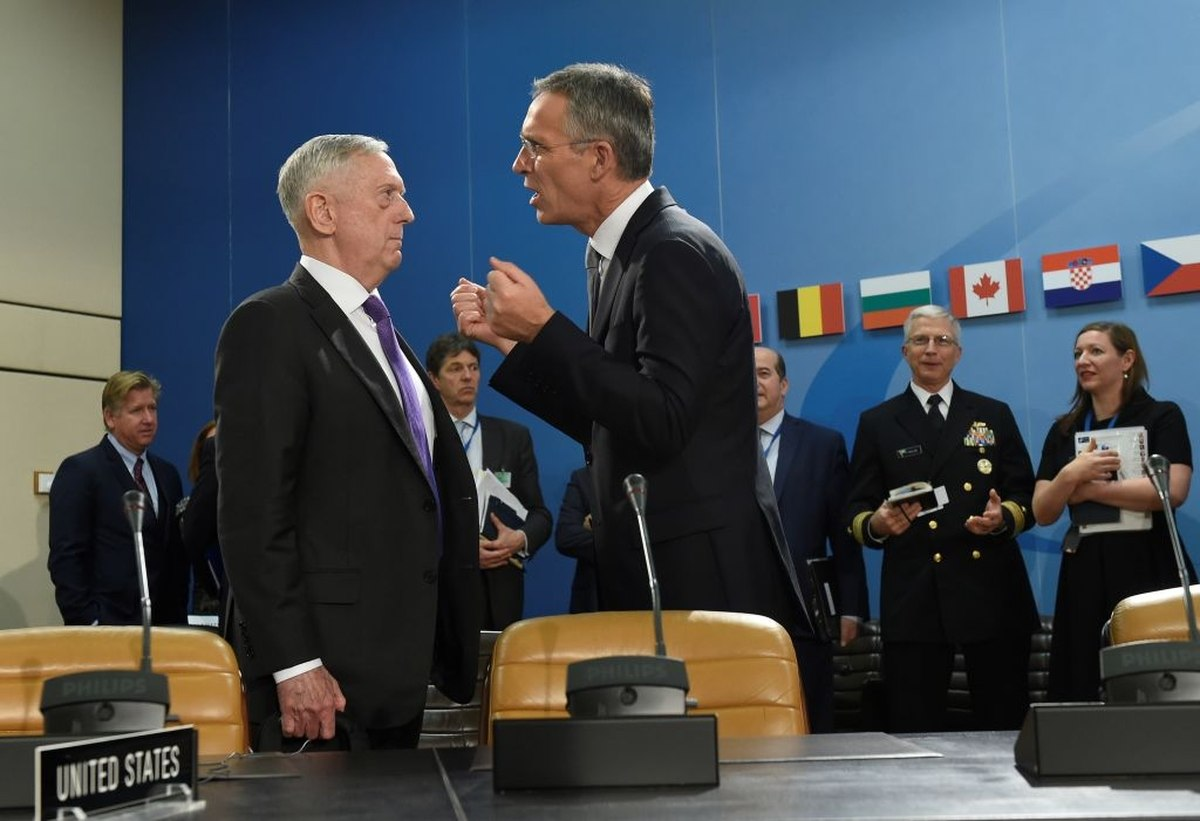
\includegraphics[width=0.95\textwidth]{mattis-nato.jpg}
	\label{fig:mattis-nato}
\end{figure}


\end{frame}

%------------------------------------------------

\begin{frame}[standout]

\huge \textit{Does alliance participation increase military spending?} \uncover<2->{Or decrease it?}

 \end{frame}

%------------------------------------------------

\begin{frame}{Competing Results}

\begin{table}[hbt!]
\begin{center}
\begin{tabular}{lccc}
     & Decrease & Increase & Null \\
\hline
Most \& Siverson 1987  &  &  & X \\
Conybeare 1994 & X & &  \\
Diehl 1994 &  & X &  \\
Goldsmith 2003 &  &  & X \\
Morgan \& Palmer 2006 &  & X & \\ 
Quiroz-Flores 2011 &  & X &  \\ 
Digiuseppe \& Poast 2016 & X &  & \\ 
Horowitz et al 2017 &  & X & \\ 
\hline
\end{tabular}
\end{center} 
\end{table}


 \end{frame}

%------------------------------------------------

\begin{frame}{Omission: Alliance Heterogeneity}


\begin{itemize}
\item Alliances can \textit{increase or decrease} military spending. 
\pause
\item Depends on alliance characteristics. 
\end{itemize} 

\end{frame}

%------------------------------------------------
 \begin{frame}[standout]

Treaty depth is a key sources of differences between alliances. 

 \end{frame}



%------------------------------------------------

\begin{frame}{Outline}

I make my claim about alliance participation and military spending in three ways: 

\pause
\begin{enumerate}
\item Argument: Treaty Depth and Non-Major Powers
\pause
\item Statistical Analysis
\pause
\item Evidence from US alliances
\end{enumerate}


\end{frame}

%------------------------------------------------

\section{Argument}

%------------------------------------------------

\begin{frame}{Assumptions}

\begin{itemize} 
\item States pursue domestic consumption and security. 
\pause 
\item Alliances and military spending both provide security.  
\pause 
\item Military spending has opportunity costs, which decrease with state size. 
\pause 
\item Alliances reduce freedom of action.  
\end{itemize}


\end{frame}

%------------------------------------------------

\begin{frame}{The problem of Free-riding}

Alliances are a form of international cooperation. Free-riding means alliance members:

\begin{enumerate} 
\pause
\item Rely on partners for protection and  
\pause
\item Reduce defense spending.
\end{enumerate}  

\end{frame}

%------------------------------------------------

\begin{frame}{Treaty Depth}

Deep treaties stipulate extensive military support. 

\begin{enumerate} 
\pause
\item The kind of support promised and conditions on support. 
\pause
\item Formal defense cooperation:
\pause
\begin{\itemize}
\item Bases, policy coordination, military aid, side agreements, formal institutions. 
\end{itemize}  
\end{enumerate}  

\end{frame}

%------------------------------------------------

\begin{frame}[standout]

In a deep alliance, free-riding is more difficult.   

\end{frame}


%------------------------------------------------

\begin{frame}{Implications of Treaty Depth}

\begin{enumerate}
\item Alliance members: 
\begin{enumerate} 
\pause
\item Gain more from alliance participation. 
\pause
\item Lose more freedom of action. 
\end{enumerate}  

\end{enumerate}

\end{frame}

%------------------------------------------------

\begin{frame}{Limits on Free-Riding}

There are two ways depth limits alliance members ability to free-ride. 

\begin{enumerate}
\item Greater alliance value.  
\pause
\item Greater allied leverage. 
\end{enumerate}

\end{frame}

%------------------------------------------------

\begin{frame}[standout]

Non-major powers are especially likely to free-ride. 

\end{frame}


%------------------------------------------------

\begin{frame}{Non-Major Powers}

\begin{itemize}
\item Goal: Security.
\pause
\item Constraint: Opportunity Costs of Military Spending.  
\pause
\item Alliance participation usually \emph{decreases} military spending. 
\end{itemize} 

\end{frame}

%------------------------------------------------

\begin{frame}[standout]

\begin{quote}
\textsc{Hypothesis 2}: As alliance treaty depth increases, growth in non-major power military spending from alliance participation will increase. 
\end{quote} 


\end{frame}

%------------------------------------------------

\section{Empirical Analysis} 

%-----------------------------------------------

\begin{frame}{Research Design}

I need two things to test these predictions: 

\pause 
\begin{enumerate} 
\item Measure of treaty depth--- measurement model. 
\pause
\item Connect alliance-level variation with state-level outcomes--- multilevel analysis.  
\end{enumerate} 


\end{frame}

%------------------------------------------------

\begin{frame}{Measuring Treaty Depth}

I use a latent variable model to infer treaty depth from observed promises. 

\pause 

My measure of depth for each alliance is the posterior mean of a latent factor. 

\end{frame} 

%------------------------------------------------

\begin{frame}{Details of Measure}
 
\begin{itemize}
\item Multiple observed indicators of depth (ATOP): 
\begin{itemize} 
\item \textit{Military Support}: offense, defense, neutrality, consultation, non-aggression, unconditional military support.
\item \textit{Other Cooperation}: bases, integrated command, military aid, IO formation, defense policy coordination, other military agreements. 
\end{itemize} 
\pause 
\item Semiparametric mixed factor analysis. (Murray et al 2013)
\pause
\item Generates a posterior distribution of depth for each alliance.
\end{itemize} 


\end{frame} 

%------------------------------------------------

\begin{frame}{Latent Measure of Treaty depth}

% Visual summary of latent measure
\begin{figure}[htbp]
	\centering
		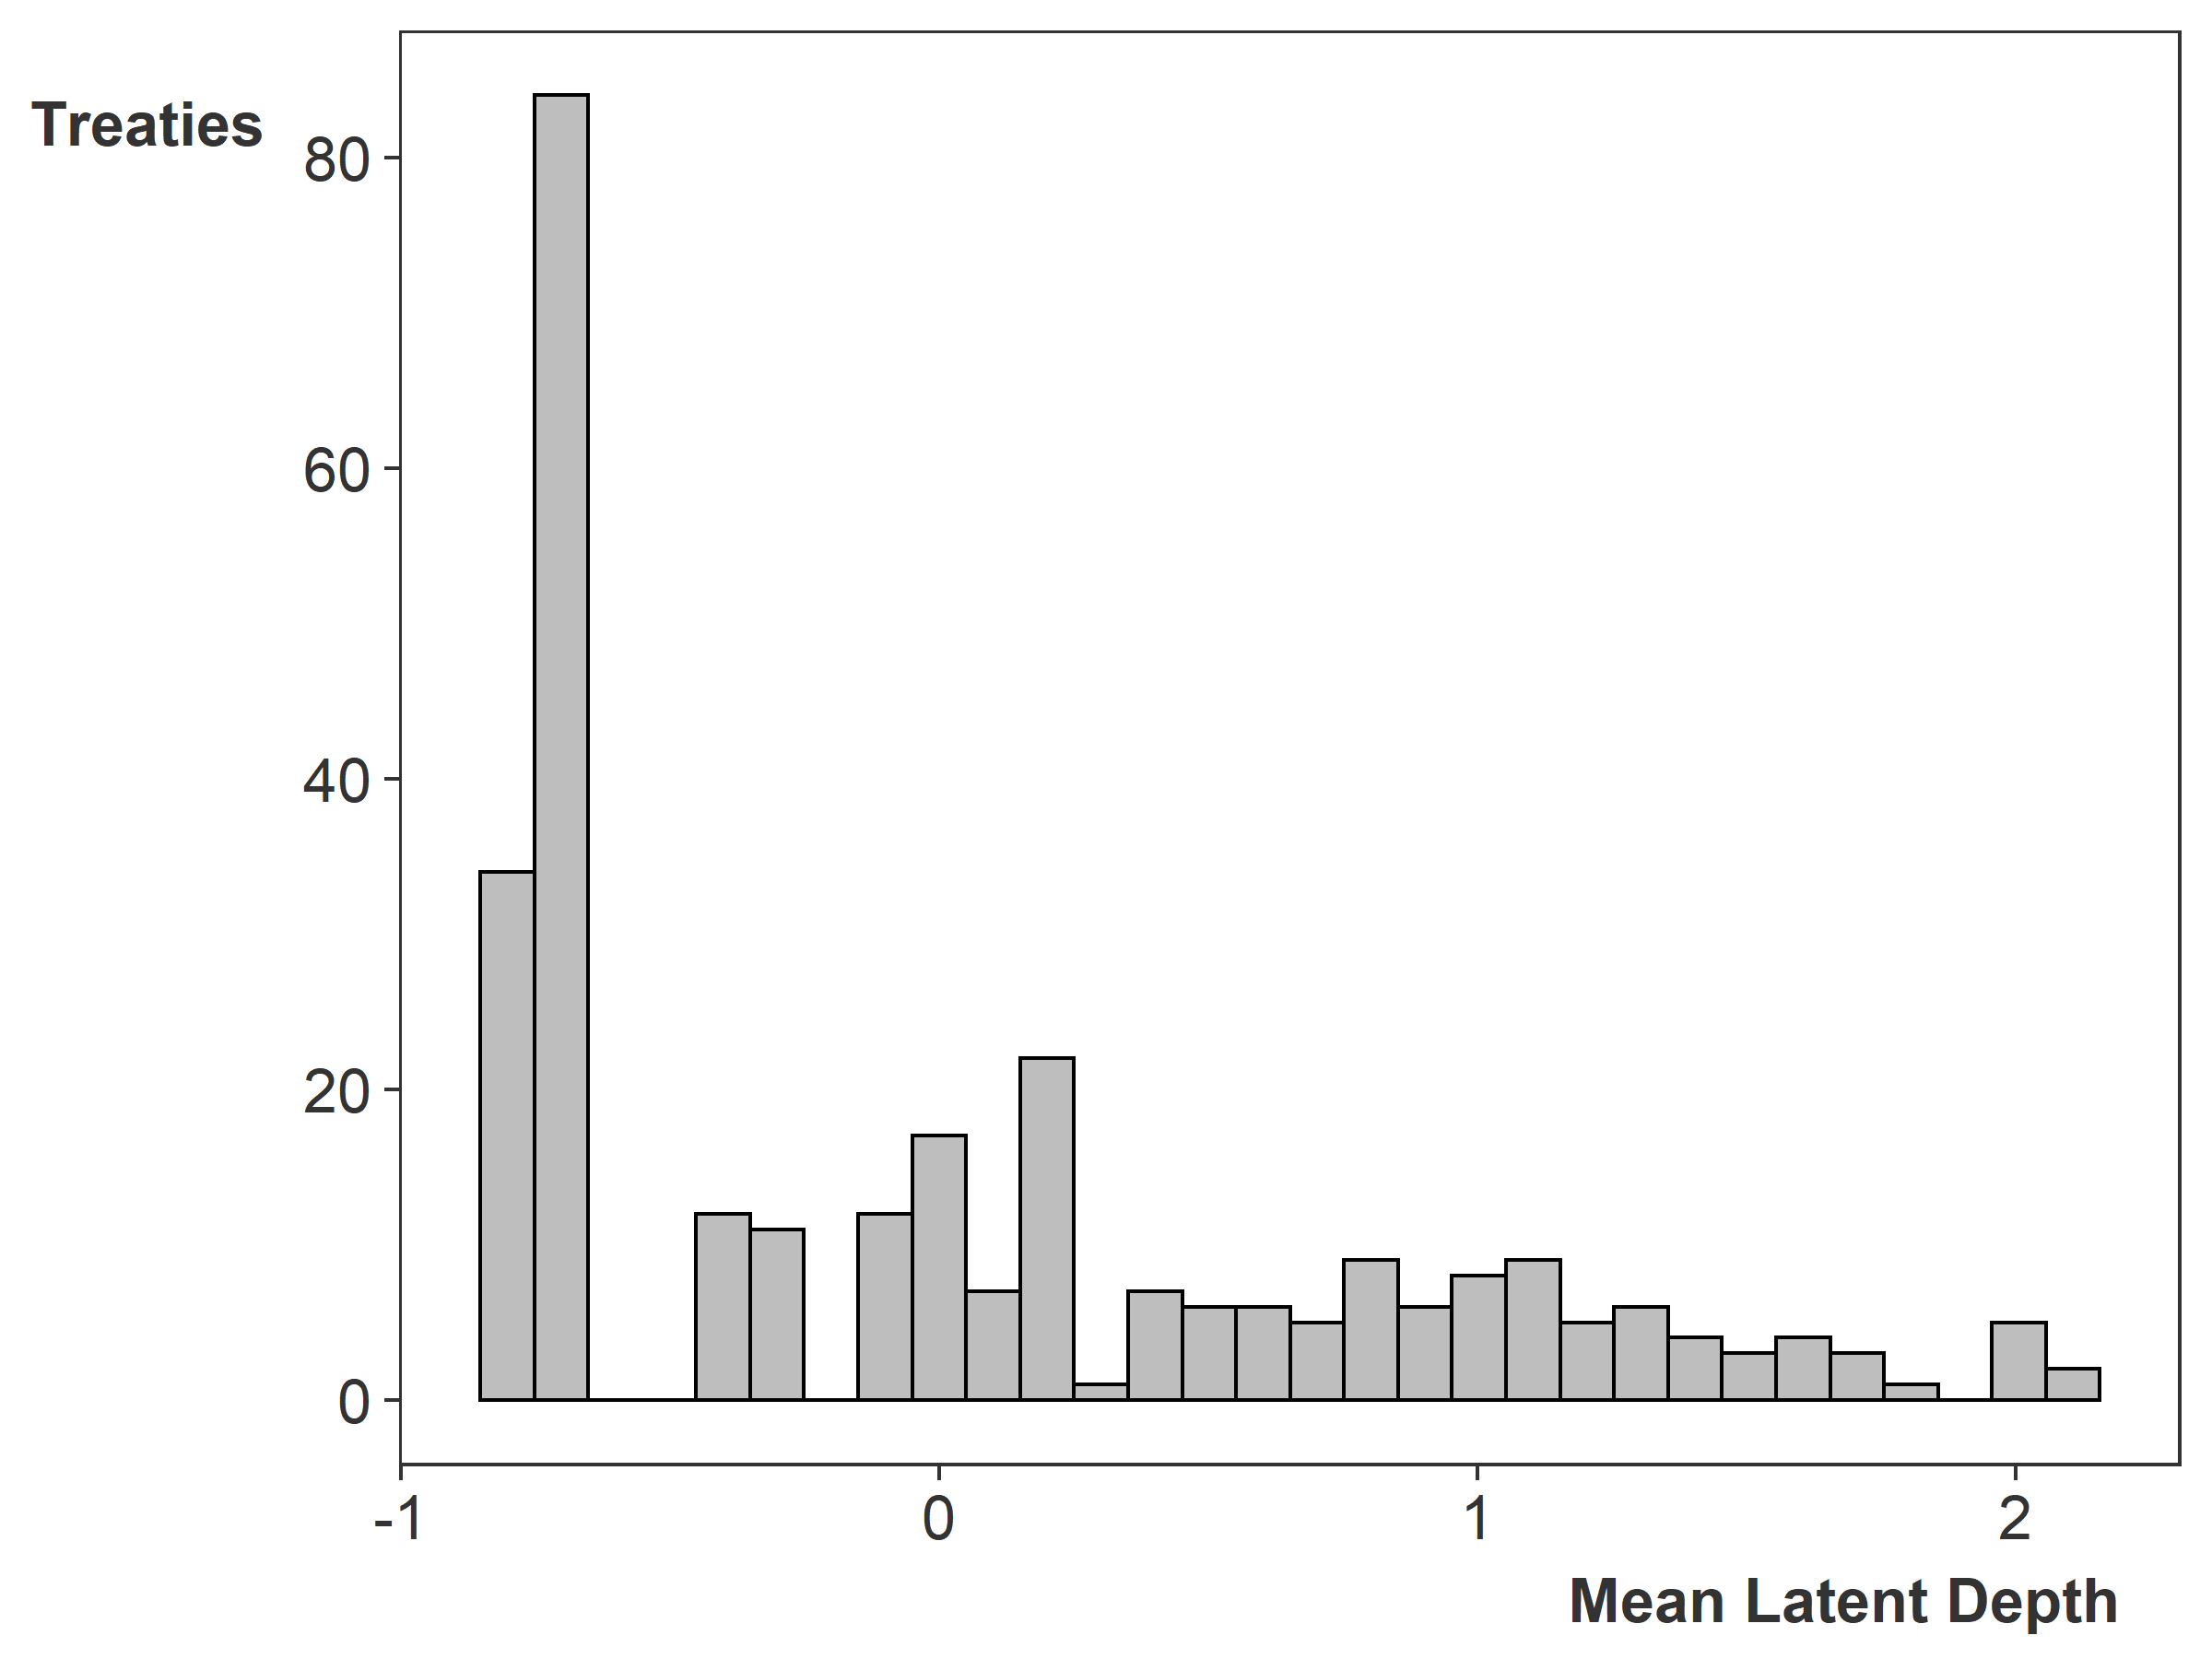
\includegraphics[width=0.95\textwidth]{ld-hist.png}
\end{figure}


\end{frame} 

%------------------------------------------------

\begin{frame}{Latent Measure of Treaty depth: Narrow}

% Visual summary of latent measure
\begin{figure}[htbp]
	\centering
		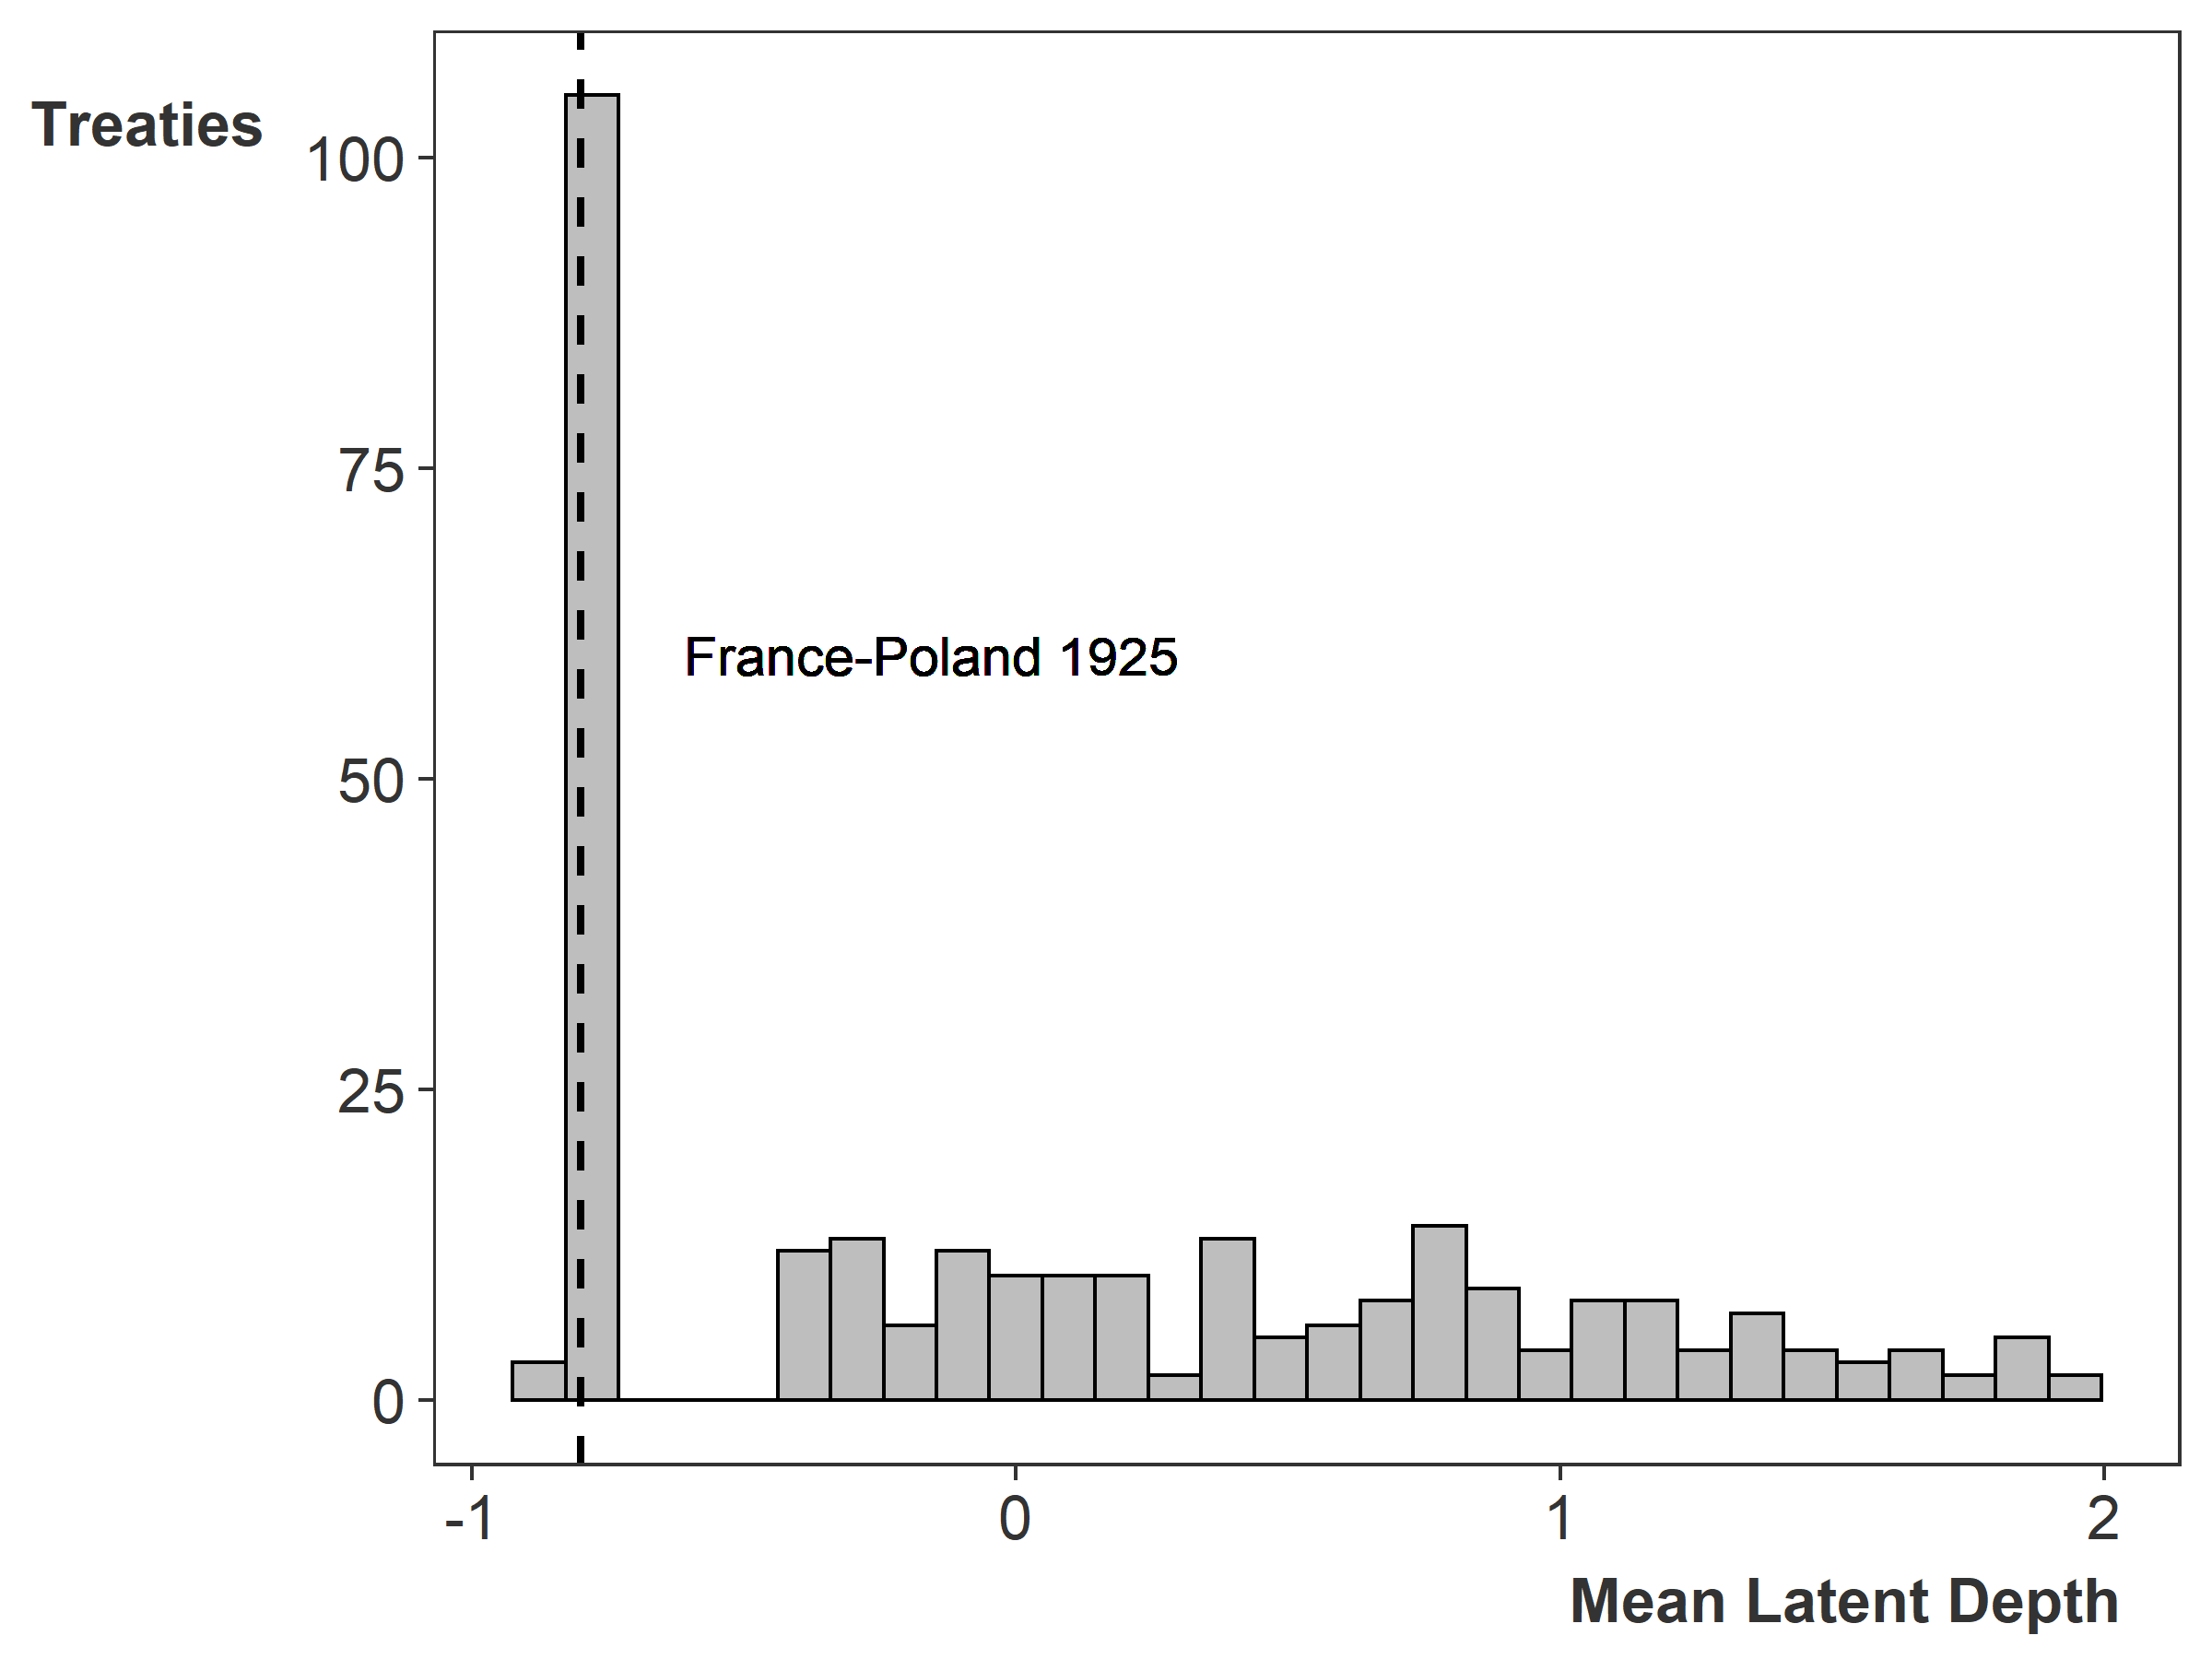
\includegraphics[width=0.95\textwidth]{ld-hist-shallow.png}
\end{figure}


\end{frame} 

%------------------------------------------------

\begin{frame}{Latent Measure of Treaty depth: Typical}

% Visual summary of latent measure
\begin{figure}[htbp]
	\centering
		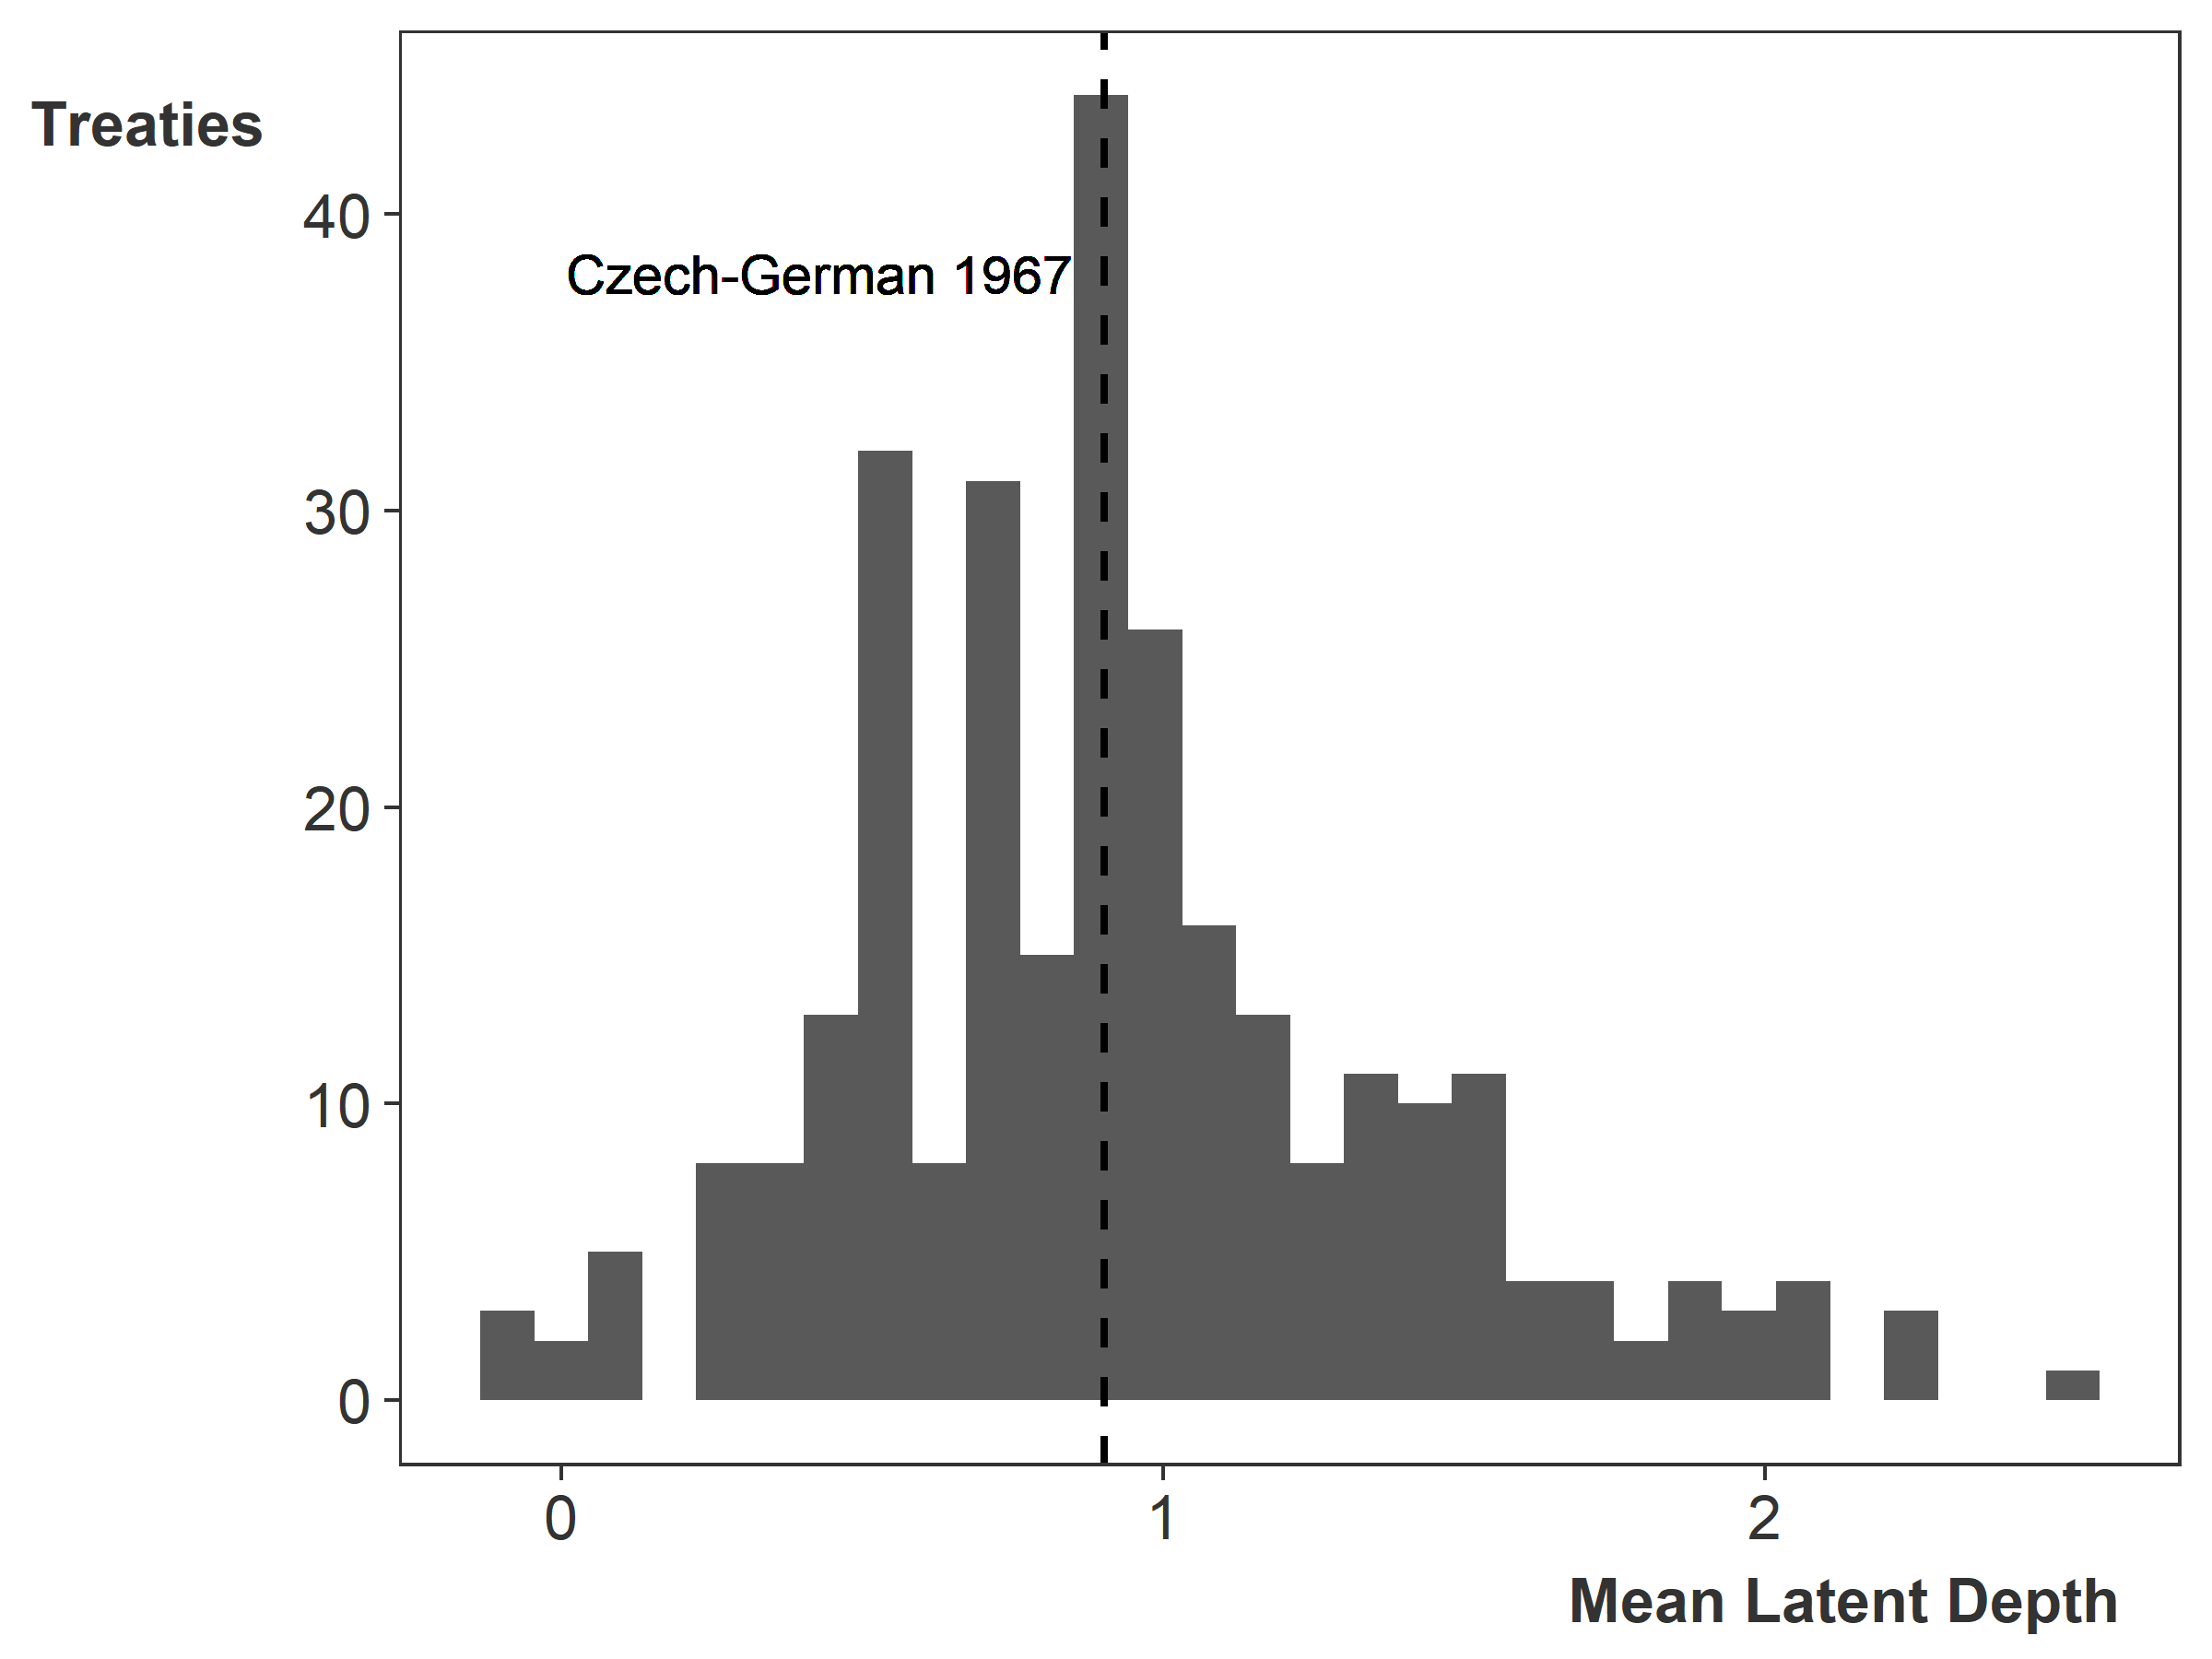
\includegraphics[width=0.95\textwidth]{ld-hist-median.png}
\end{figure}


\end{frame} 

%------------------------------------------------

\begin{frame}{Latent Measure of Treaty depth: Broad}

% Visual summary of latent measure
\begin{figure}[htbp]
	\centering
		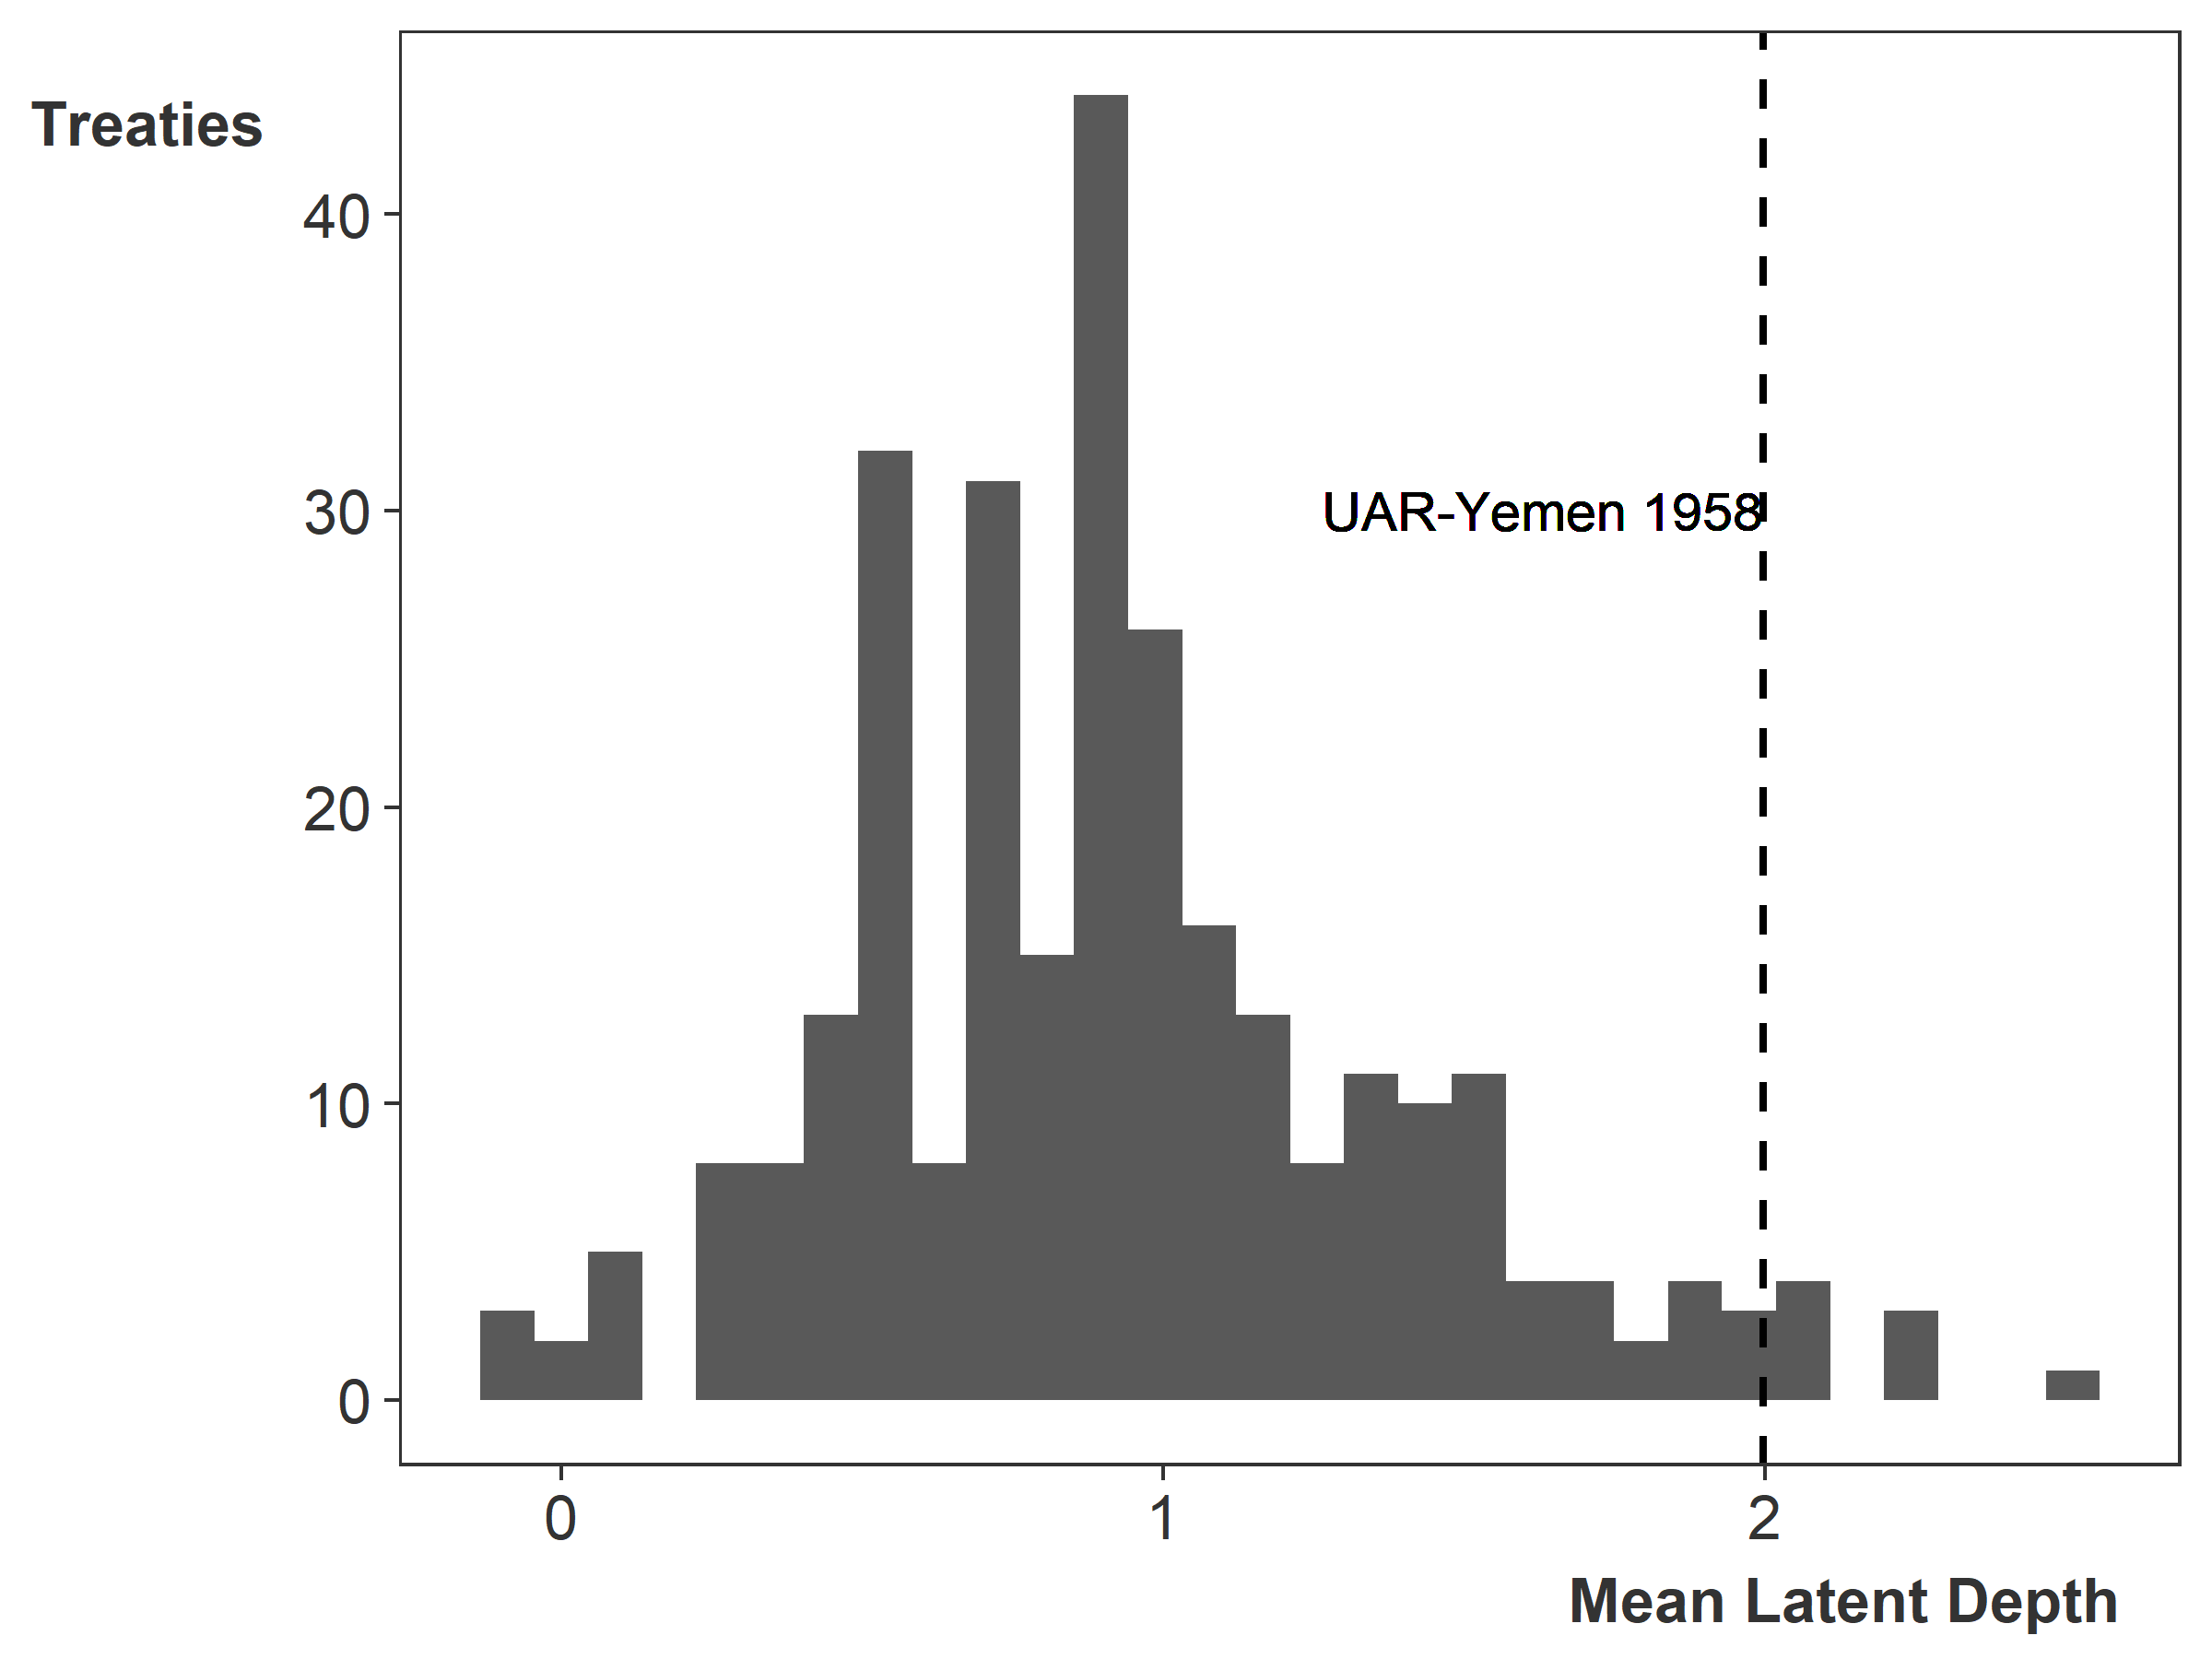
\includegraphics[width=0.95\textwidth]{ld-hist-deep.png}
\end{figure}


\end{frame} 


%------------------------------------------------

\begin{frame}{Empirical Analysis: Multilevel Model}

\begin{itemize} 
\item Link alliance-level variation with state-level outcomes. 
\pause
\item Two connected regressions: alliance and state-level. 
\pause 
\item Alliance characteristics modify the association between alliance membership and spending growth.  
\end{itemize} 

\end{frame} 


%------------------------------------------------

\begin{frame}{ML Model}

\[
\begin{array}{cccccc}
\uncover<2->{ & & & & &\mbox{Alliance} \\
& & & & &    \mbox{Characteristics}  \\
\uncover<3->{& & & & \lambda = & \alpha_{all} + \beta_1 \mbox{depth} + \textbf{X} \beta \\}
& & & & &    \downarrow  \\}
\mbox{Growth} =     & \mbox{Varying}   & + & \mbox{State}   & + & \mbox{Alliance} \\
\mbox{Mil. Ex.}      & \mbox{Intercepts}&   &  \mbox{Vars.} &   & \mbox{Participation} \\
\uncover<3->{\mbox{y} = & \alpha + \alpha^{st} + \alpha^{yr}   & + & \textbf{W} \gamma  & + & \textbf{Z} \lambda \\}
\end{array}
\]


\end{frame}

%------------------------------------------------


\begin{frame}{ML Model Specification}

\begin{equation}
y \sim student_t(\nu, \mu, \sigma)
\end{equation}
\begin{equation}
\mu = \alpha + \alpha^{st} + \alpha^{yr} +\textbf{W}_{n \times k} \gamma + \textbf{Z}_{n \times a} \lambda
\end{equation}

\begin{equation}
\lambda_{a} \sim N(\theta_{a}, \sigma_{all})
\end{equation}
\begin{equation}
\theta_a = \alpha_{all} + \beta_1 \mbox{Treaty depth} + \textbf{X}_{a \times l} \beta
\end{equation}


\end{frame}


%------------------------------------------------

\begin{frame}{Example}

\setbeamercovered{transparent}

\begin{equation*}
\uncover<2->{\mu_{it} =} \uncover<3>{\alpha} \uncover<4>{+ \alpha^{st} + \alpha^{yr}} \uncover<5>{+ W_{it} \gamma} \uncover<6>{+ Z_{it} \lambda}
\end{equation*}

Example year: 

\begin{equation*}
\begin{split}
& \uncover<2->{\mbox{Argentina 1955} = } \uncover<3>{\mbox{Overall mean}} \\
& \uncover<4>{+ \mbox{Argentine Intercept} + \mbox{1955 Intercept}} \\
& \uncover<5>{+ \mbox{Argentine Characteristics}} \\
& \uncover<6>{+ \lambda_{OAS} * \mbox{OAS Expenditure} + \lambda_{Rio} * \mbox{Rio Pact Expenditure}}
\end{split}
\end{equation*}

\uncover<7>{
\begin{equation*}
\lambda_{Rio} = \alpha_{all} + \beta_1 0.717 + \mbox{Controls}
\end{equation*}
} 


\end{frame}


%------------------------------------------------


\begin{frame}[standout]{Z} 

\begin{tabular}{lccc}
State-Year & Rio Pact & Warsaw Pact & \ldots \\
\hline
Argentina 1954 & .347 & 0 & \ldots \\
Argentina 1955 & .418  & 0 & \ldots  \\
 \vdots & \vdots & \vdots & \ldots  
\end{tabular}

 \end{frame}



%------------------------------------------------

\begin{frame}{Sample and Key Variables}

\begin{itemize}
\item \textbf{Split Sample}: major and non-major power states--- 1816-2007. Alliances with military support. 
\pause
\item \textbf{DV}: Growth in Military Spending $ = \frac{ \Delta \mbox{Mil. Expend}_t }{ \mbox{Mil. Expend}_{t-1} }$ 
\pause
\item \textbf{Alliance-Level IV}: Mean Treaty depth
\end{itemize} 

\end{frame}


%------------------------------------------------

\begin{frame}{Controls}

\begin{itemize}
\item \textbf{State-Level Controls}: Interstate war, Civil War, Annual MIDs, GDP growth, POLITY, Cold War, Rival military expenditures. 
\pause 
\item \textbf{Alliance-Level Controls}: Share of Democracies, Number of Members, wartime, asymmetric obligations, US member (Cold War), USSR member.

\end{itemize} 

\end{frame}


%------------------------------------------------

\subsection{Results}

%------------------------------------------------

\begin{frame}{Association Between Treaty depth and Growth in Military Spending} 

\begin{figure}
	\centering
		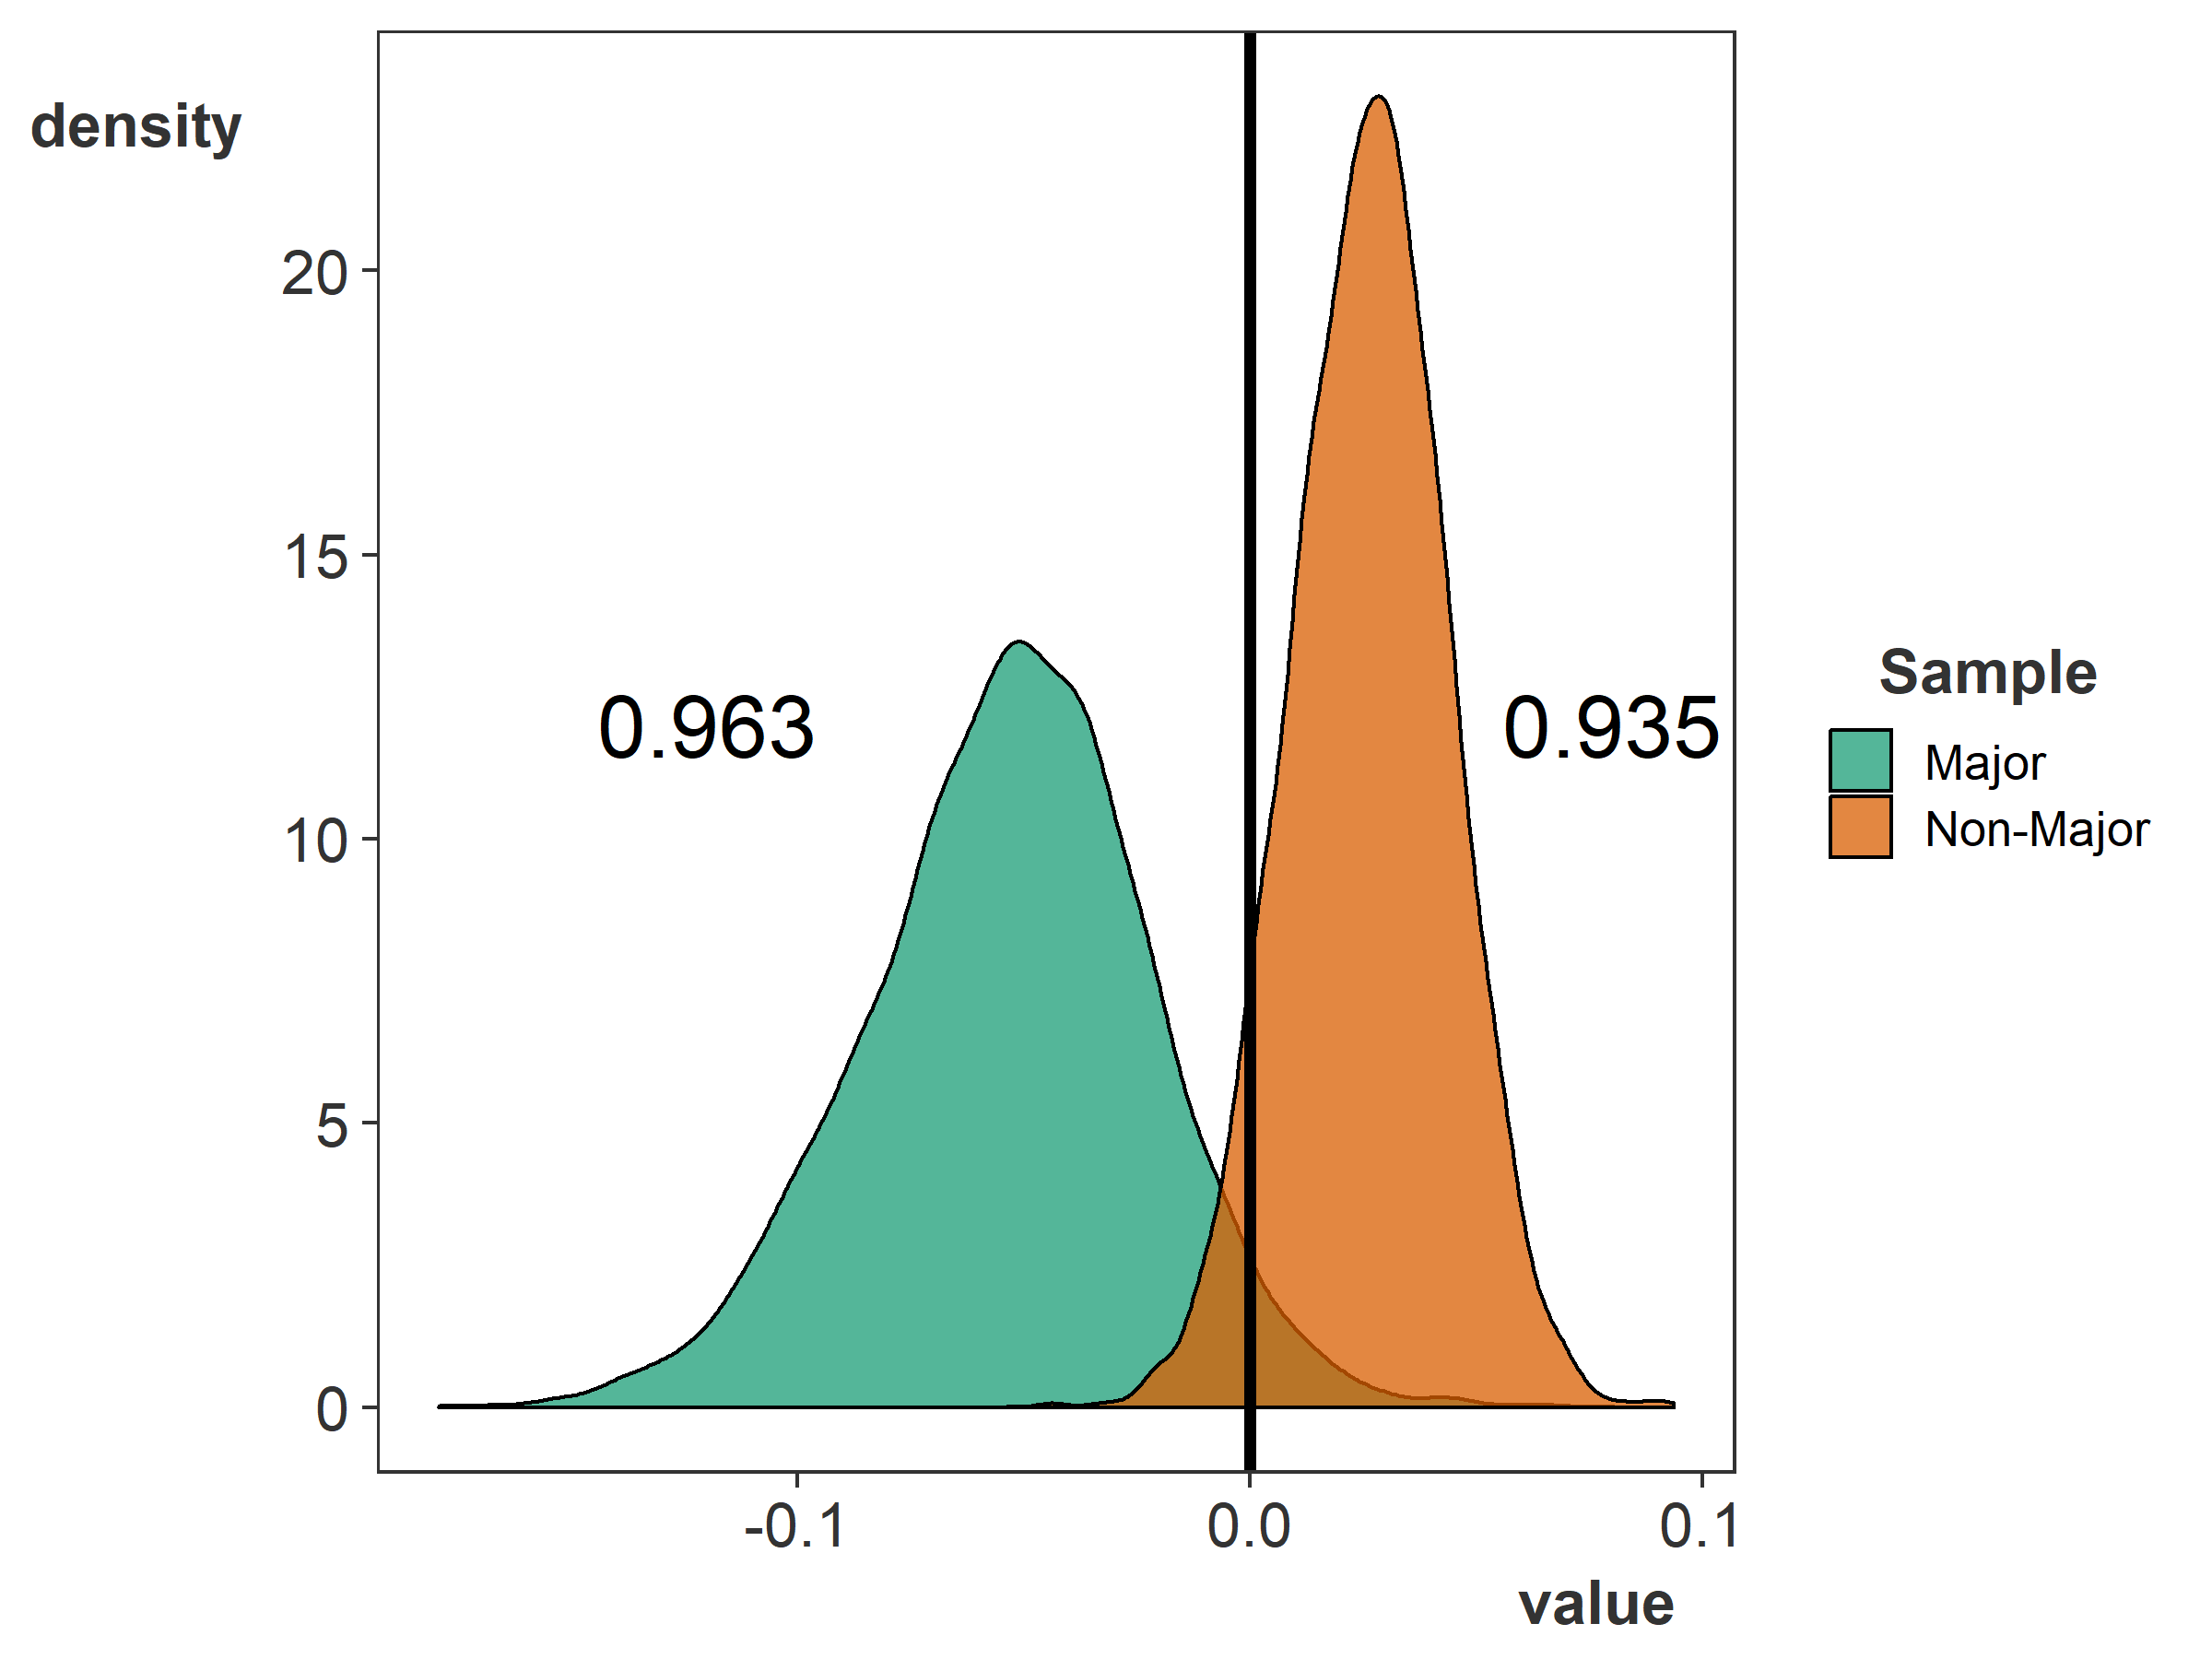
\includegraphics[width=0.95\textwidth]{str-post.png}
	\label{fig:str-post}
\end{figure}


\end{frame}


%------------------------------------------------

\begin{frame}[standout]{Importance} 

\begin{tabular}{lcc}
Sample & Post. Mean & Median Growth \\
\hline
Major & -0.05 & 0.04 \\
\pause
Non-major & 0.03 & 0.06  \\
\end{tabular}

\pause

US spent \$36.0 billion on NATO in 2018, or 5.5\% of the total defense spending. 


\end{frame}

%------------------------------------------------


\begin{frame}{Treaty depth and $\lambda$}

\begin{figure}[htbp]
	\centering
		\includegraphics[width=0.95\textwidth]{ls-lambda-blank.png}
	\label{fig:ls-lambda-blank}
\end{figure}


\end{frame}

%------------------------------------------------


\begin{frame}{Treaty depth and $\lambda$: Major Powers}

\begin{figure}[htbp]
	\centering
		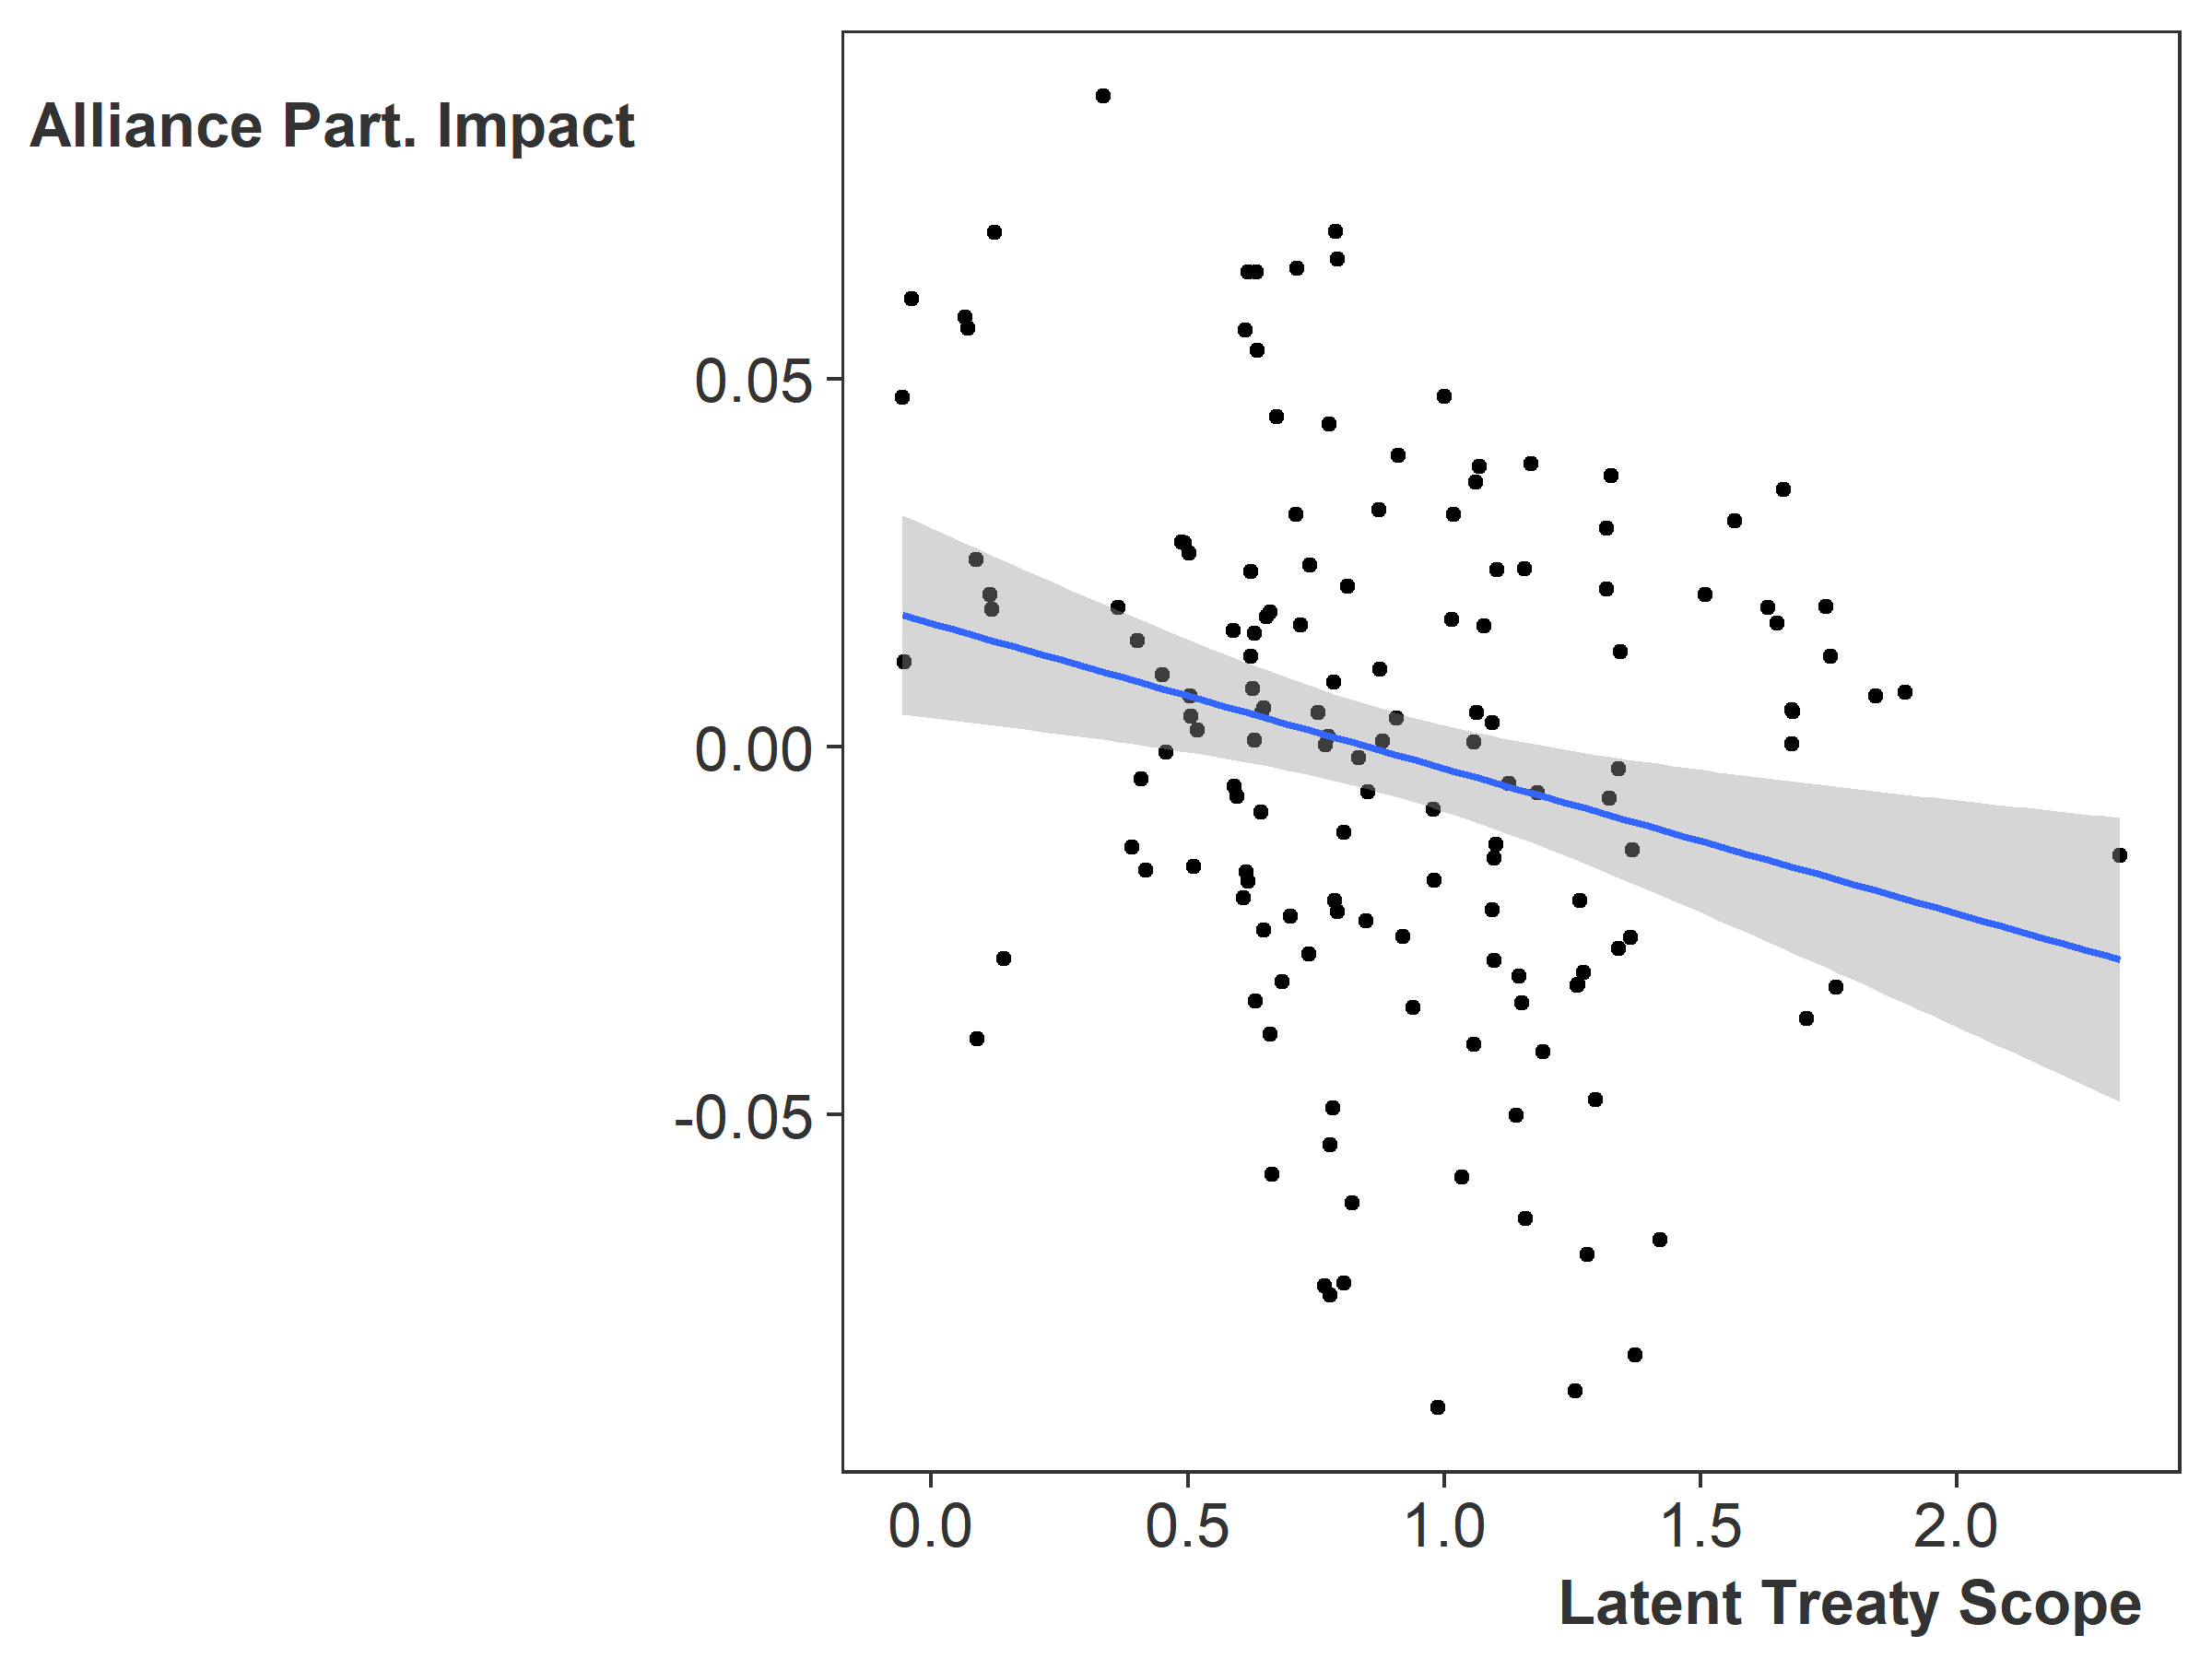
\includegraphics[width=0.95\textwidth]{ls-lambda-maj.png}
	\label{fig:ls-lambda-maj}
\end{figure}


\end{frame}


%------------------------------------------------

\begin{frame}{Treaty depth and $\lambda$: Non-major Powers}

\begin{figure}
	\centering
		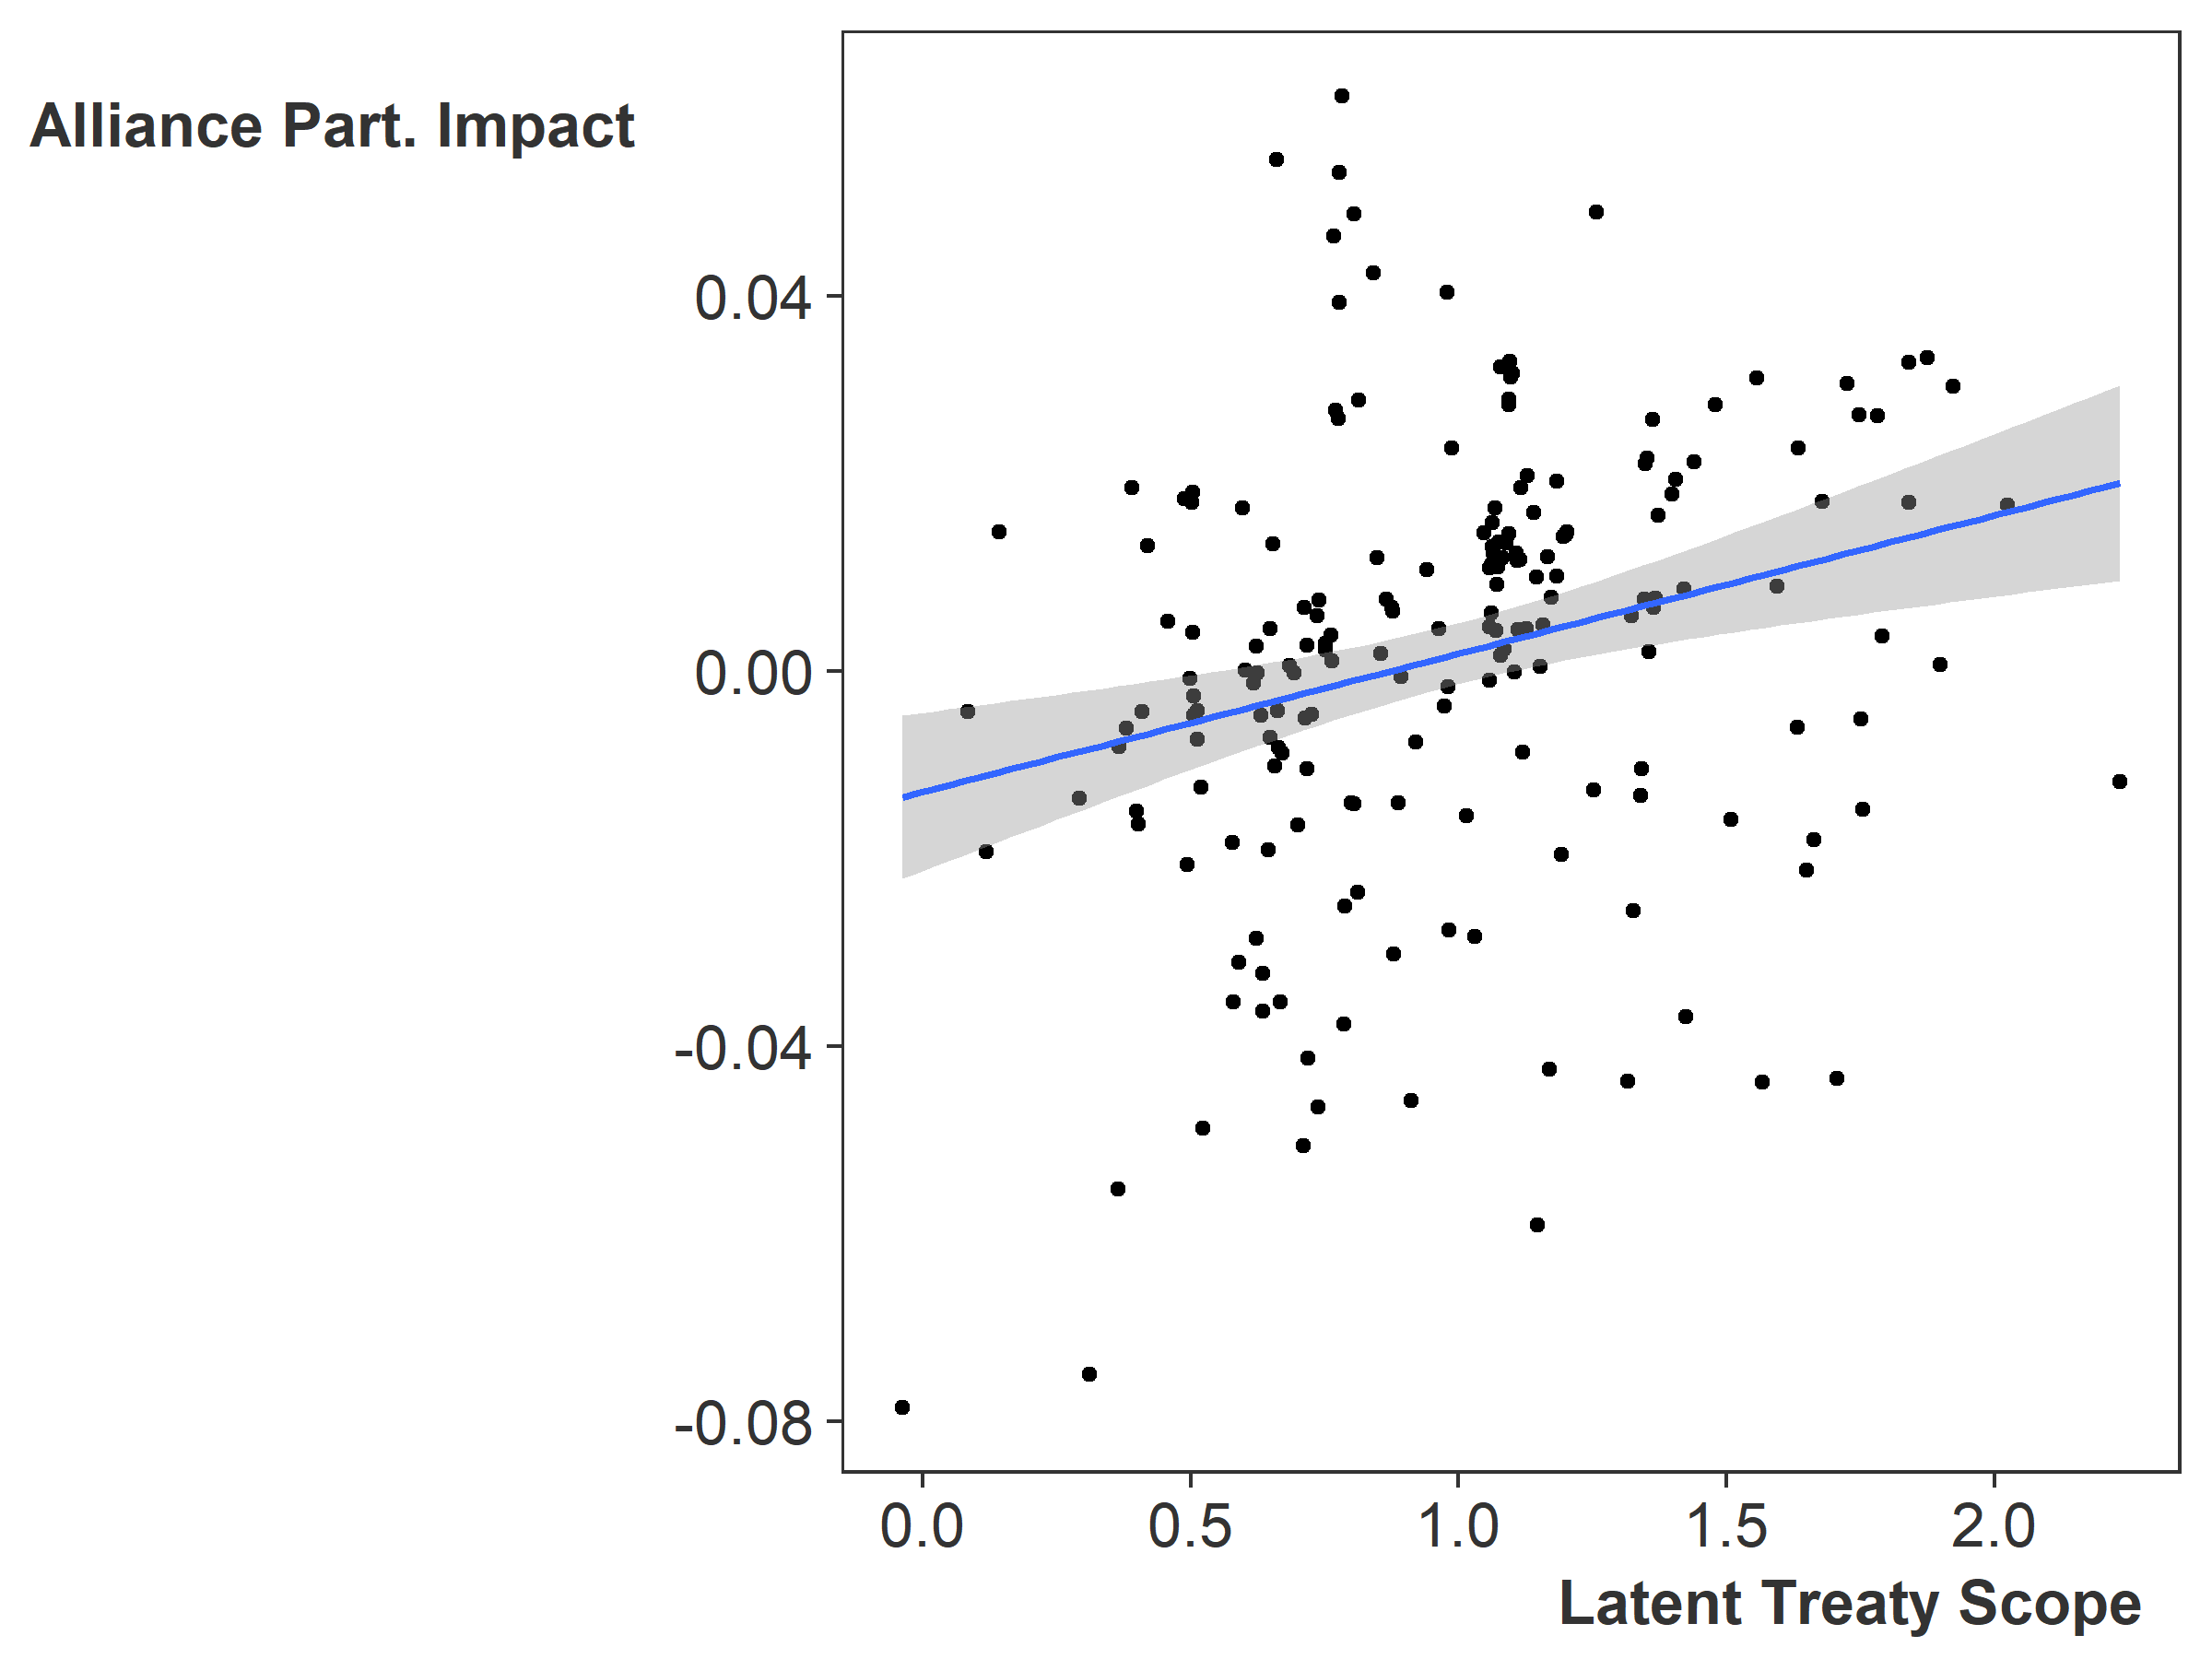
\includegraphics[width=0.95\textwidth]{ls-lambda-min.png}
	\label{fig:ls-lambda-min}
\end{figure}


\end{frame}

%------------------------------------------------

\section{US Alliances}

%------------------------------------------------

\begin{frame}{Foreign Entanglement and Formal Obligations}

\begin{figure}
	\centering
		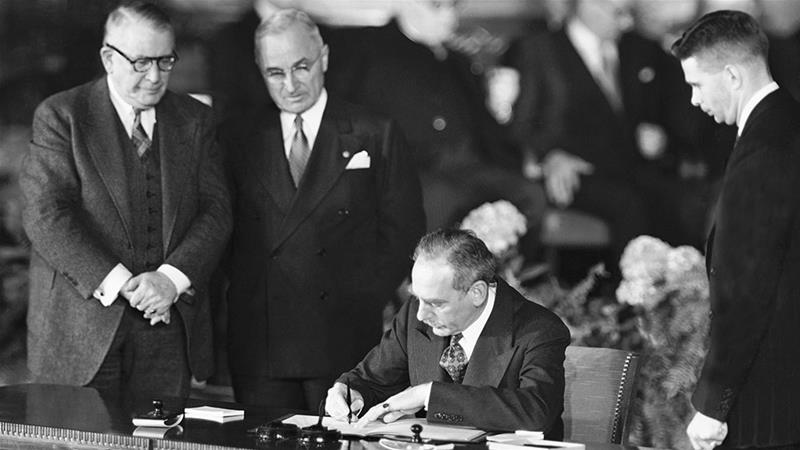
\includegraphics[width=0.95\textwidth]{acheson-nato-sign.jpg}
	\label{fig:acheson-nato-sign}
\end{figure}


\end{frame}

%------------------------------------------------

\begin{frame}[standout]

\large ``The Parties agree that an armed attack against one or more of them in Europe or North America shall be considered an attack against them all...'' 

 \end{frame}

%------------------------------------------------

\begin{frame}[standout]

\large ``assist the Party or Parties so attacked by taking forthwith, individually and in concert with the other Parties, such action as it deems necessary, including the use of armed force'' 

 \end{frame}

%------------------------------------------------

\begin{frame}[standout]

\huge ``such action as it deems necessary, including the use of armed force'' 

 \end{frame}

%------------------------------------------------

\begin{frame}{NATO depth} 

\begin{figure}
	\centering
		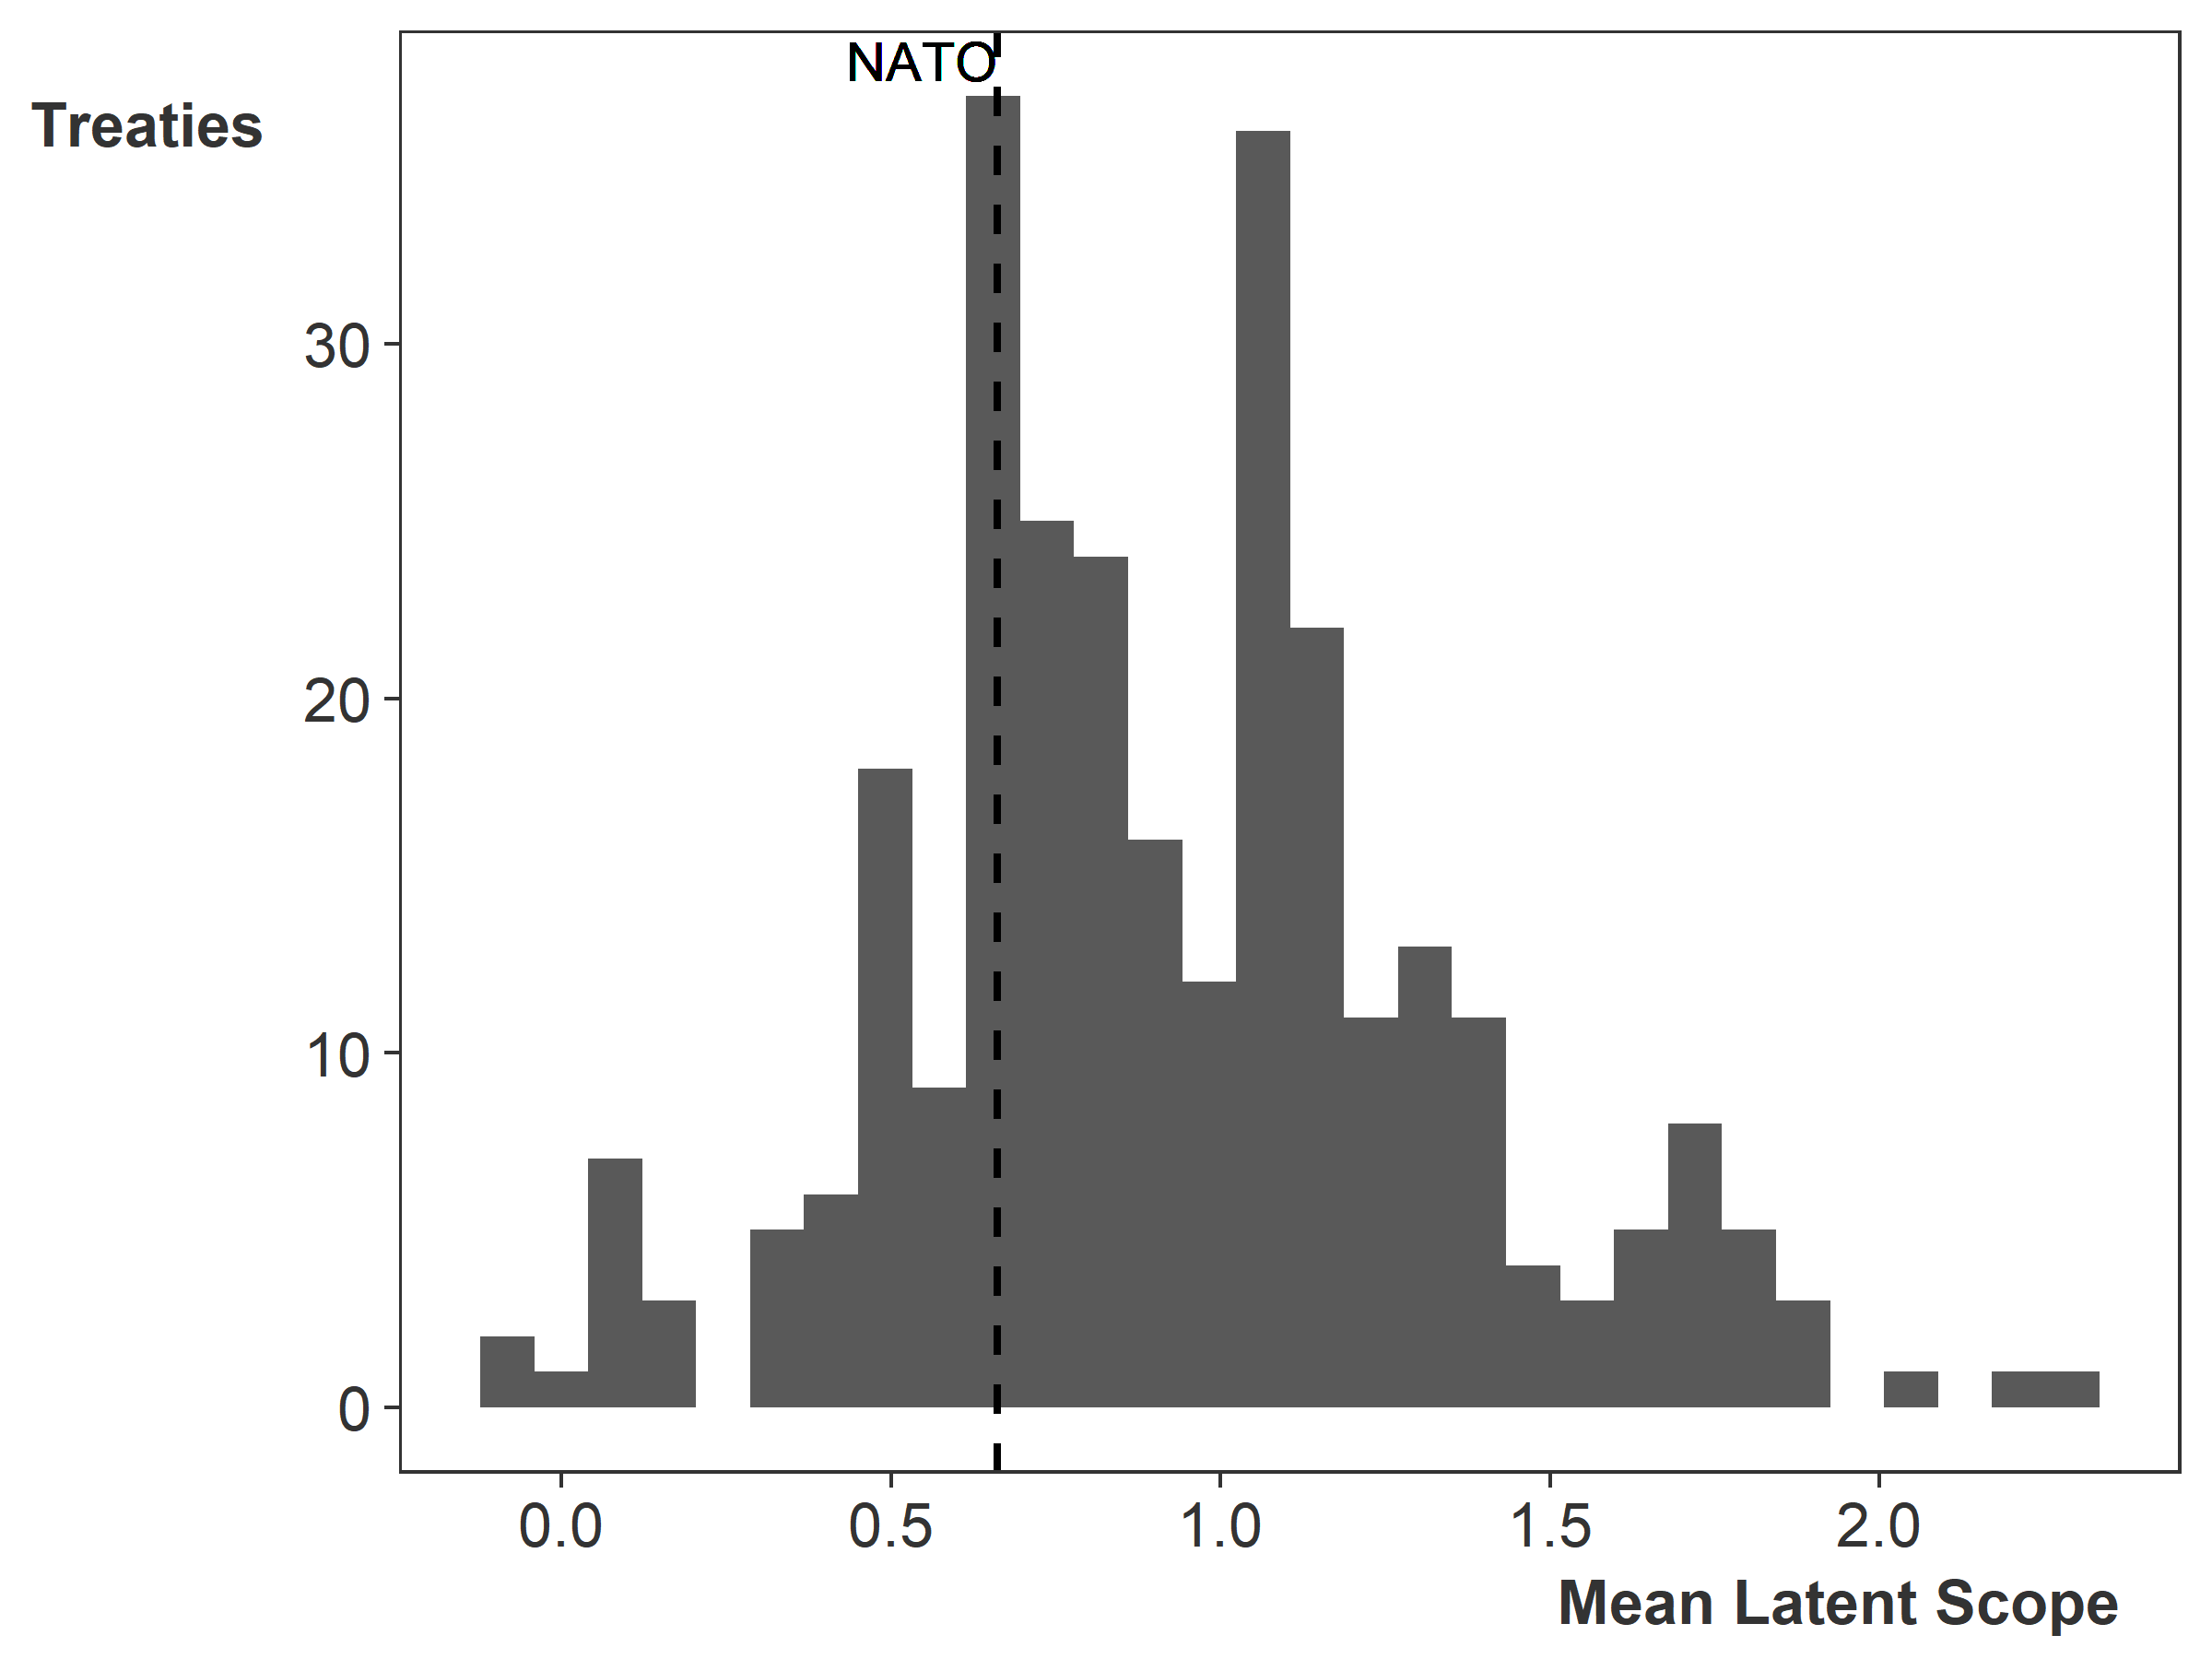
\includegraphics[width=0.95\textwidth]{ls-hist-nato.png}
\end{figure}


 \end{frame}

%------------------------------------------------

\begin{frame}{Impact of NATO on Growth in US Military Spending} 

\begin{figure}
	\centering
		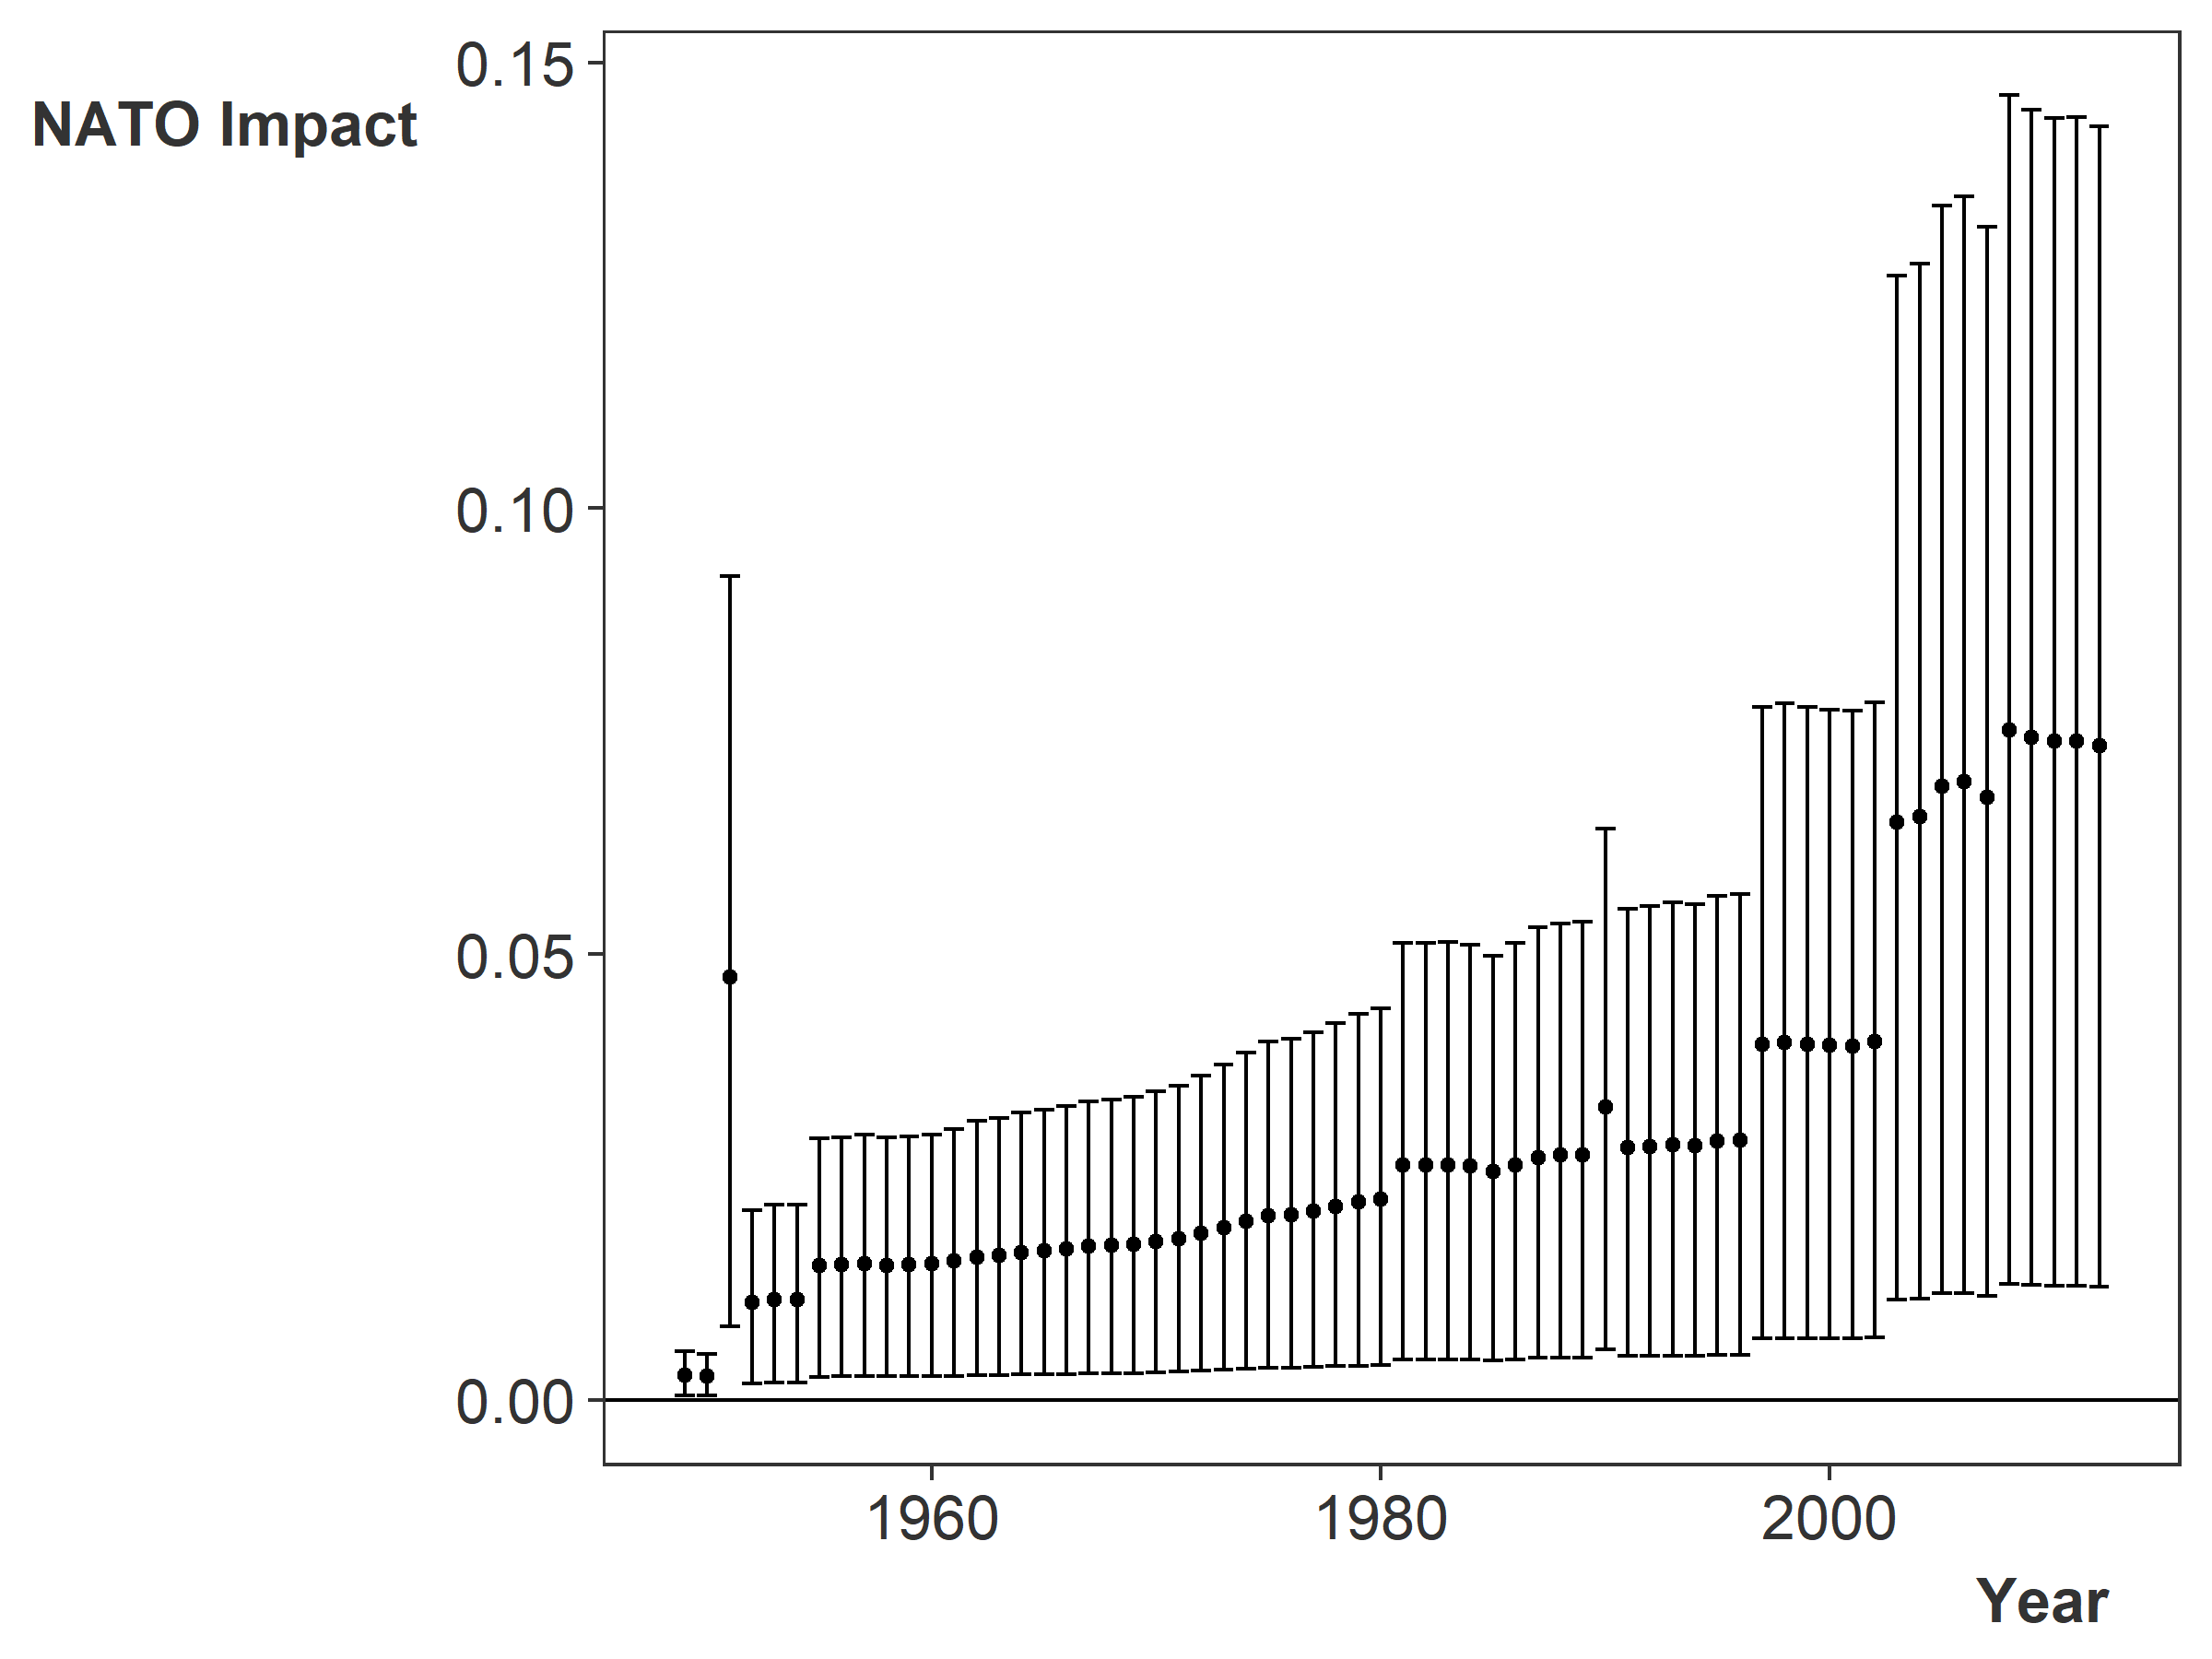
\includegraphics[width=0.95\textwidth]{nato-imp-us.png}
\end{figure}

\end{frame}



%-----------------------------------------------

\begin{frame}{Implication: What to do with US alliances?}

\begin{figure}[htbp]
	\centering
		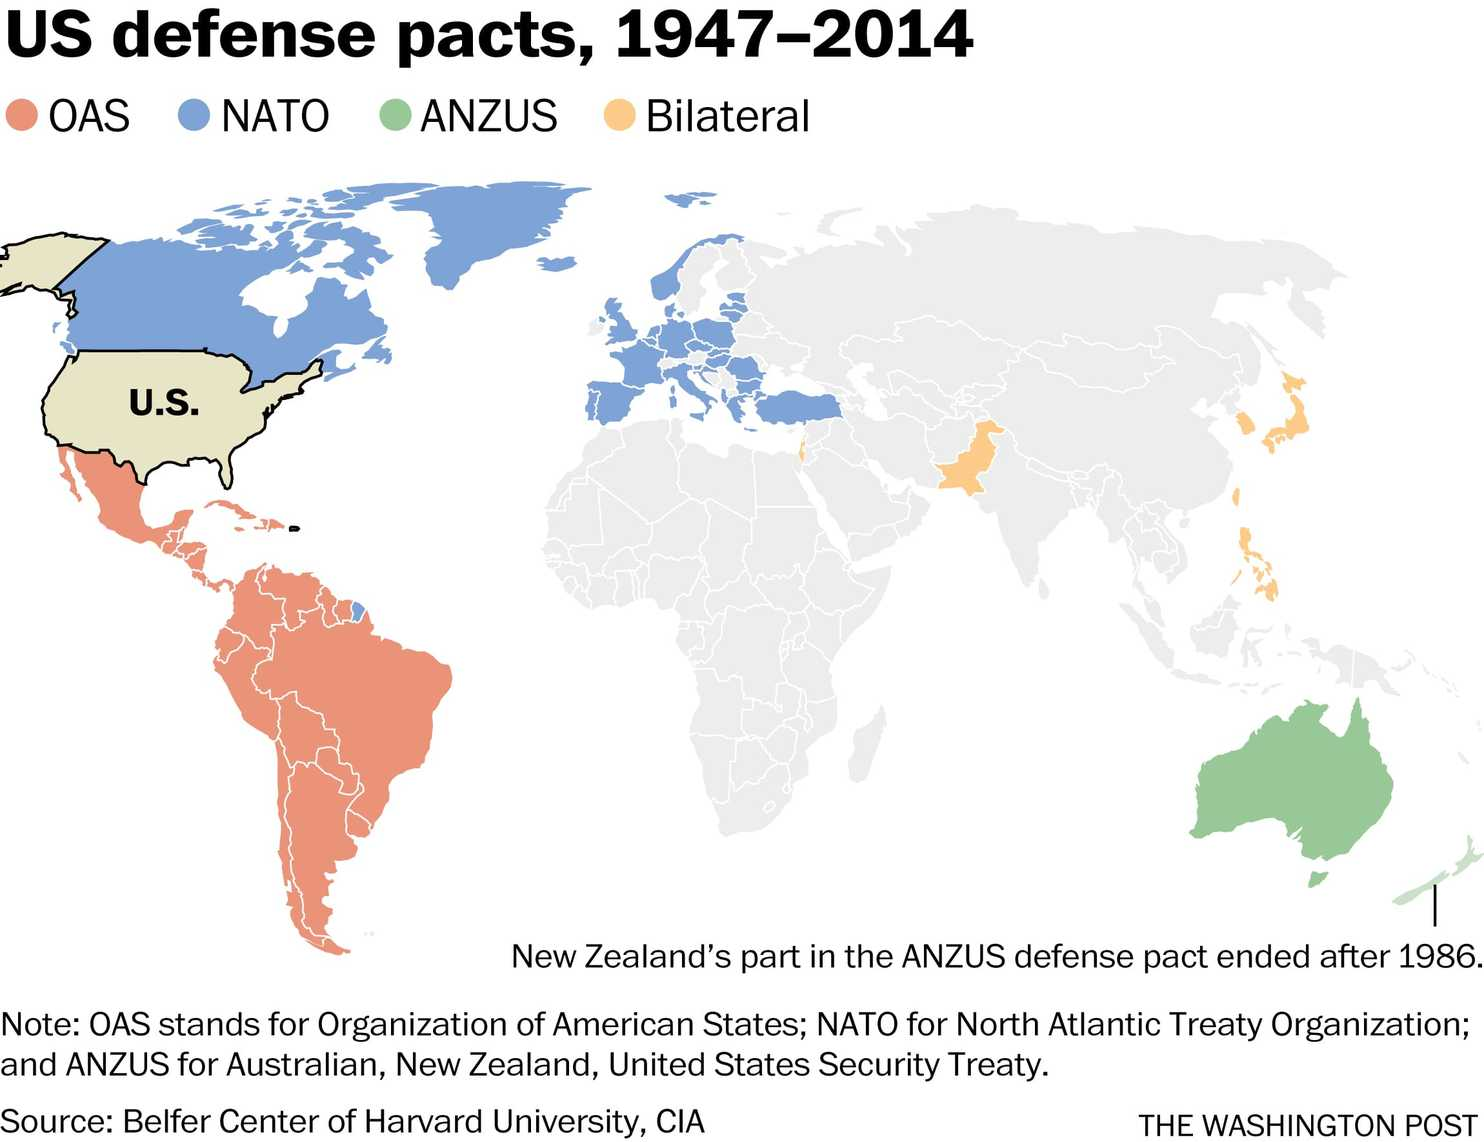
\includegraphics[width=0.95\textwidth]{nato-map.jpg}
\end{figure}


\end{frame}


%-----------------------------------------------

\begin{frame}{Alliance Participation and US Military Spending}

\begin{figure}[htbp]
	\centering
		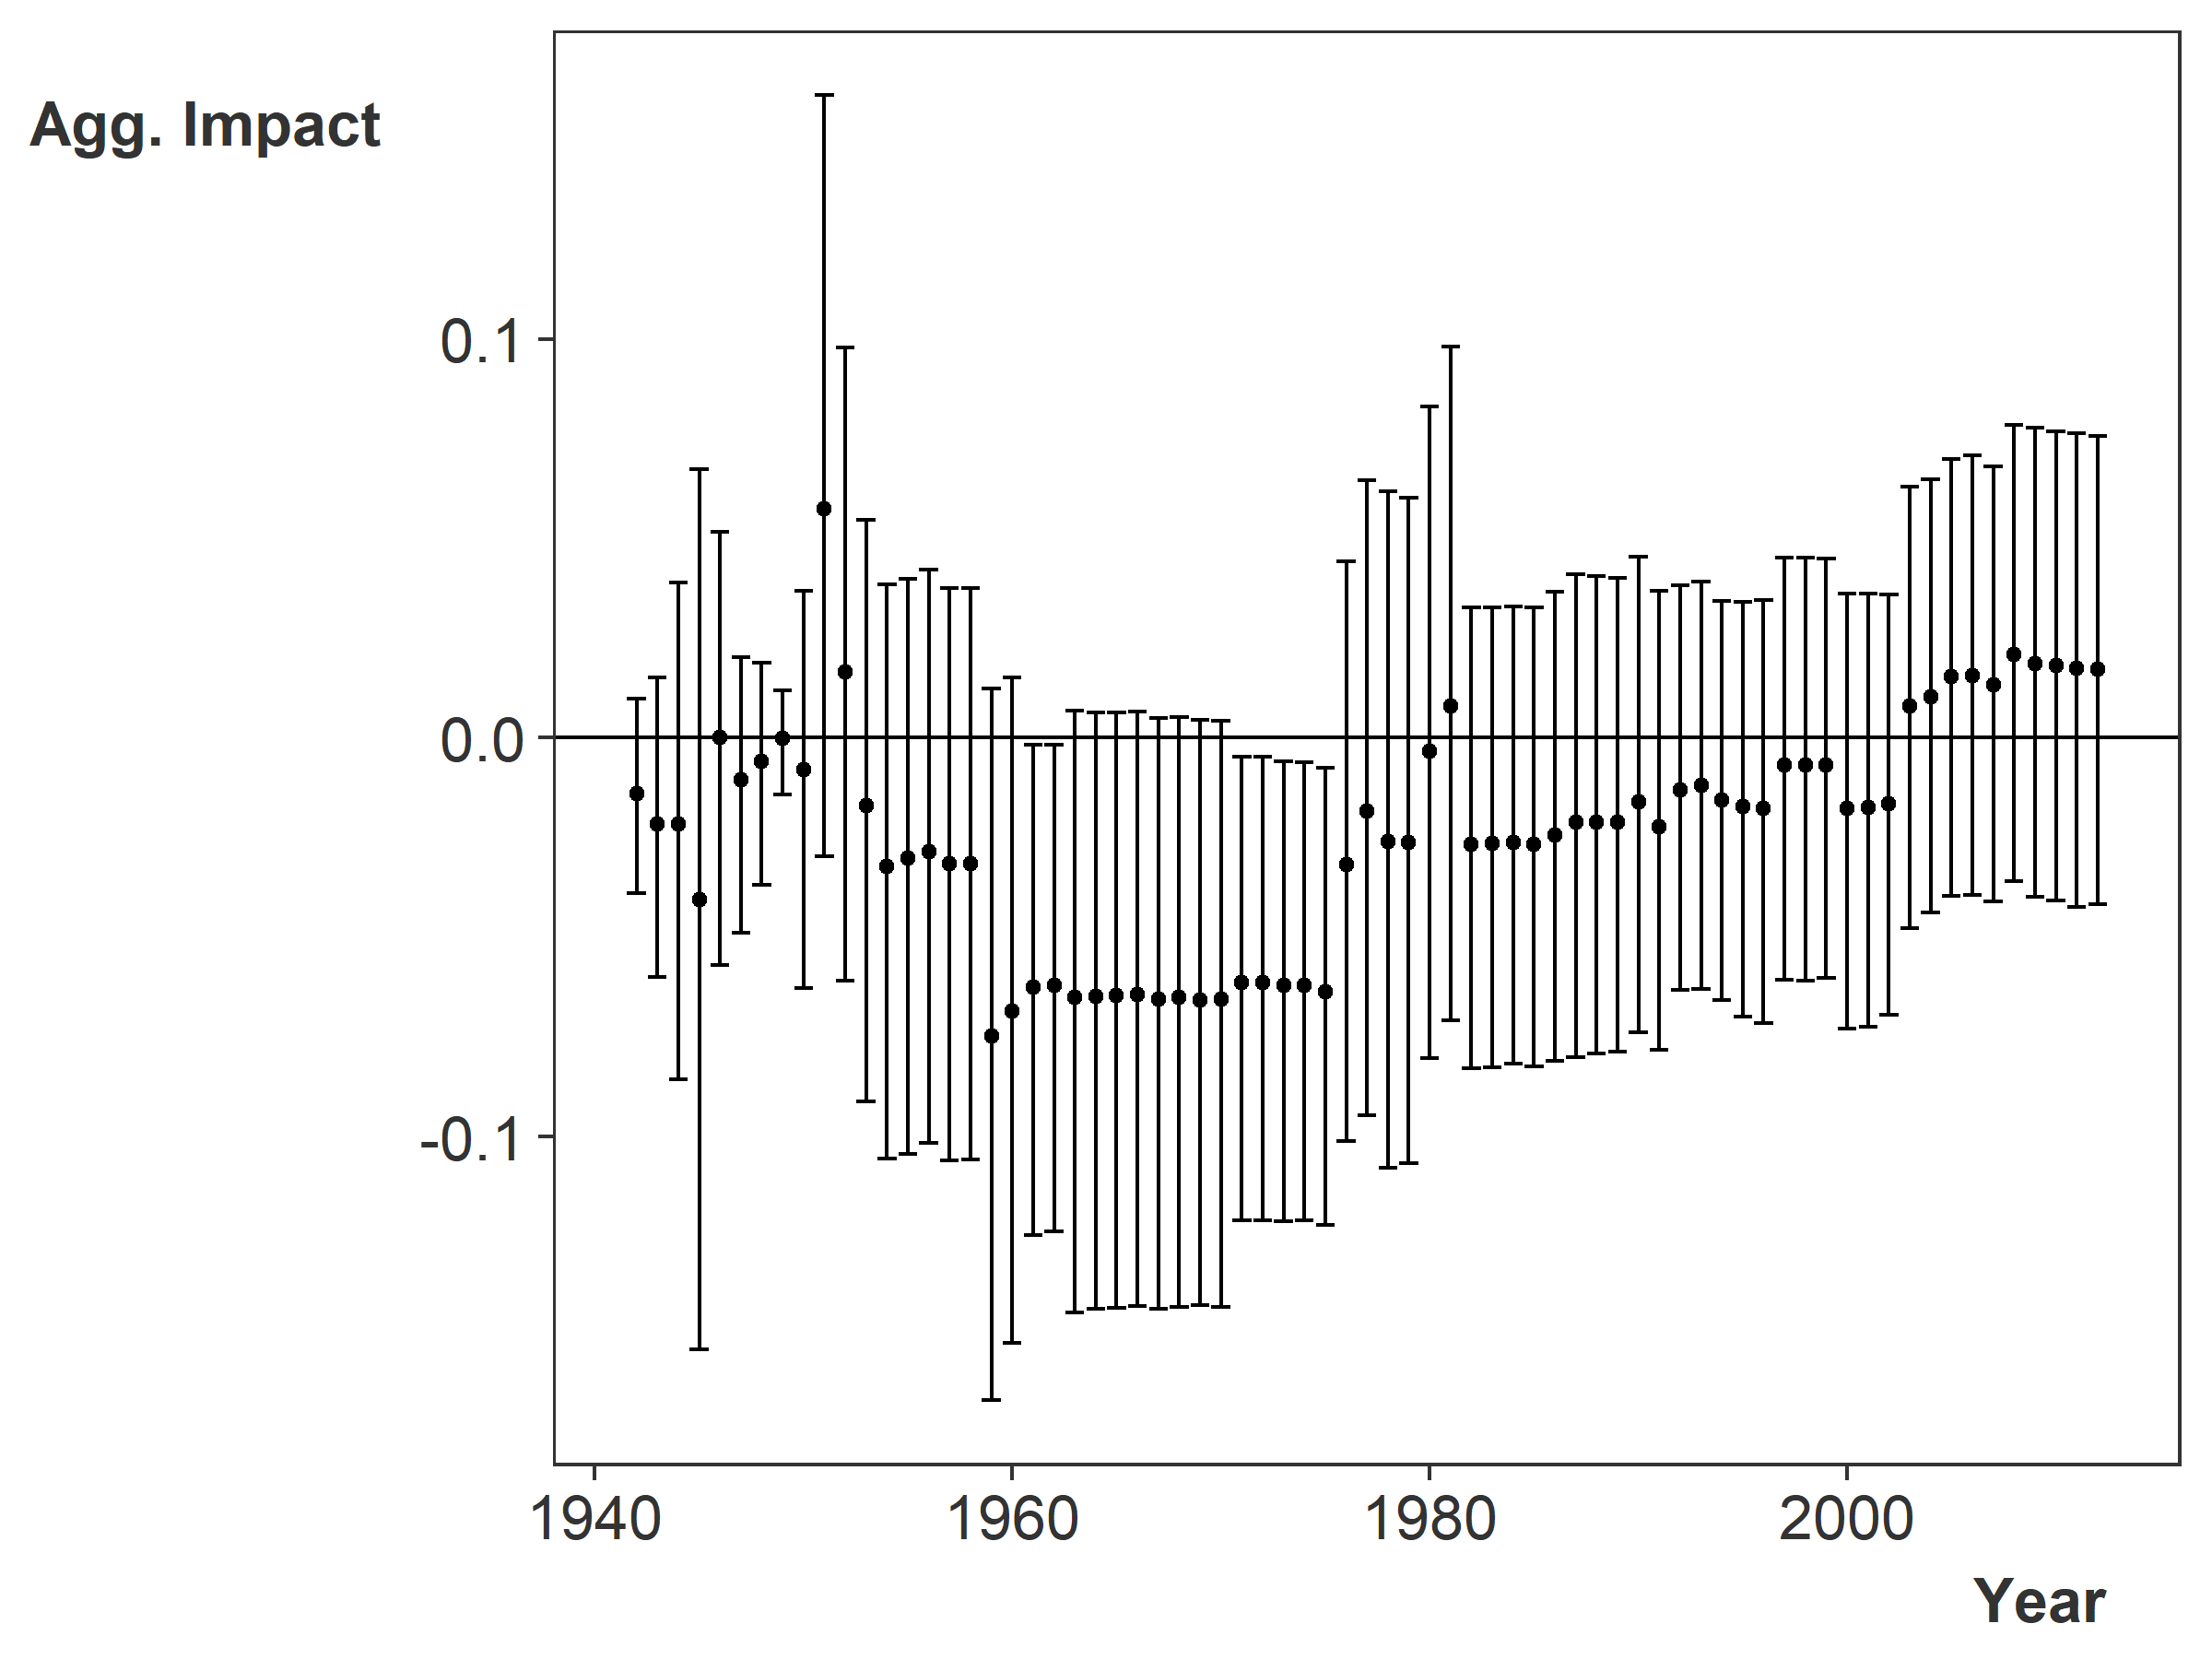
\includegraphics[width=0.95\textwidth]{us-agg-imp.png}
\end{figure}

\end{frame}


%-----------------------------------------------

\section{Conclusion}

%-----------------------------------------------

\begin{frame}[standout]

How alliance participation affects military spending depends on state capability and treaty depth.  

\end{frame}

%------------------------------------------------
% The two subpoints 
 \begin{frame}[standout]

\setbeamercovered{invisible}

\uncover<1-2>{1: Though alliance participation usually increases major power military spending, growth is lower in broad treaties.} 

\uncover<2>{2: Though alliance participation usually decreases non-major power military spending, growth is higher in broad treaties.}

 \end{frame}


%-----------------------------------------------

\section{Looking Ahead}

%-----------------------------------------------

\begin{frame}{Dissertation}

My dissertation articulates and tests a more general theory of alliance participation and military spending. 

\end{frame}


%-----------------------------------------------


\begin{frame}{My Research Agenda}

The political economy of security, with a focus on formal institutions. 

\begin{columns}

% Major powers
\begin{column}{0.5\textwidth}
\textbf{International Security}
\begin{itemize} 
\item Alliance Participation and Military Spending 
\item Reassessing the Public Goods Theory of Alliances
\end{itemize} 
\end{column}



\begin{column}{0.5\textwidth}
\textbf{Intra-State Conflict}
\begin{itemize}
\item Conflict Management Institutions and FDI
\item Sanctioning Terrorist Groups: Can it Work?
\item Weapon of the Weak?: Rebel Groups' International Law Talk, 1974-2011
\end{itemize} 
\end{column}

\end{columns}
 

\end{frame}


%-----------------------------------------------

 \begin{frame}[standout]

Thank you! 

jkalley14@tamu.edu

 \end{frame}


%-----------------------------------------------

\appendix 


%-----------------------------------------------

\begin{frame}{Limitations}

\begin{enumerate}
\item Domestic political economy of military spending. 
\item Measurement error and missing data. 
\item Strategic alliance design
\end{enumerate}

\end{frame}


%-----------------------------------------------

\begin{frame}{Spending Growth and the Hypotheses}

\begin{figure}
	\centering
		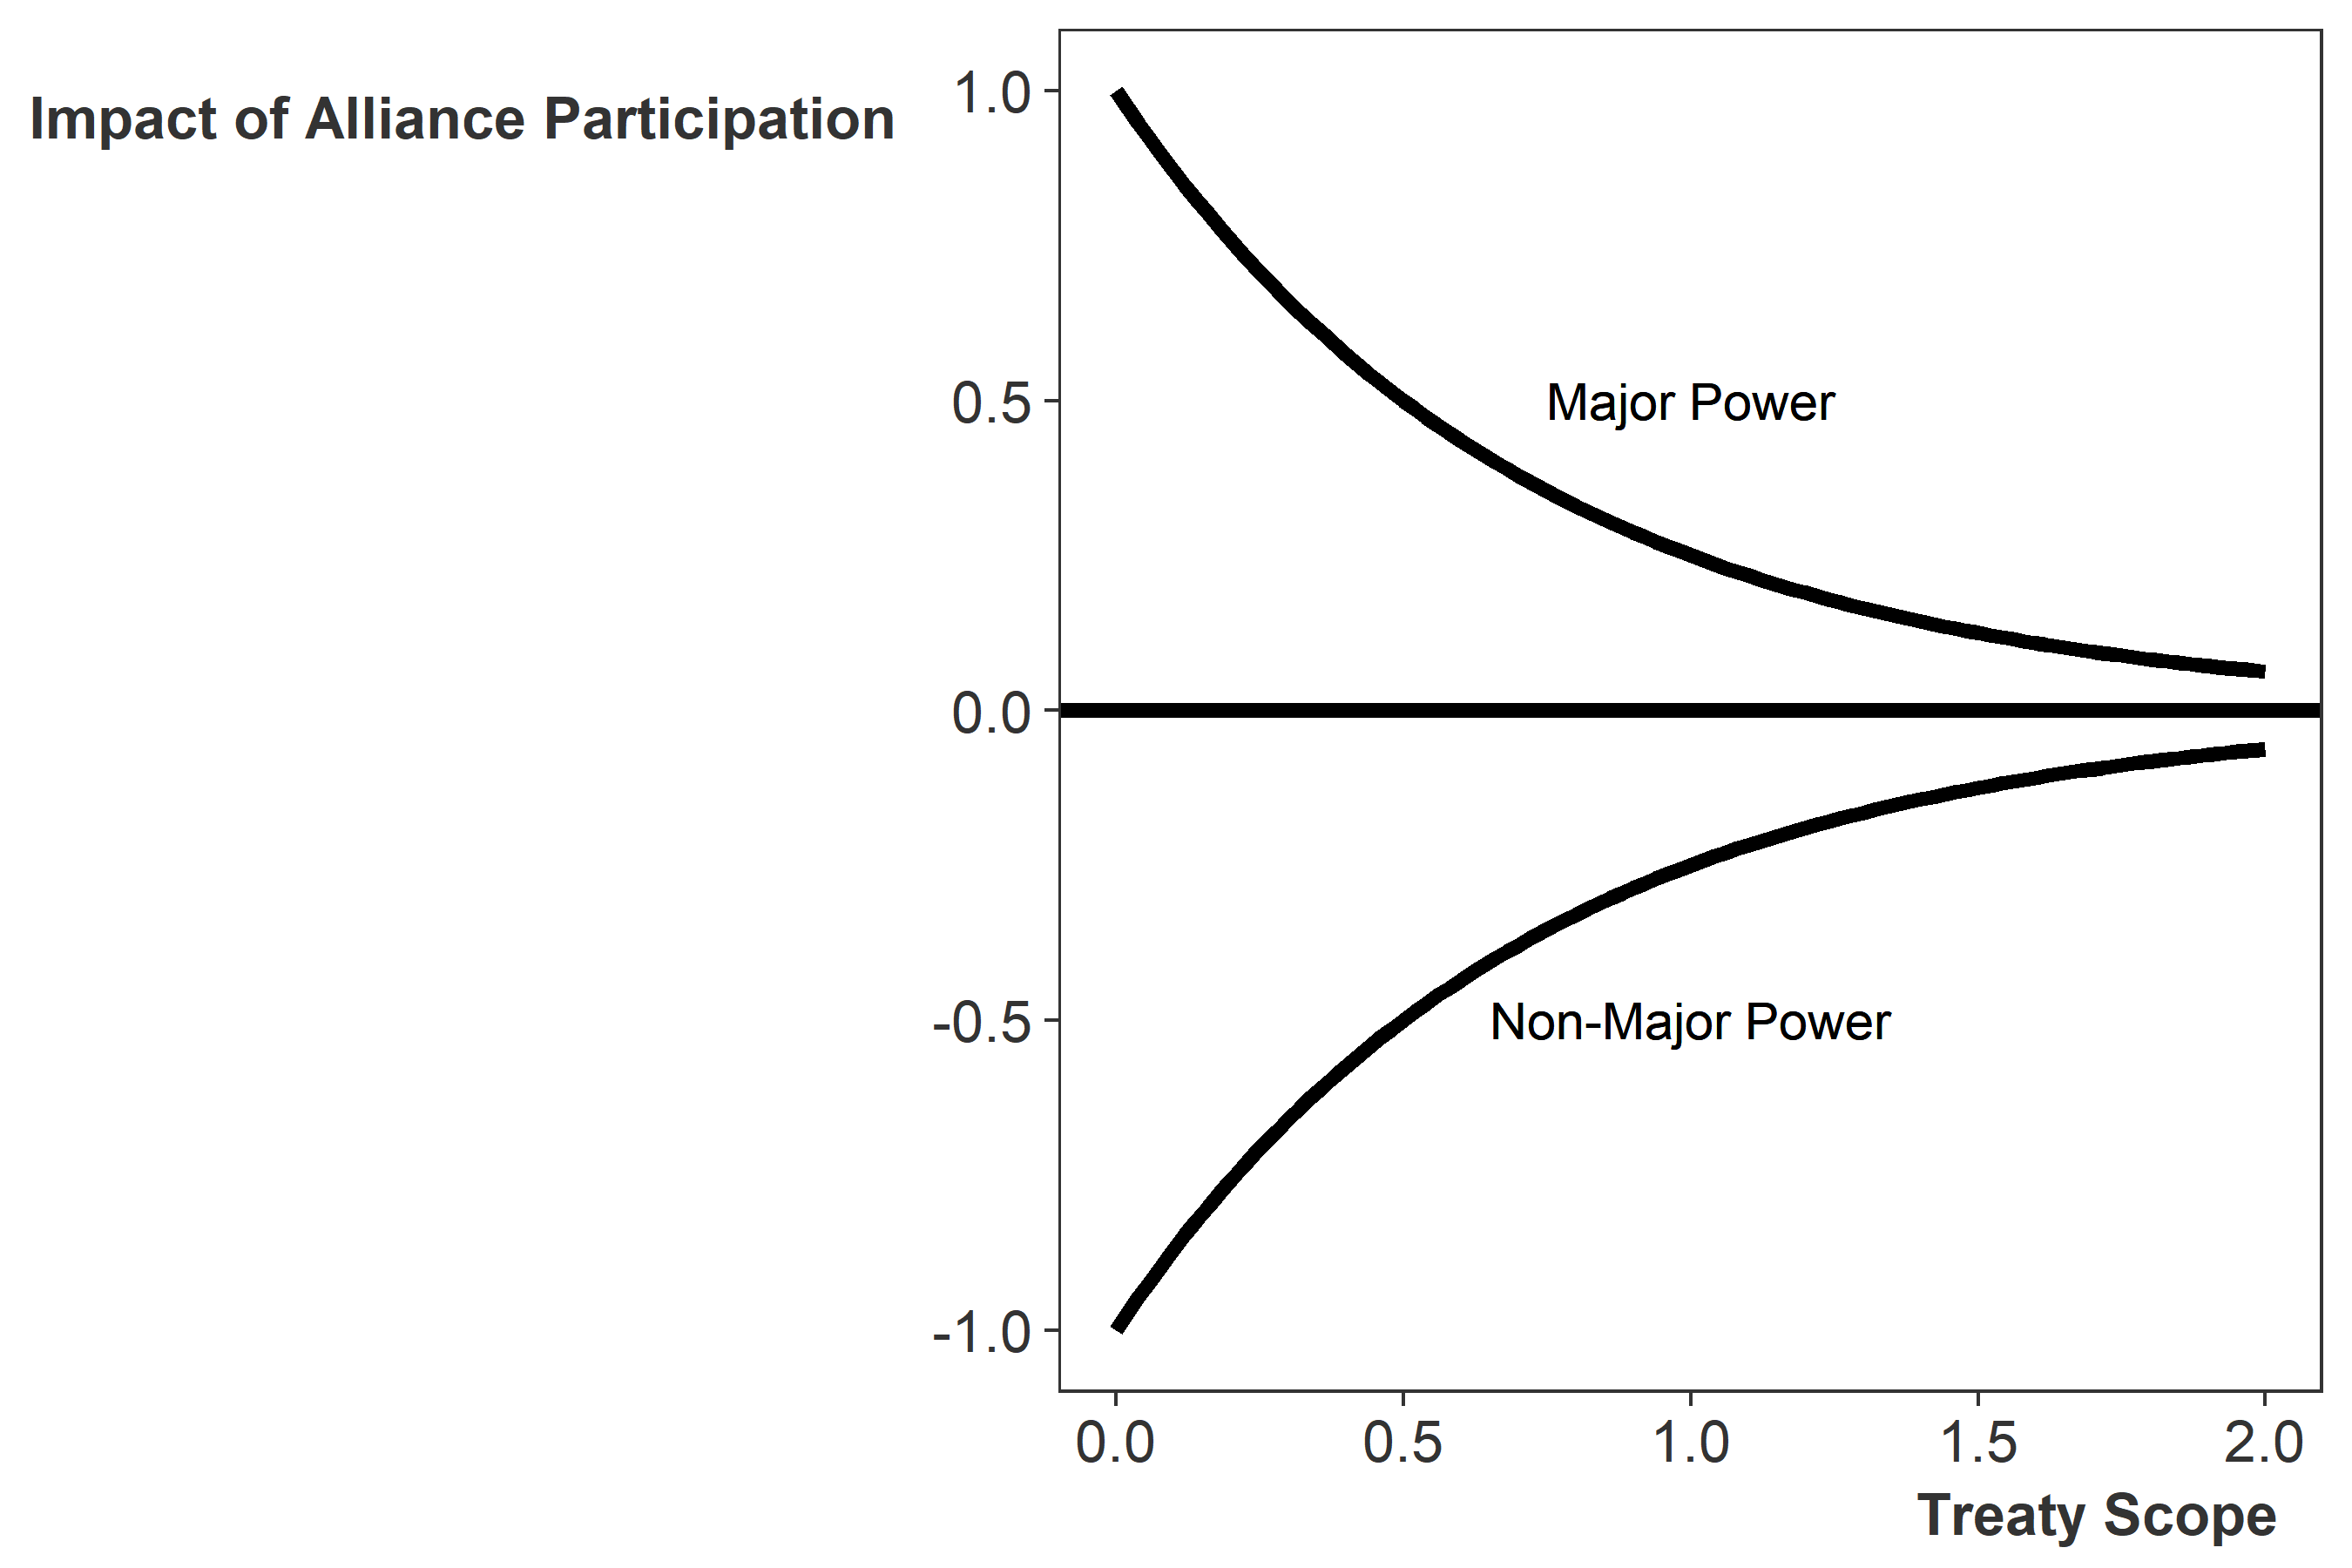
\includegraphics[width=0.95\textwidth]{illus-arg.png}
	\label{fig:illus-arg}
\end{figure}


\end{frame}


%-----------------------------------------------

\begin{frame}{Trace plots: Major}

\begin{figure}
	\centering
		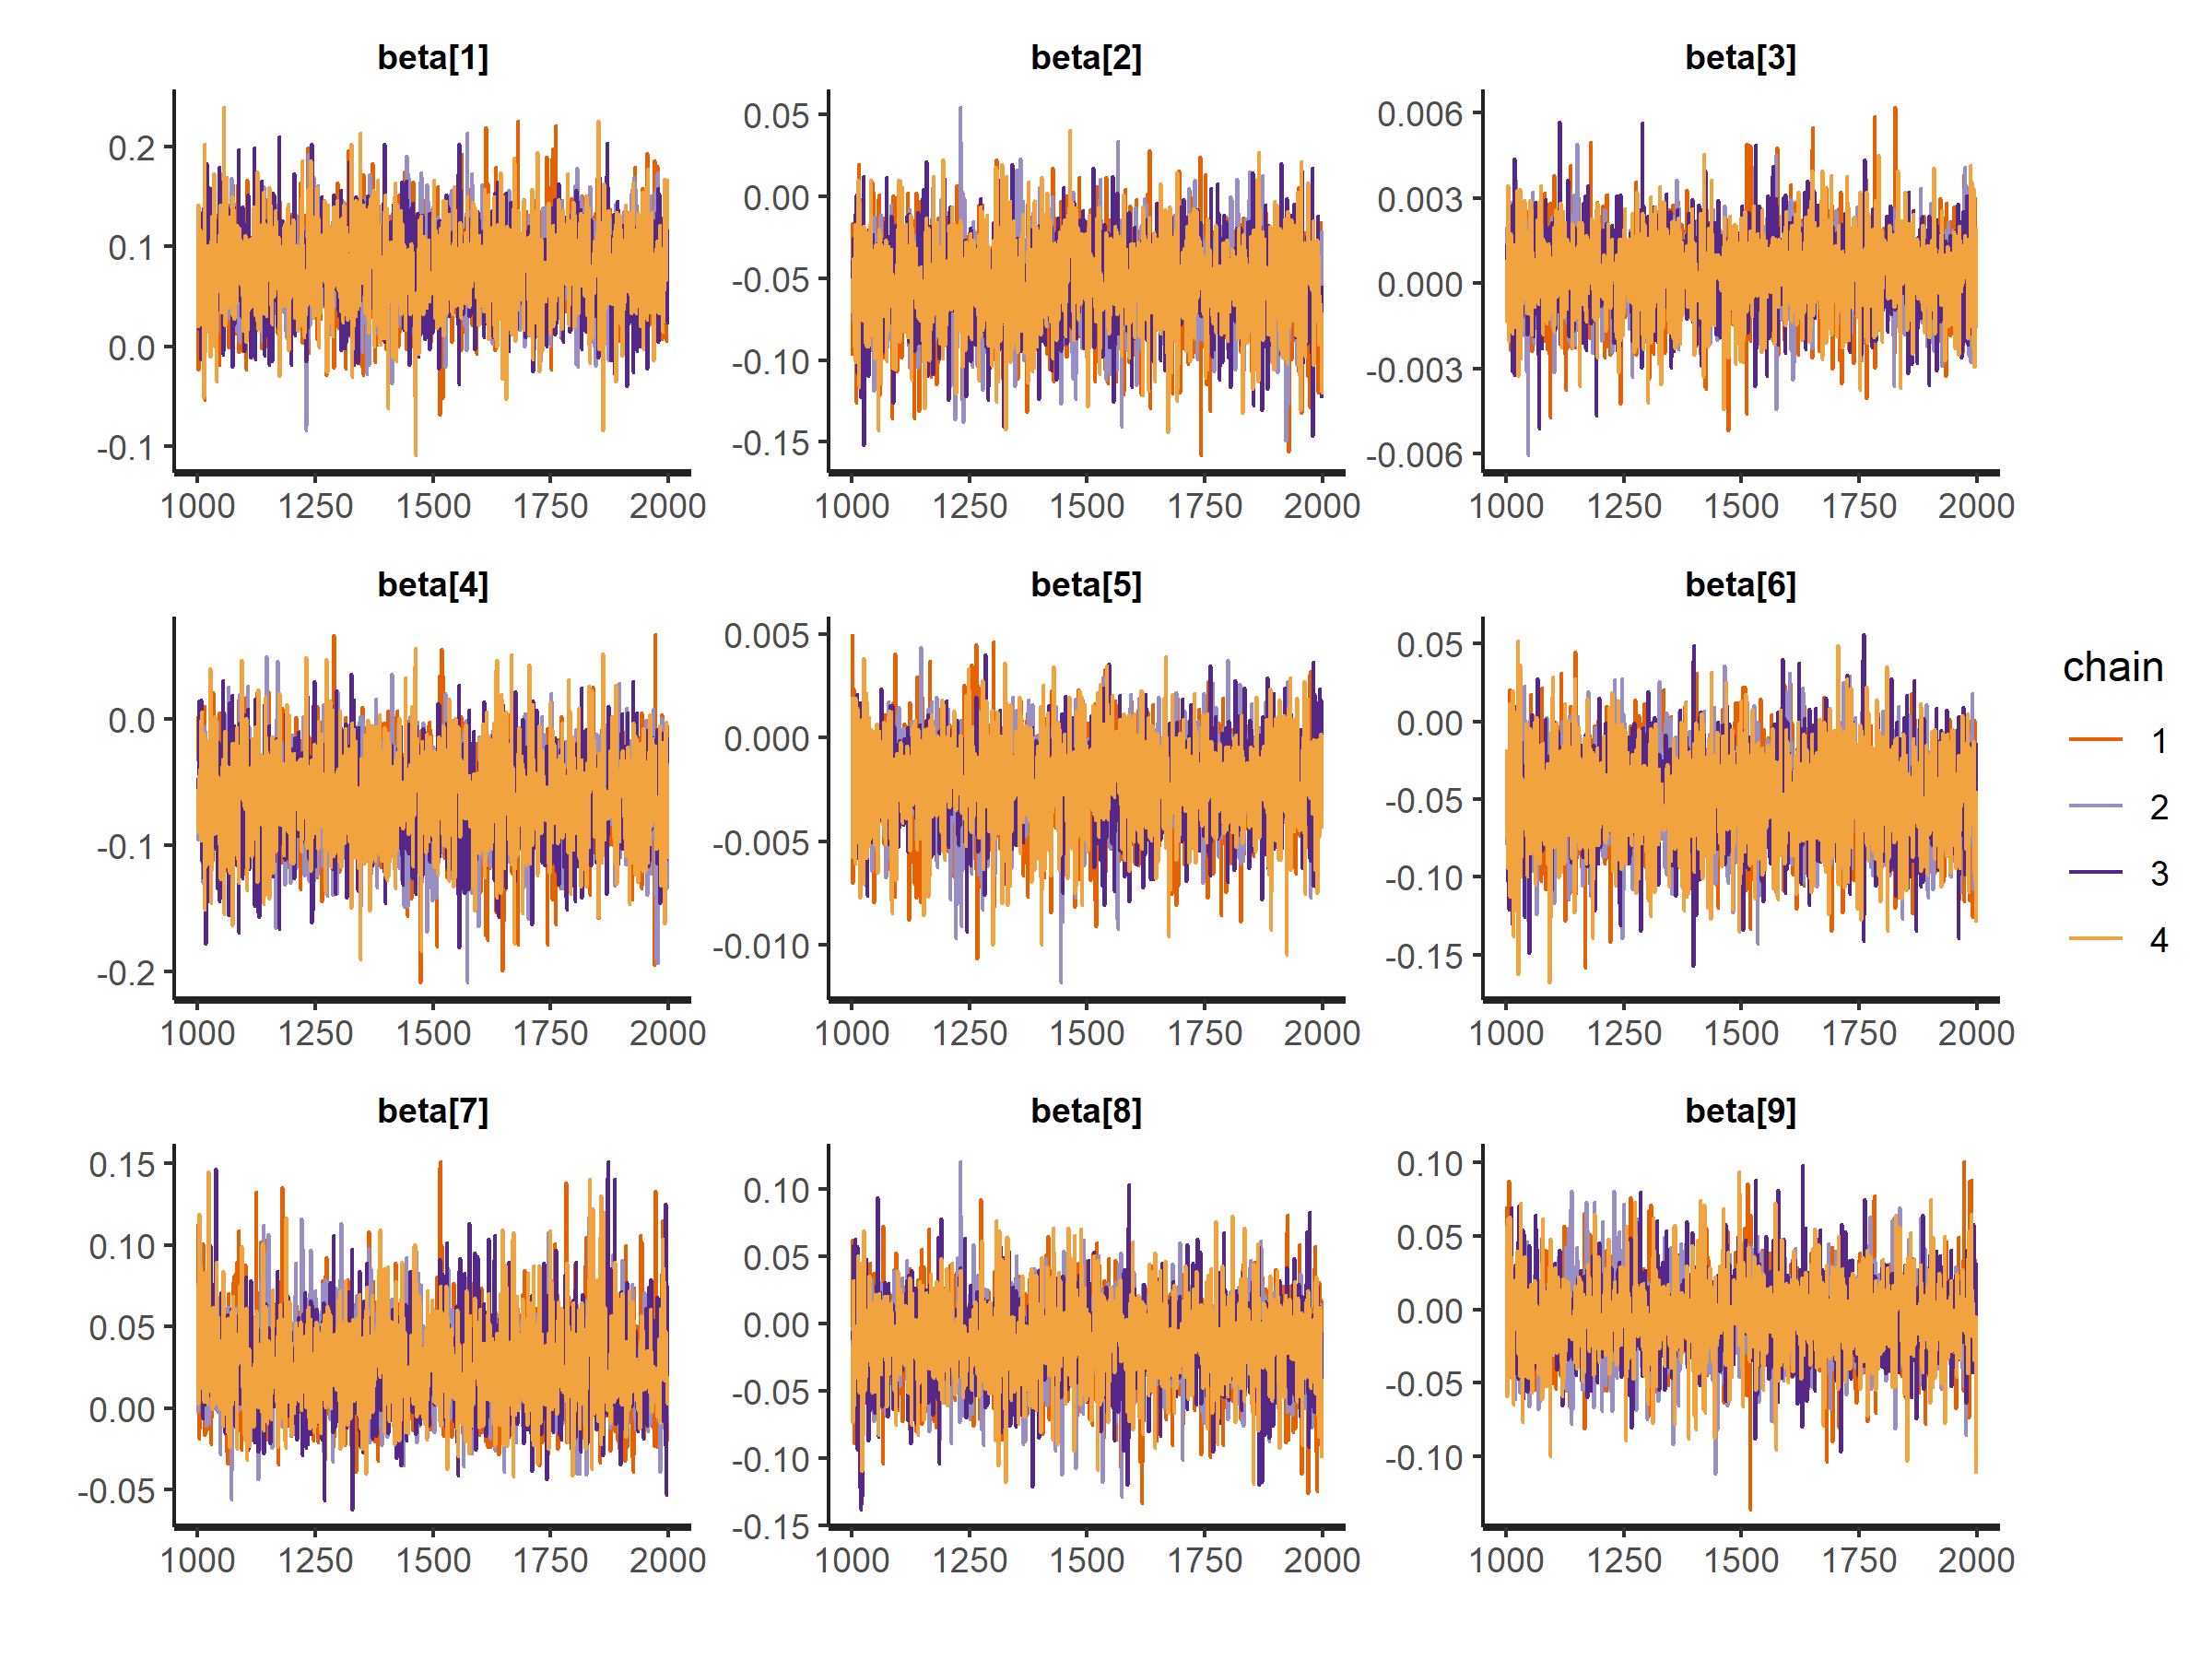
\includegraphics[width=0.95\textwidth]{beta-trace-maj.png}
\end{figure}


\end{frame}

%-----------------------------------------------

\begin{frame}{Trace plots: Non-Major}

\begin{figure}
	\centering
		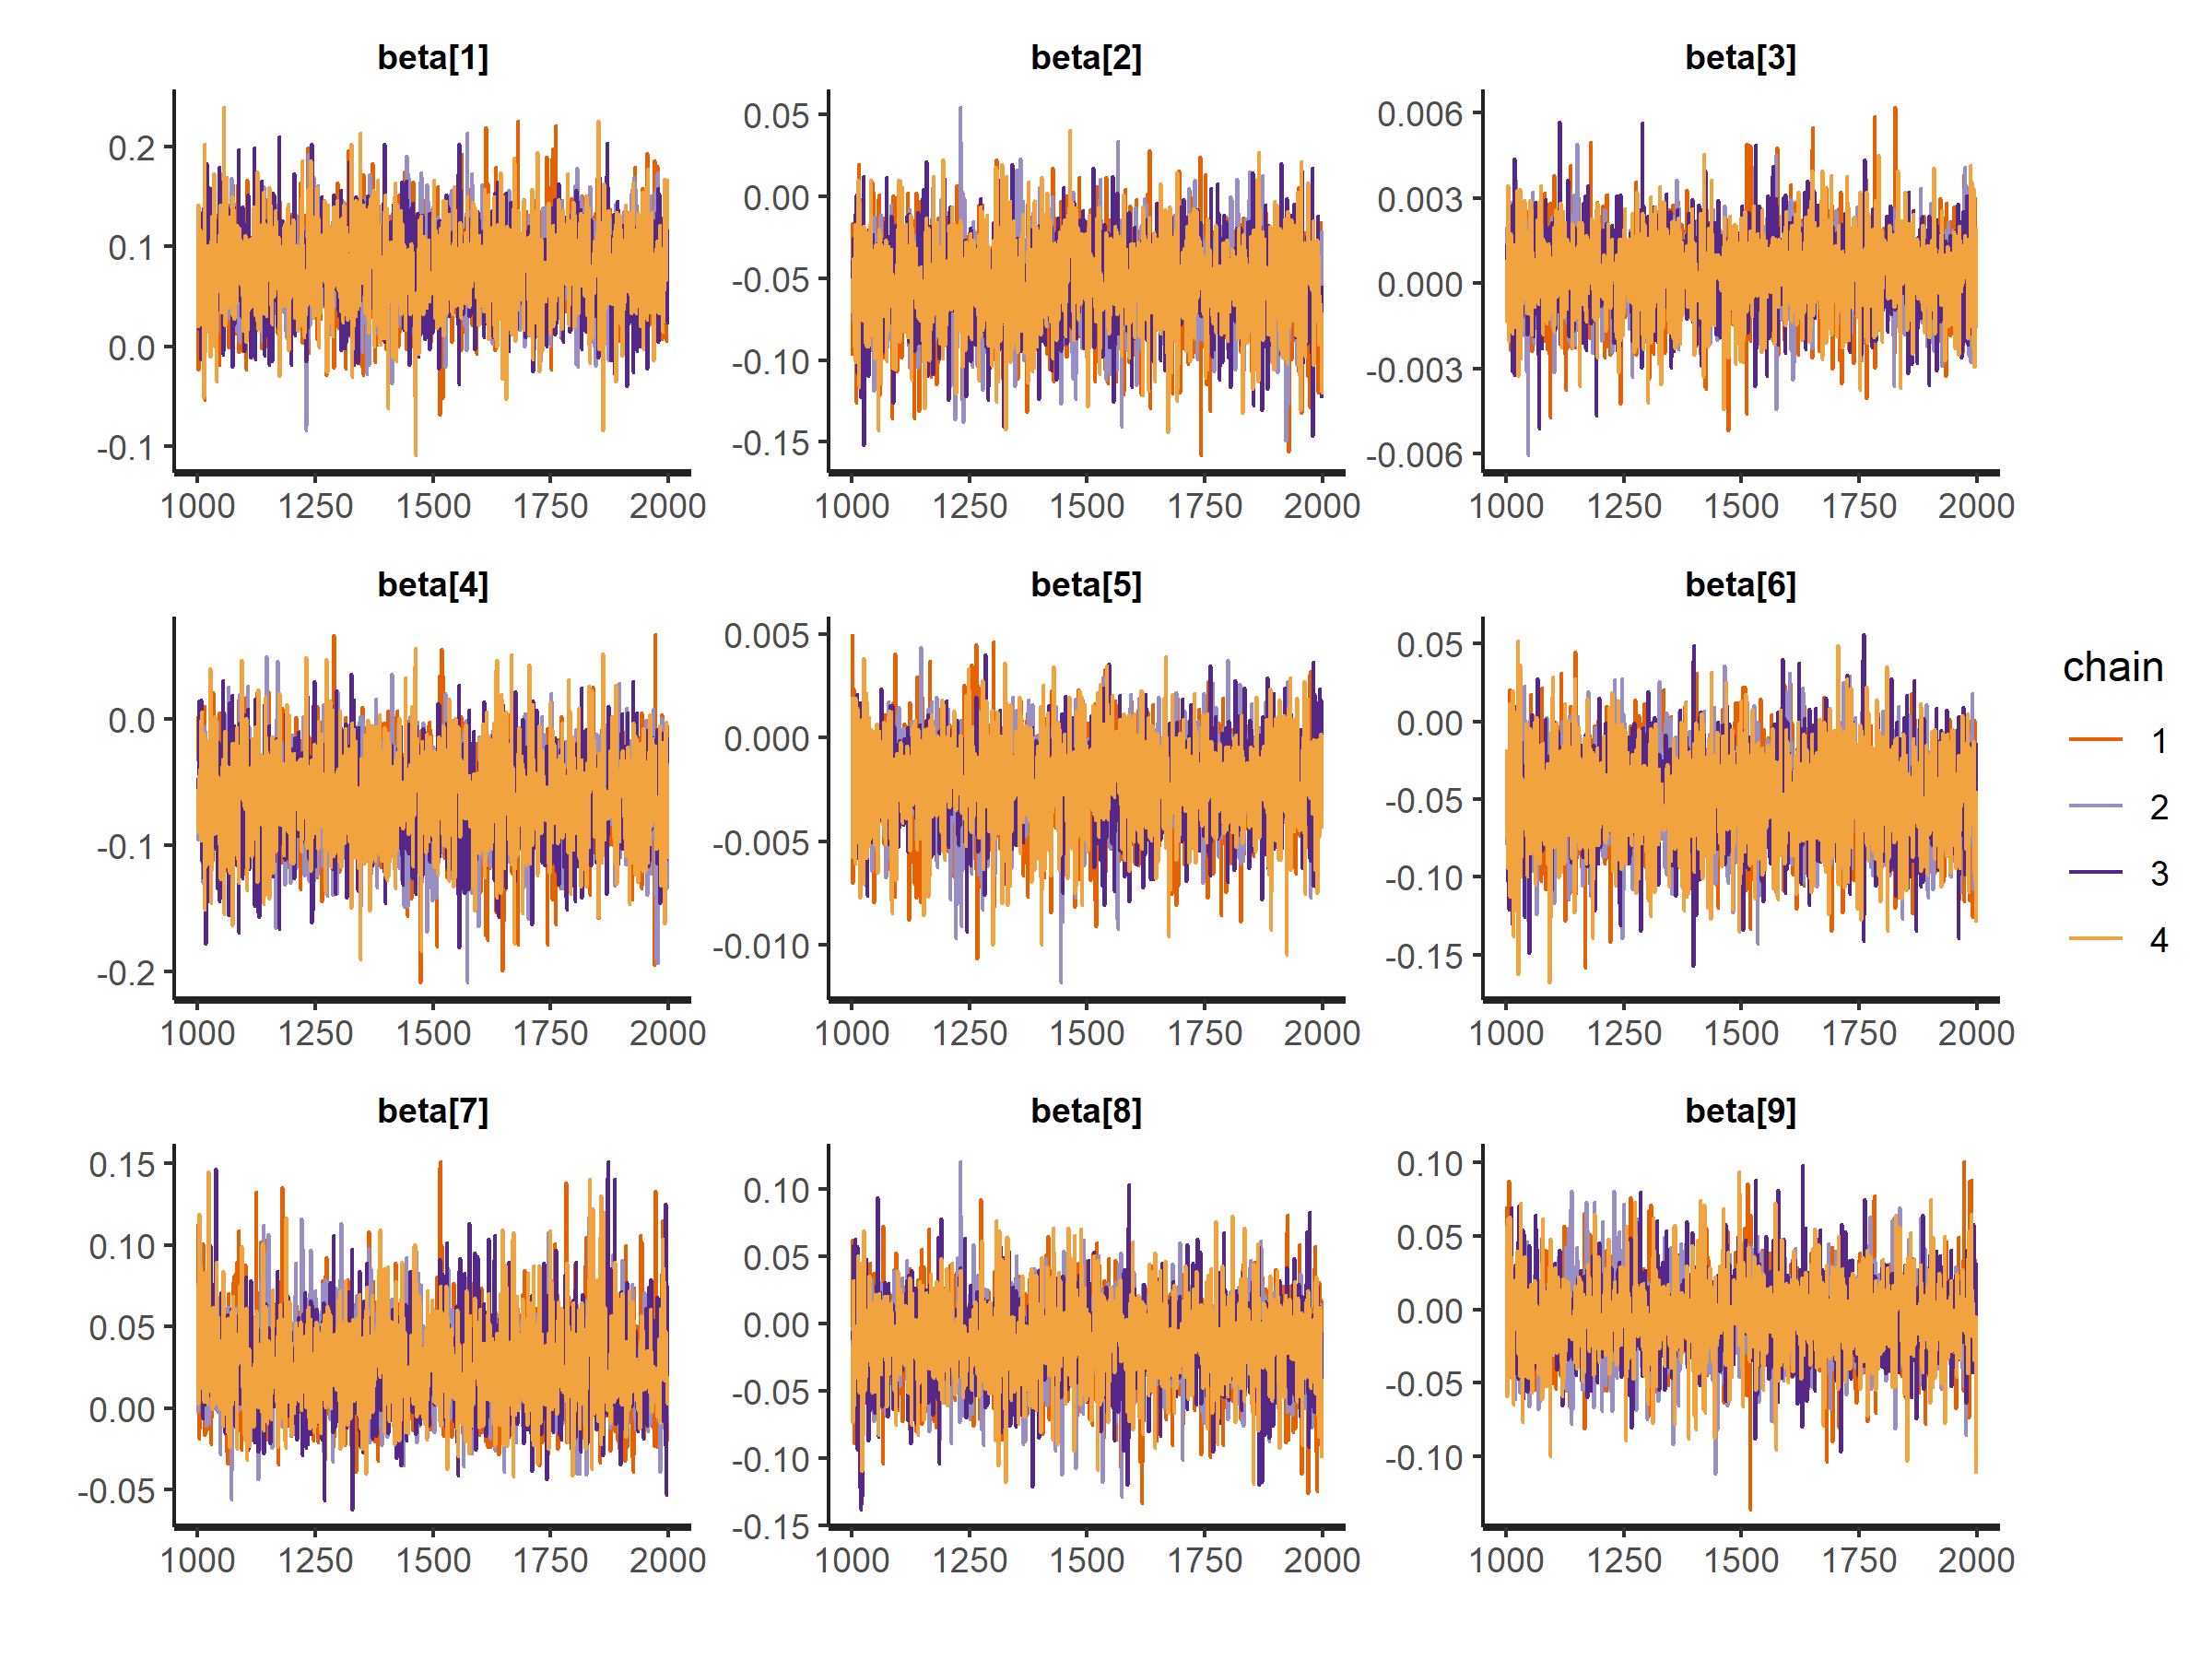
\includegraphics[width=0.95\textwidth]{beta-trace-maj.png}
\end{figure}


\end{frame}


%-----------------------------------------------

\begin{frame}{Model Check: Recovering Known Parameters}

Another way to check complicated models is simulating fake data with known parameters, then using the model to recover said parameters. 

To check my model, I simulated a fake dataset of 2,000 observations with 50 states, 200 years, 100 alliances and 2 variables at each level.

The 90\% credible intervals contain the known value for all regression parameters. 93 of 100 alliance specific parameter intervals contain the known value. 

\end{frame}


%-----------------------------------------------

\begin{frame}{Simulated Parameters and Credible Intervals}


\begin{figure}
	\centering
		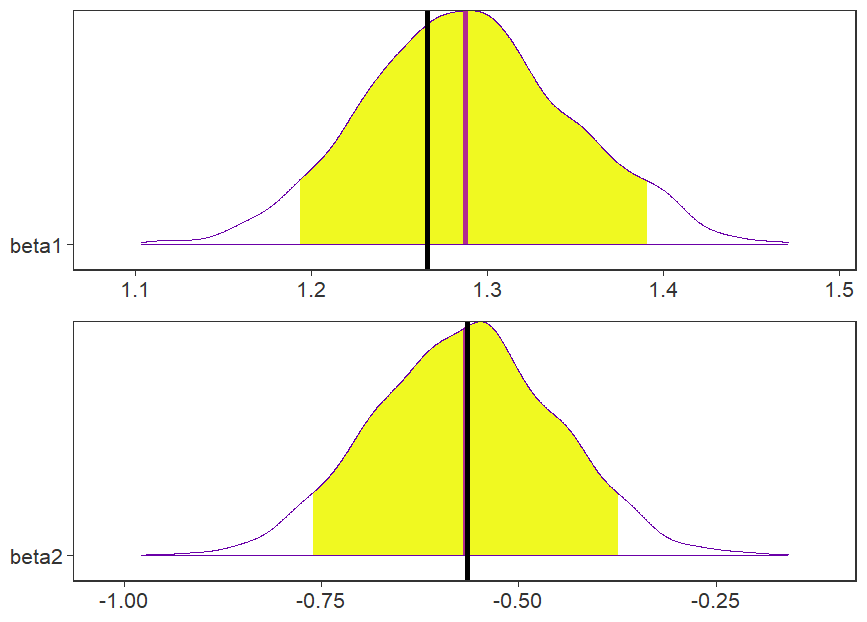
\includegraphics[width=0.95\textwidth]{sim-check-res.png}
\end{figure} 

\end{frame}


%------------------------------------------------


\begin{frame}{Alliance-Level Regression Table: Major Powers}

930 observations, with 130 alliances. 

\resizebox{.95\textwidth}{!}{
\begin{tabular}{rrrrrrr}
  \hline
 & mean & S.D. & 5\% & 95\% & n\_eff & $\hat{R}$ \\ 
  \hline
Constant & 0.038 & 0.038 & -0.025 & 0.102 & 3380.954 & 1.000 \\ 
  Latent Str. & -0.054 & 0.031 & -0.107 & -0.005 & 3278.923 & 1.000 \\ 
  Number Members & 0.000 & 0.002 & -0.003 & 0.003 & 4000.000 & 0.999 \\ 
  Democratic Membership & -0.009 & 0.033 & -0.065 & 0.042 & 4000.000 & 1.000 \\ 
  Wartime & -0.057 & 0.035 & -0.115 & -0.001 & 4000.000 & 1.001 \\ 
  Asymmetric & 0.053 & 0.035 & 0.001 & 0.115 & 2218.509 & 1.000 \\ 
  US Member & 0.002 & 0.031 & -0.051 & 0.051 & 4000.000 & 1.000 \\ 
  USSR Member & 0.023 & 0.033 & -0.028 & 0.079 & 4000.000 & 1.000 \\ 
  $\sigma$ Alliances & 0.066 & 0.029 & 0.019 & 0.117 & 599.081 & 1.007 \\ 
   \hline
\end{tabular}
}


\end{frame}

%-----------------------------------------------

\begin{frame}{Alliance-Level Regression Table: Non-Major Powers}

8,668 observations and 192 alliances. 

\resizebox{.95\textwidth}{!}{
\begin{tabular}{rrrrrrr}
  \hline
 & mean & sd & 5\% & 95\% & n\_eff & $\hat{R}$ \\ 
  \hline
Constant & -0.018 & 0.018 & -0.047 & 0.012 & 2211.374 & 1.000 \\ 
  Latent Str. & 0.026 & 0.017 & -0.002 & 0.054 & 2191.382 & 1.000 \\ 
  Number Members & 0.000 & 0.001 & -0.001 & 0.001 & 4000.000 & 1.000 \\ 
  Democratic Membership & -0.031 & 0.015 & -0.056 & -0.009 & 3213.621 & 1.000 \\ 
  Wartime & 0.041 & 0.023 & 0.002 & 0.078 & 4000.000 & 1.000 \\ 
  Asymmetric & -0.031 & 0.021 & -0.065 & 0.003 & 4000.000 & 0.999 \\ 
  US Member & 0.013 & 0.018 & -0.016 & 0.042 & 2895.419 & 1.000 \\ 
  USSR Member & 0.011 & 0.031 & -0.041 & 0.062 & 4000.000 & 1.000 \\ 
  $\sigma$ Alliances & 0.014 & 0.009 & 0.002 & 0.030 & 1254.268 & 1.001 \\ 
   \hline
\end{tabular}
}



\end{frame}


%------------------------------------------------


\begin{frame}{Priors}

4 Chains with 2,000 samples and 1,000 warmup iterations. 

\begin{table} % Create a table of priors.

 \begin{center}
\begin{tabular}{c} 
$ p(\alpha) \sim N(0, 1)$  \\
$ p(\sigma) \sim \mbox{half-}N(0, 1) $ \\
$ p(\alpha^{yr}) \sim N(0, \sigma^{yr}) $ \\ 
$ p(\sigma^{yr}) \sim N(0, 1) $ \\
$ p(\alpha^{st}) \sim N(0, \sigma^{st}) $ \\ 
$ p(\sigma^{st}) \sim \mbox{half-}N(0, 1) $ \\ 
$ p(\sigma^{all}) \sim \mbox{half-}N(0, 1) $ \\
$ p(\beta) \sim N(0, 1) $ \\
$ p(\gamma) \sim N(0, 1) $ \\ 
$ p(\nu) \sim gamma(2, 0.1)$ 
\end{tabular} 
\end{center} 
\label{tab:priors}
\end{table} 


\end{frame}


%------------------------------------------------

\begin{frame}{Details of Measurement Model}

\begin{itemize}
\item Bayesian Gaussian Copula Factor Model: for mixed data. 
\item Uses copulas to break dependence between latent factors and marginal distributions. 
\item Treats marginals as unknown and keeps them free of dependence. 
\item IMH proposal, 10,000 iteration warmup, 20,000 samples, thinned every 20 draws. 
\item Generalized double Pareto prior for the factor loading--- flexible generalized Laplace distribution with a spike at zero and heavy tails. 
\end{itemize} 


\end{frame}


%------------------------------------------------

\begin{frame}{Notable Major Power Alliances}


\begin{figure}
	\centering
		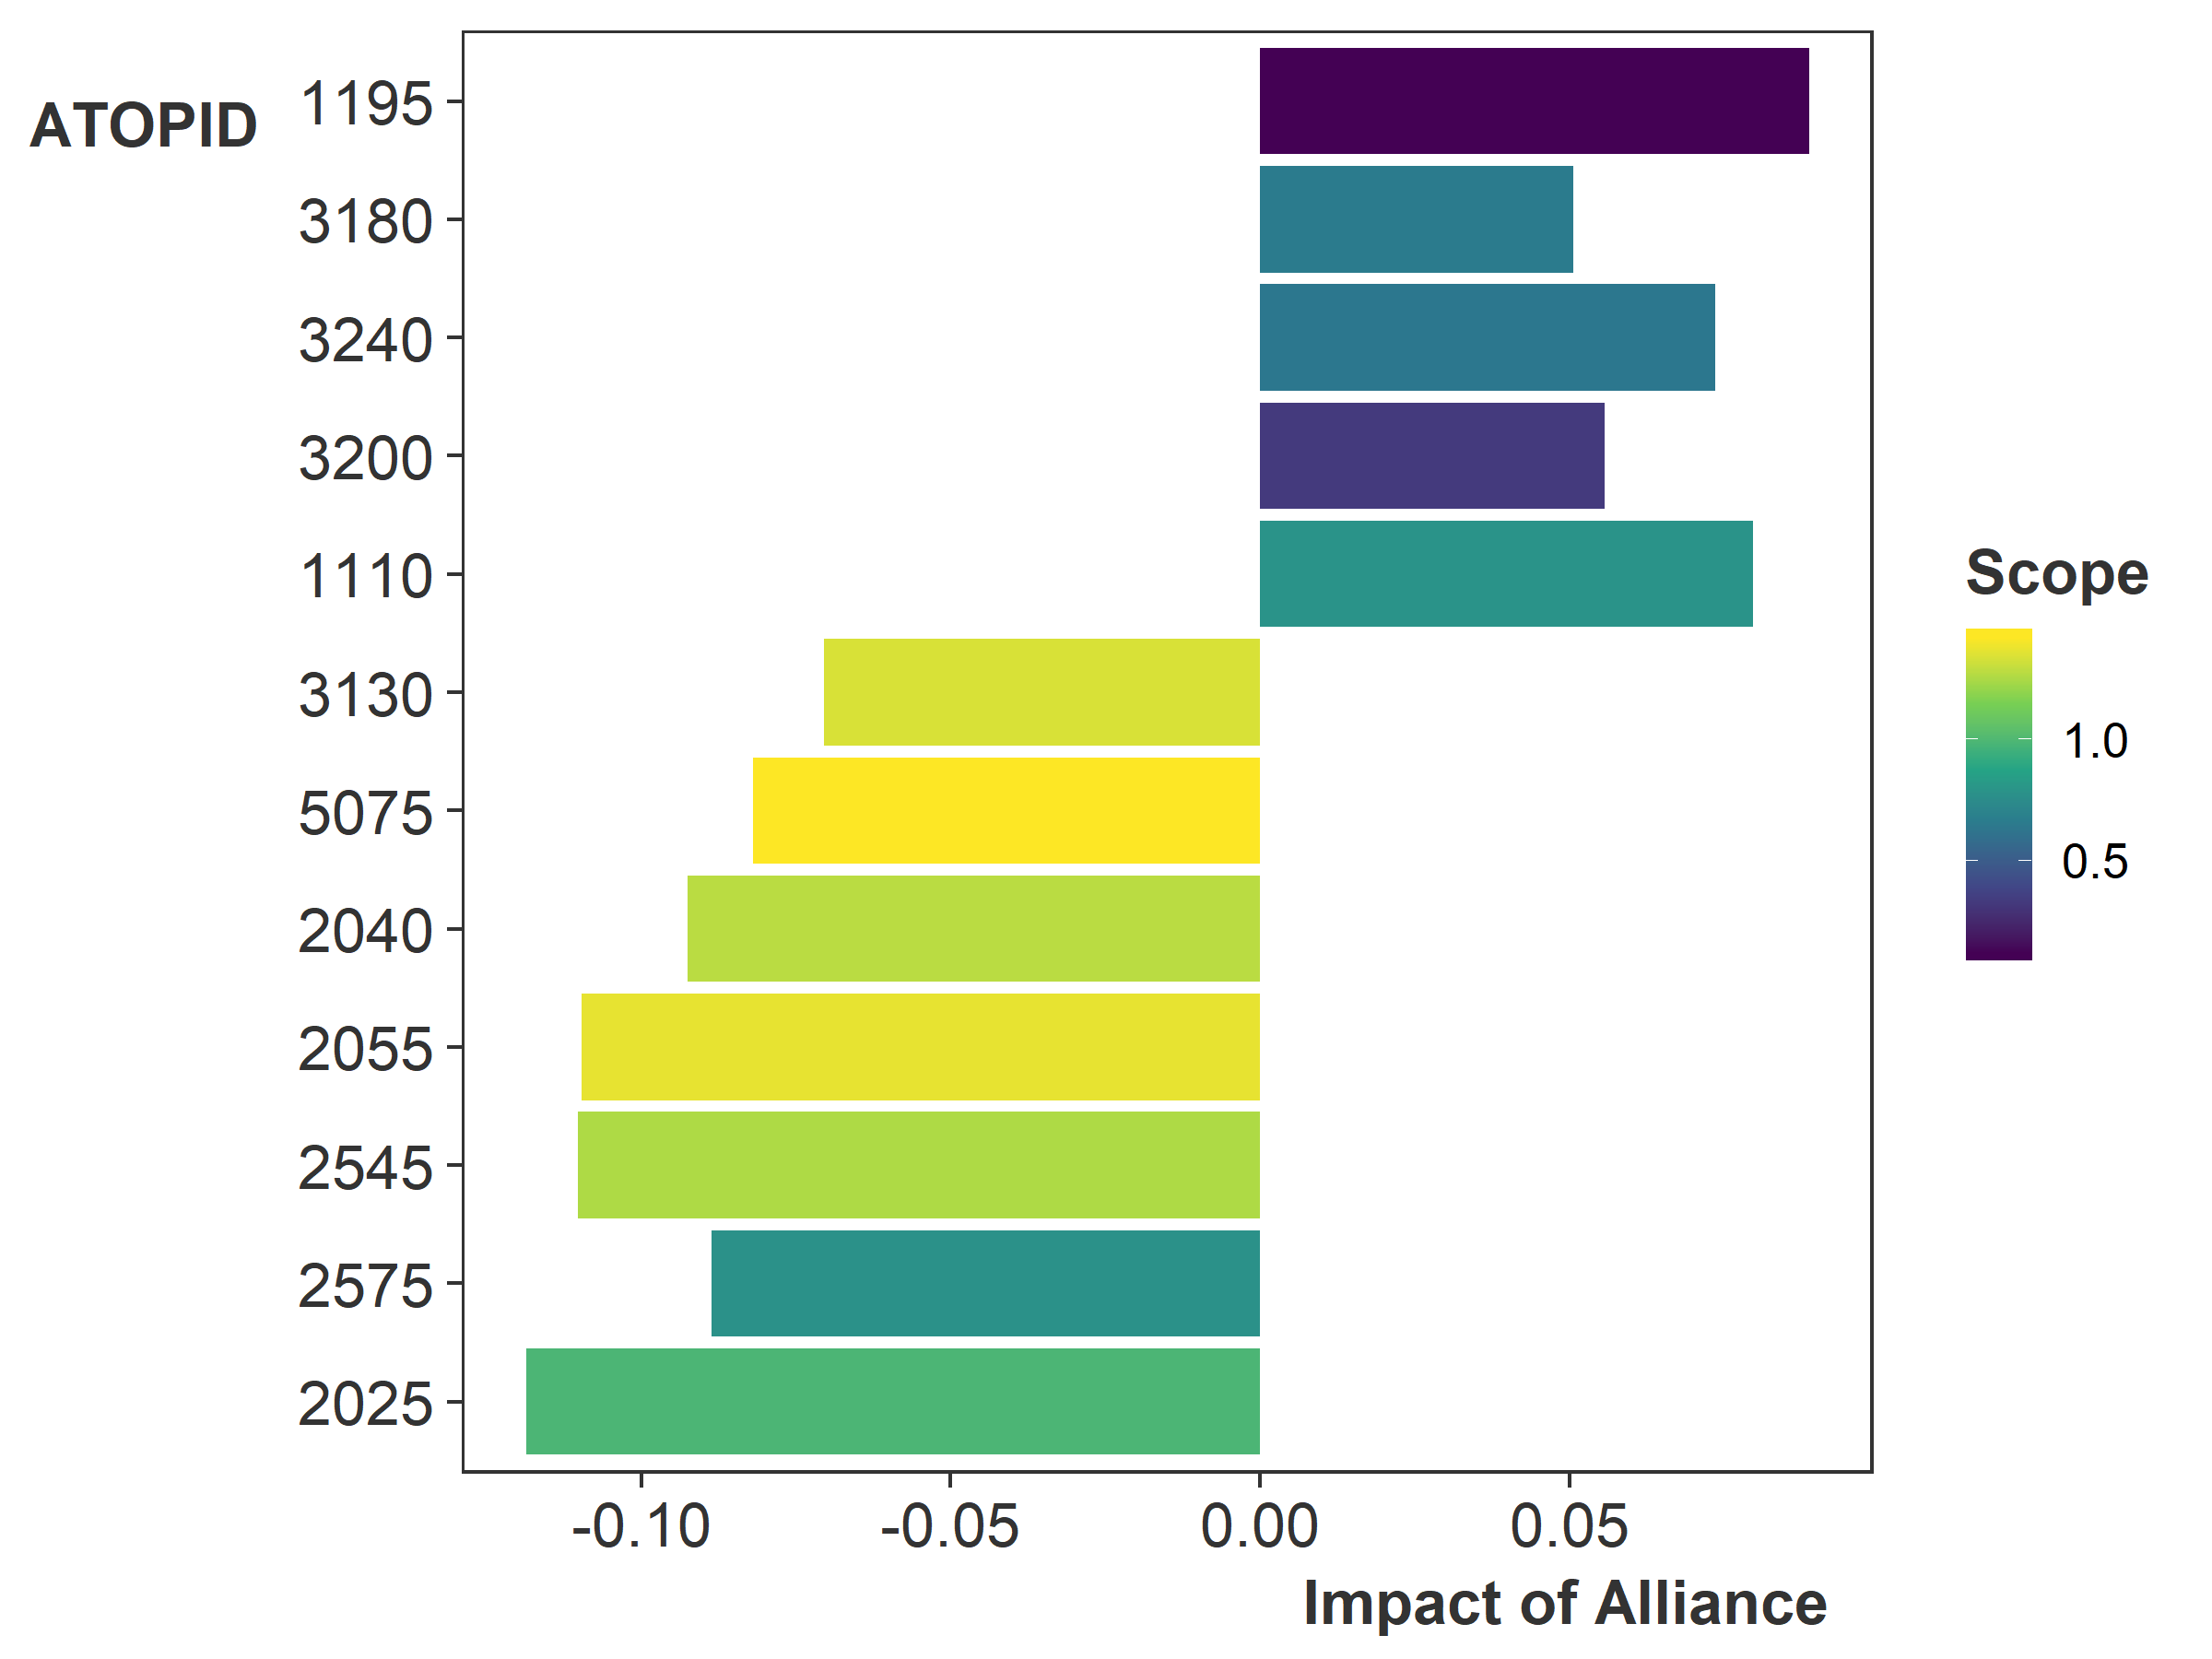
\includegraphics[width=0.95\textwidth]{non-zero-maj.png}
	\label{fig:non-zero-maj}
\end{figure}


\end{frame}

%------------------------------------------------

\begin{frame}{Notable Non-Major Power Alliances}


\begin{figure}
	\centering
		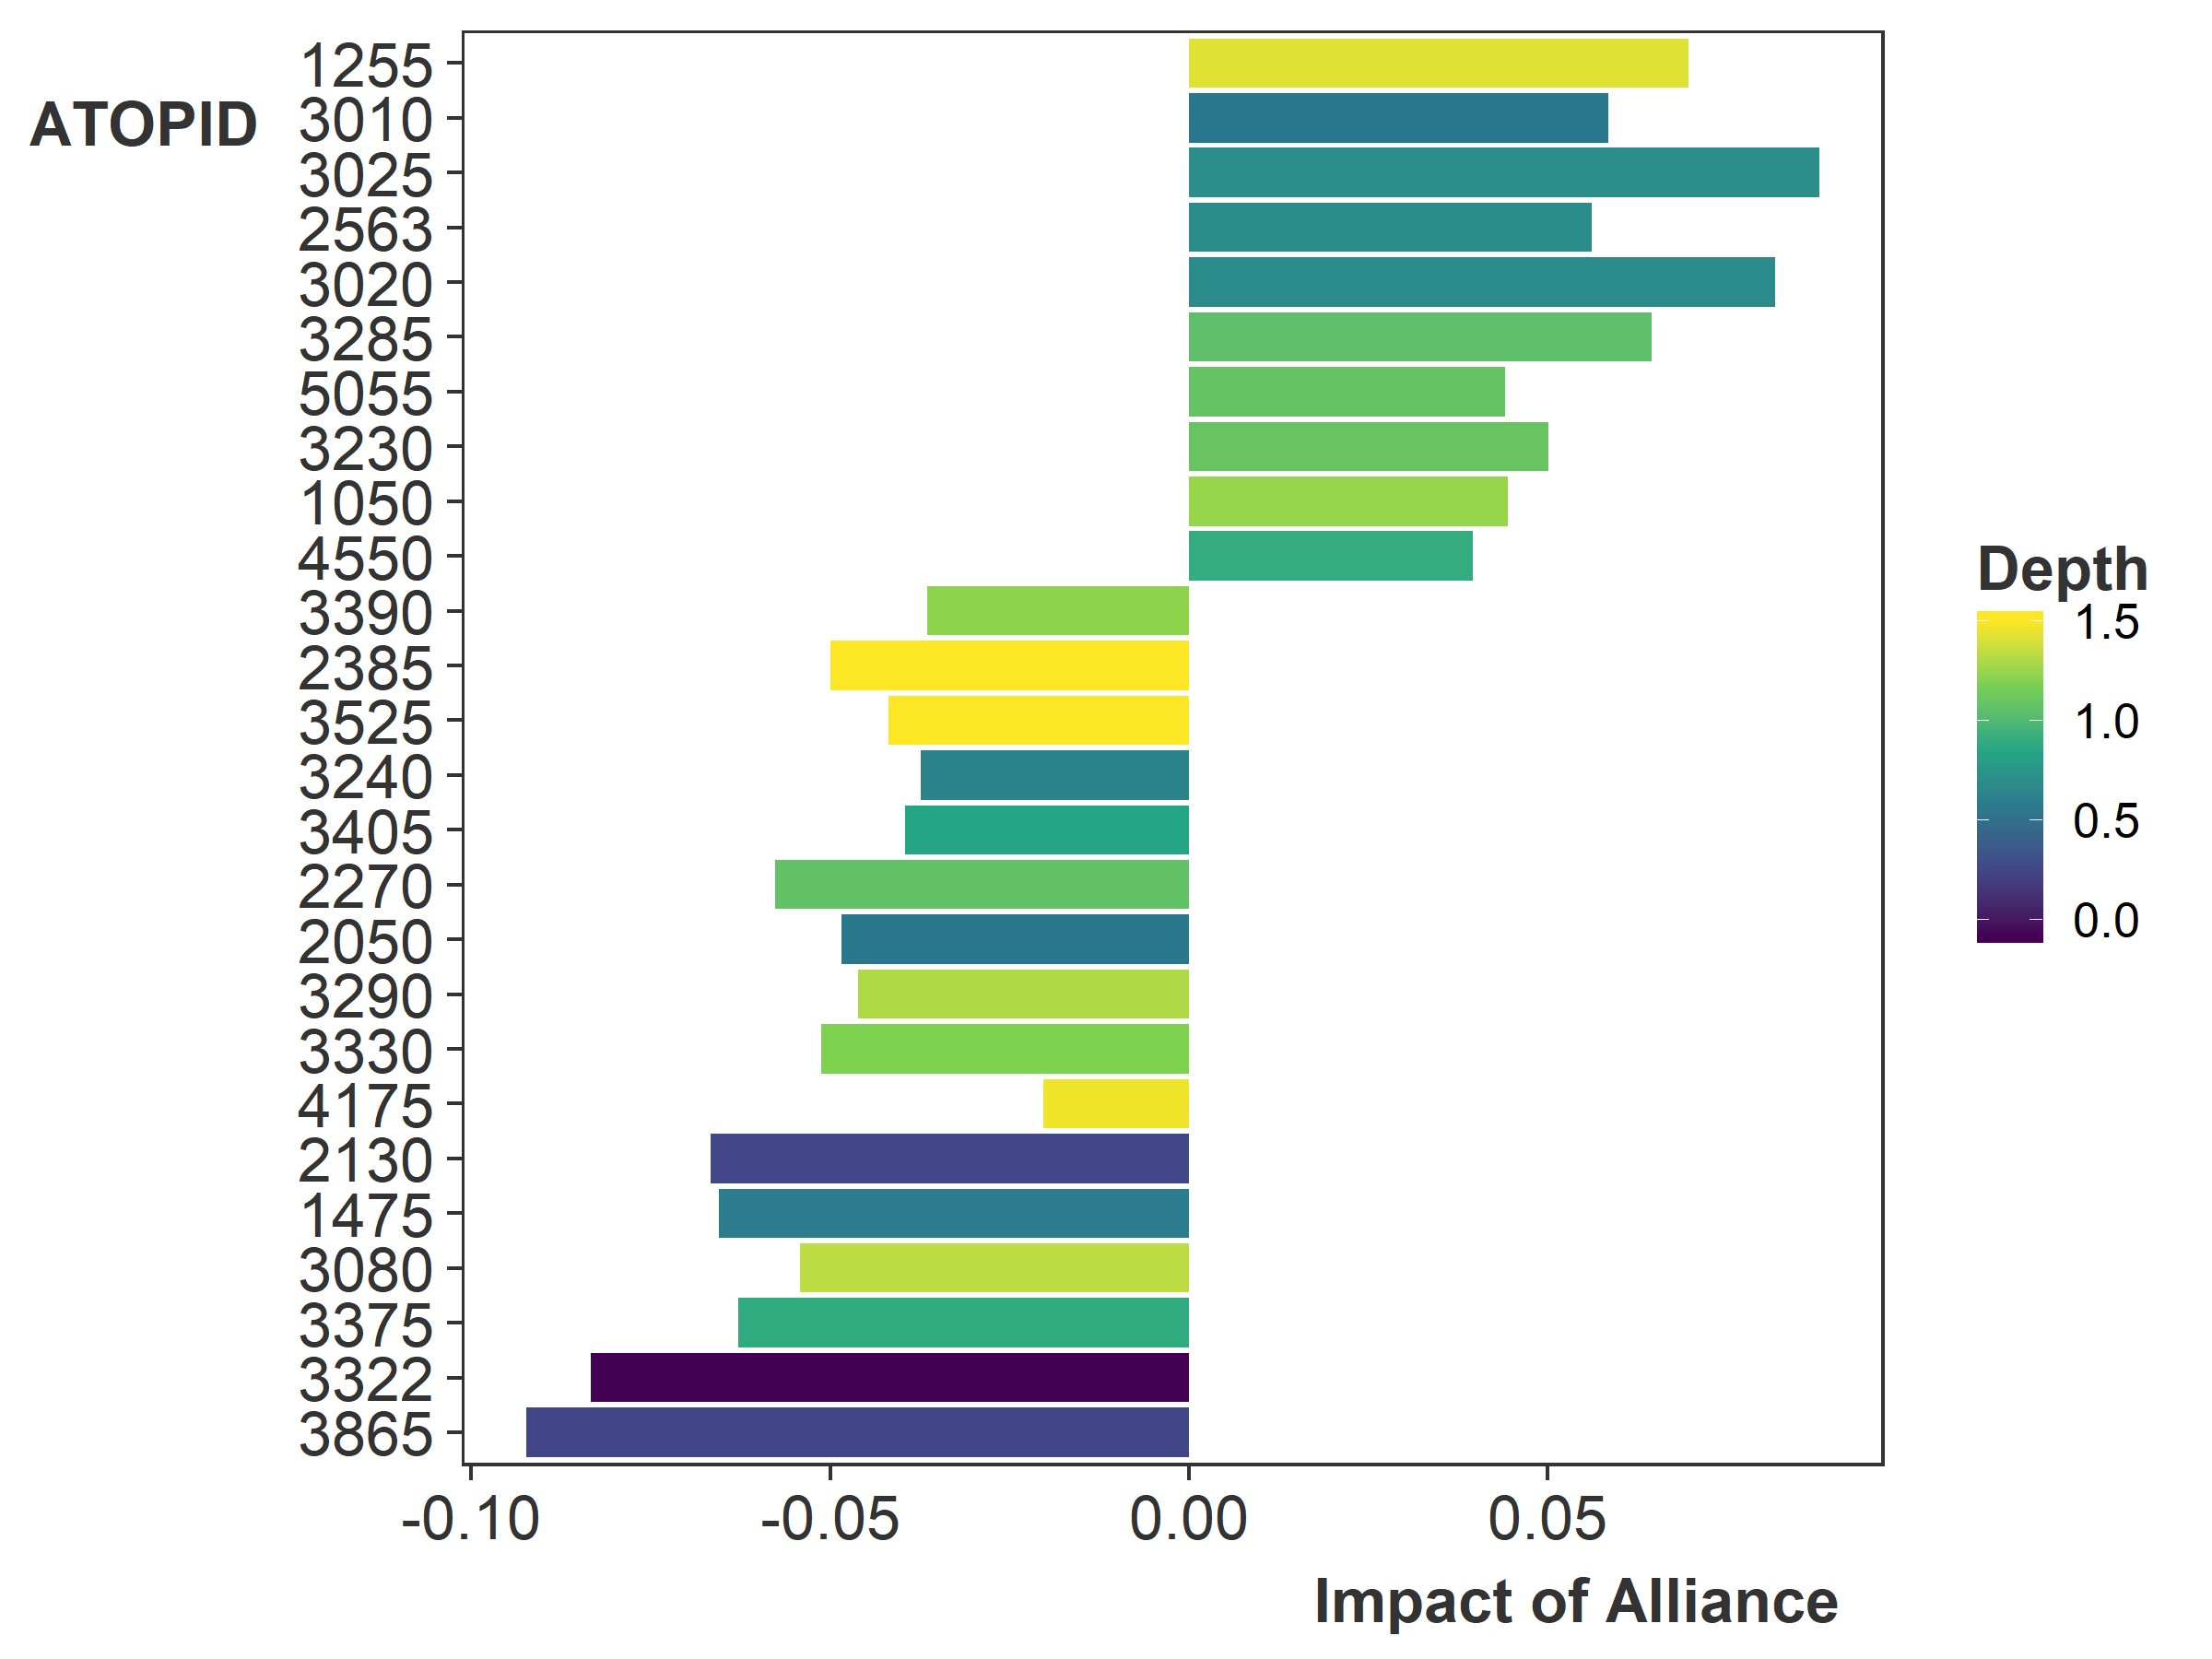
\includegraphics[width=0.95\textwidth]{non-zero-min.png}
	\label{fig:non-zero-min}
\end{figure}


\end{frame}


%------------------------------------------------

\begin{frame}{Non-Major Powers in NATO: Belgium}


\begin{figure}
	\centering
		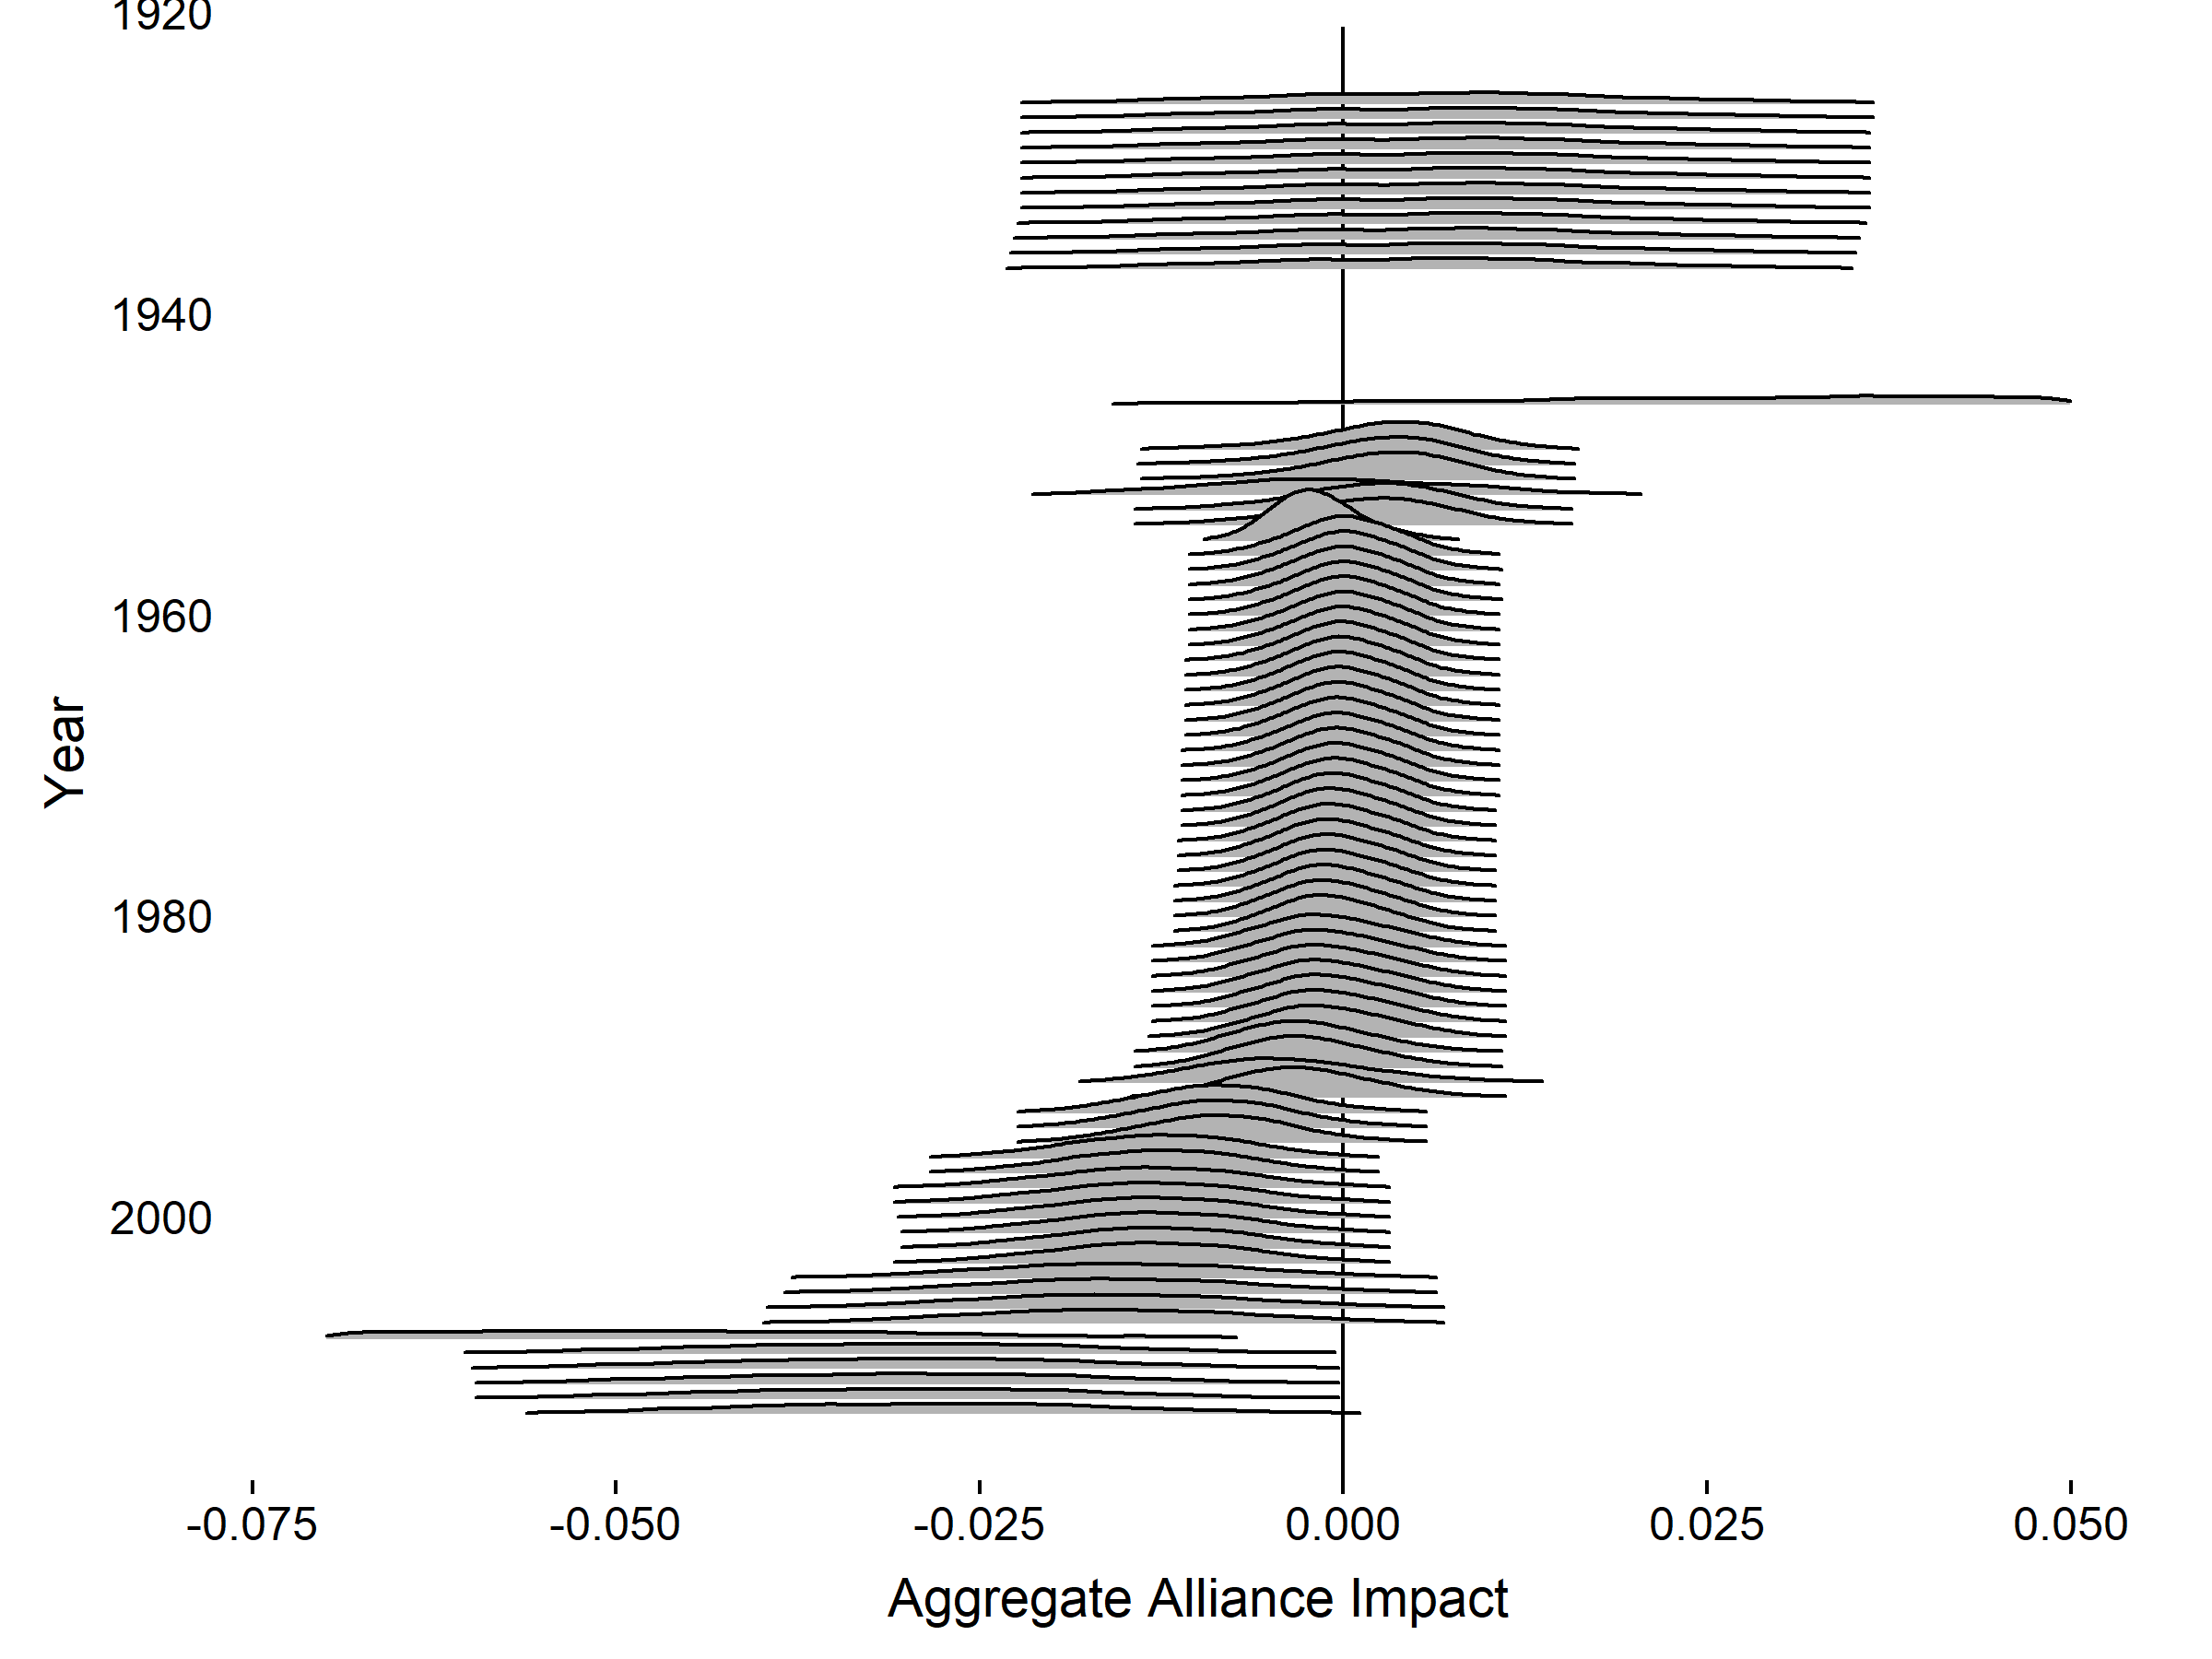
\includegraphics[width=0.95\textwidth]{bel-agg-imp.png}
\end{figure}


\end{frame}


%------------------------------------------------

\begin{frame}{Impact of NATO on Belgium}


\begin{figure}
	\centering
		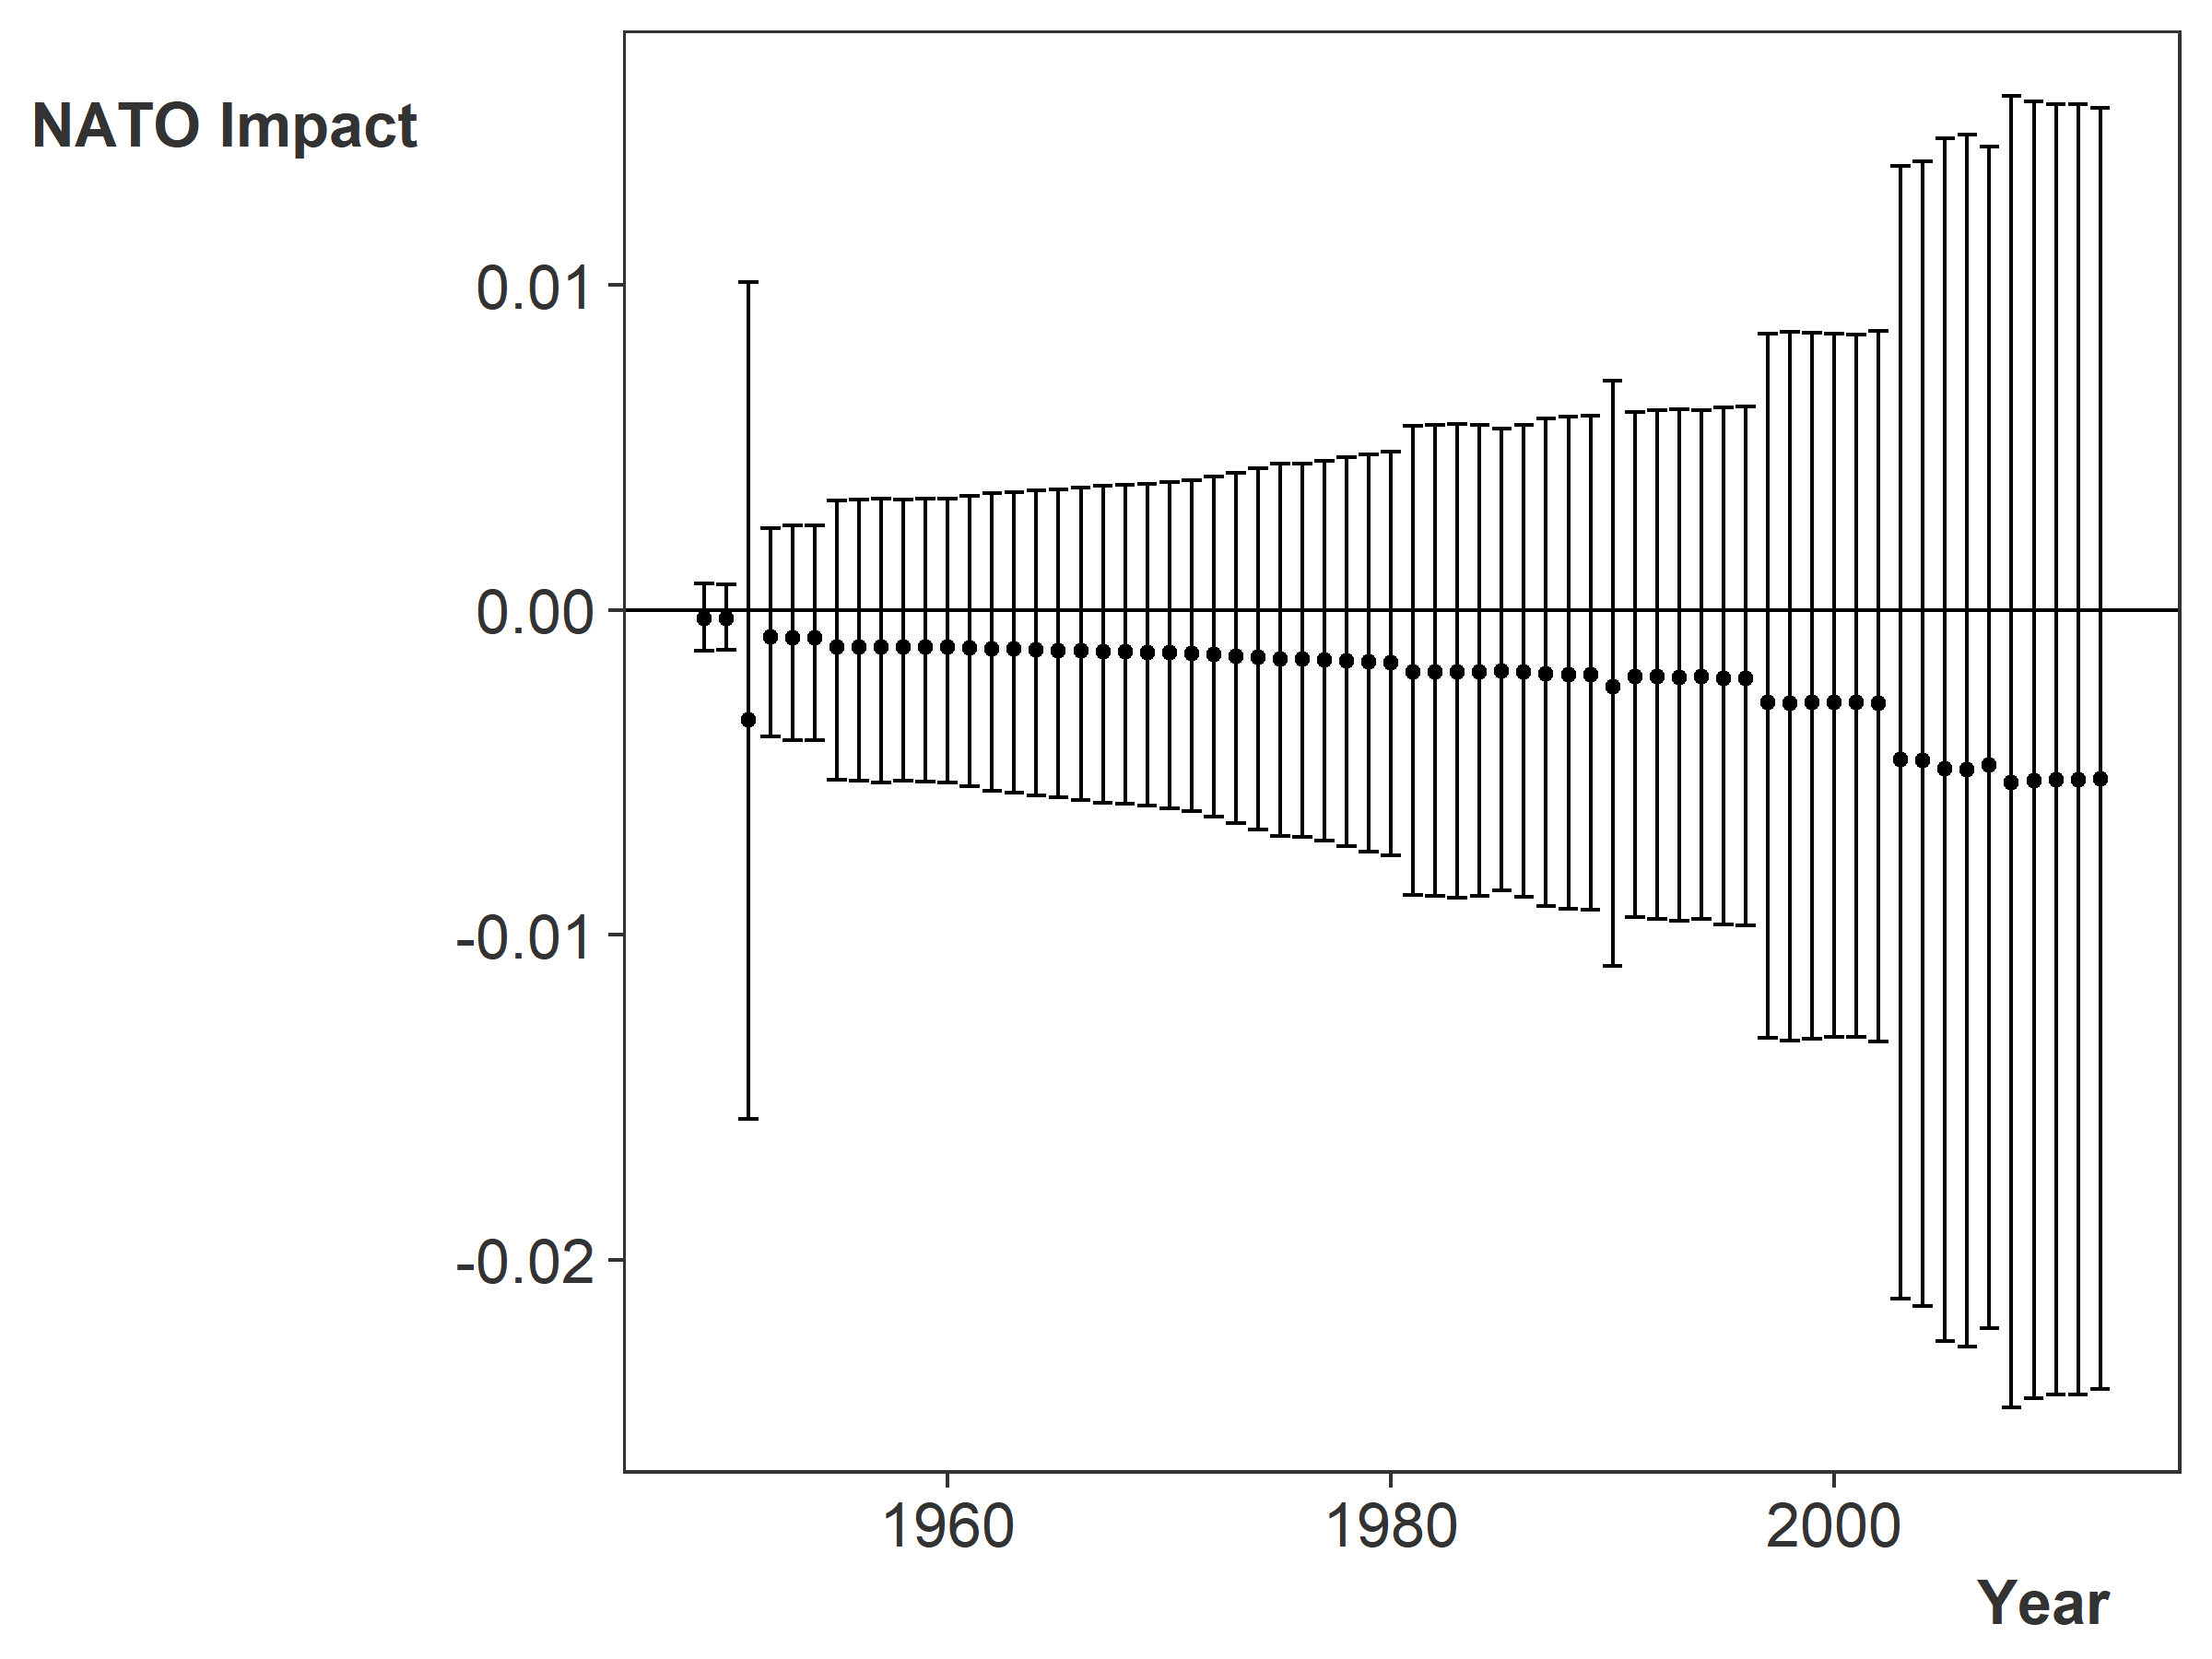
\includegraphics[width=0.95\textwidth]{bel-nato-imp.png}
\end{figure}


\end{frame}


%------------------------------------------------

\begin{frame}{Impact of EU on Belgium}


\begin{figure}
	\centering
		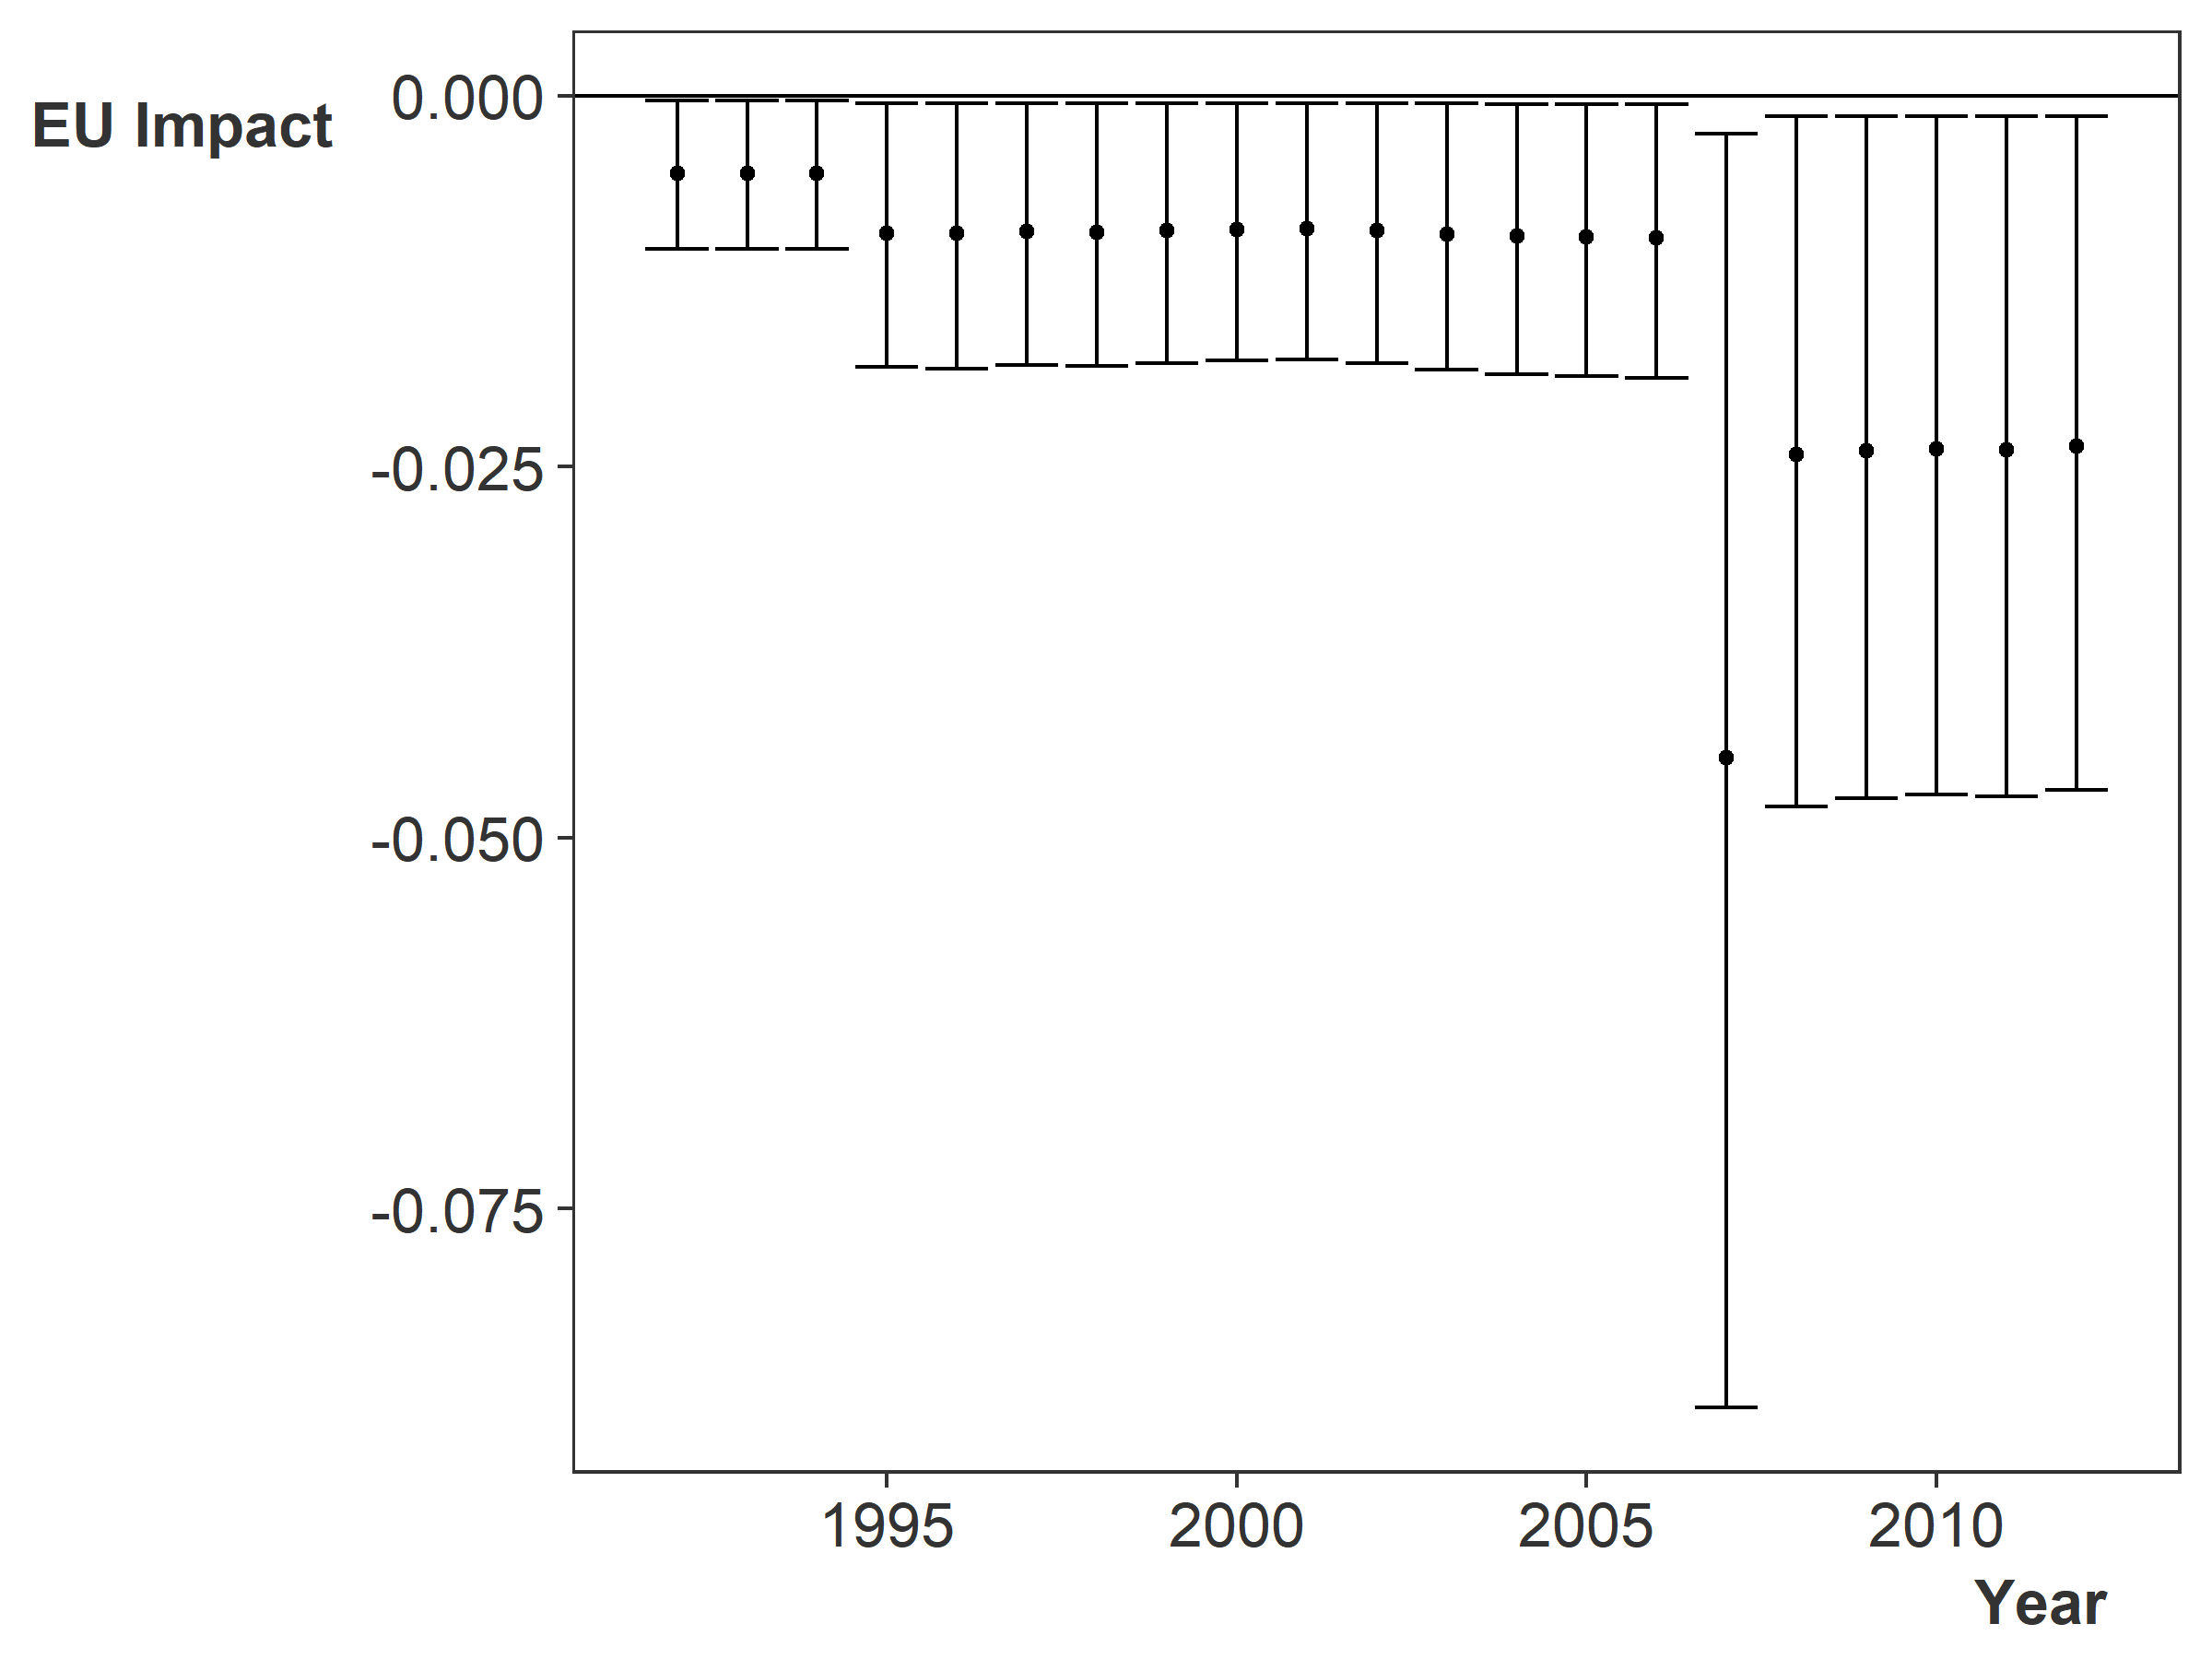
\includegraphics[width=0.95\textwidth]{bel-eu-imp.png}
\end{figure}


\end{frame}




%------------------------------------------------

\begin{frame}{Varying Slopes Model}

Within each of the $j$ groups of state capability, for $i$ in $1 ... n_j$: 
\begin{equation*}
y_i \sim student_t(\nu_j, \alpha_j + \alpha^{st} + \alpha^{yr} +\textbf{W}_{i} \gamma  + \textbf{Z}_{ji} \lambda_{j}, \sigma_j) 
\end{equation*} 

\begin{equation*}
\lambda_{j} \sim N(\theta_{j}, \sigma^{all}_{j})
\end{equation*} 

\begin{equation*}
\theta_{j} = \alpha^{all}_{j} + \textbf{X} \beta_j
\end{equation*}

I give $\beta_j$ a multivariate normal prior with prior scale $\tau$:
\begin{equation*}
\beta_j \sim MVN(\mu_{\beta_j}, \Sigma_{\beta}) 
\end{equation*}

\end{frame}


%------------------------------------------------

\begin{frame}{Varying Slopes Results: depth}

\begin{figure}[htbp]
	\centering
		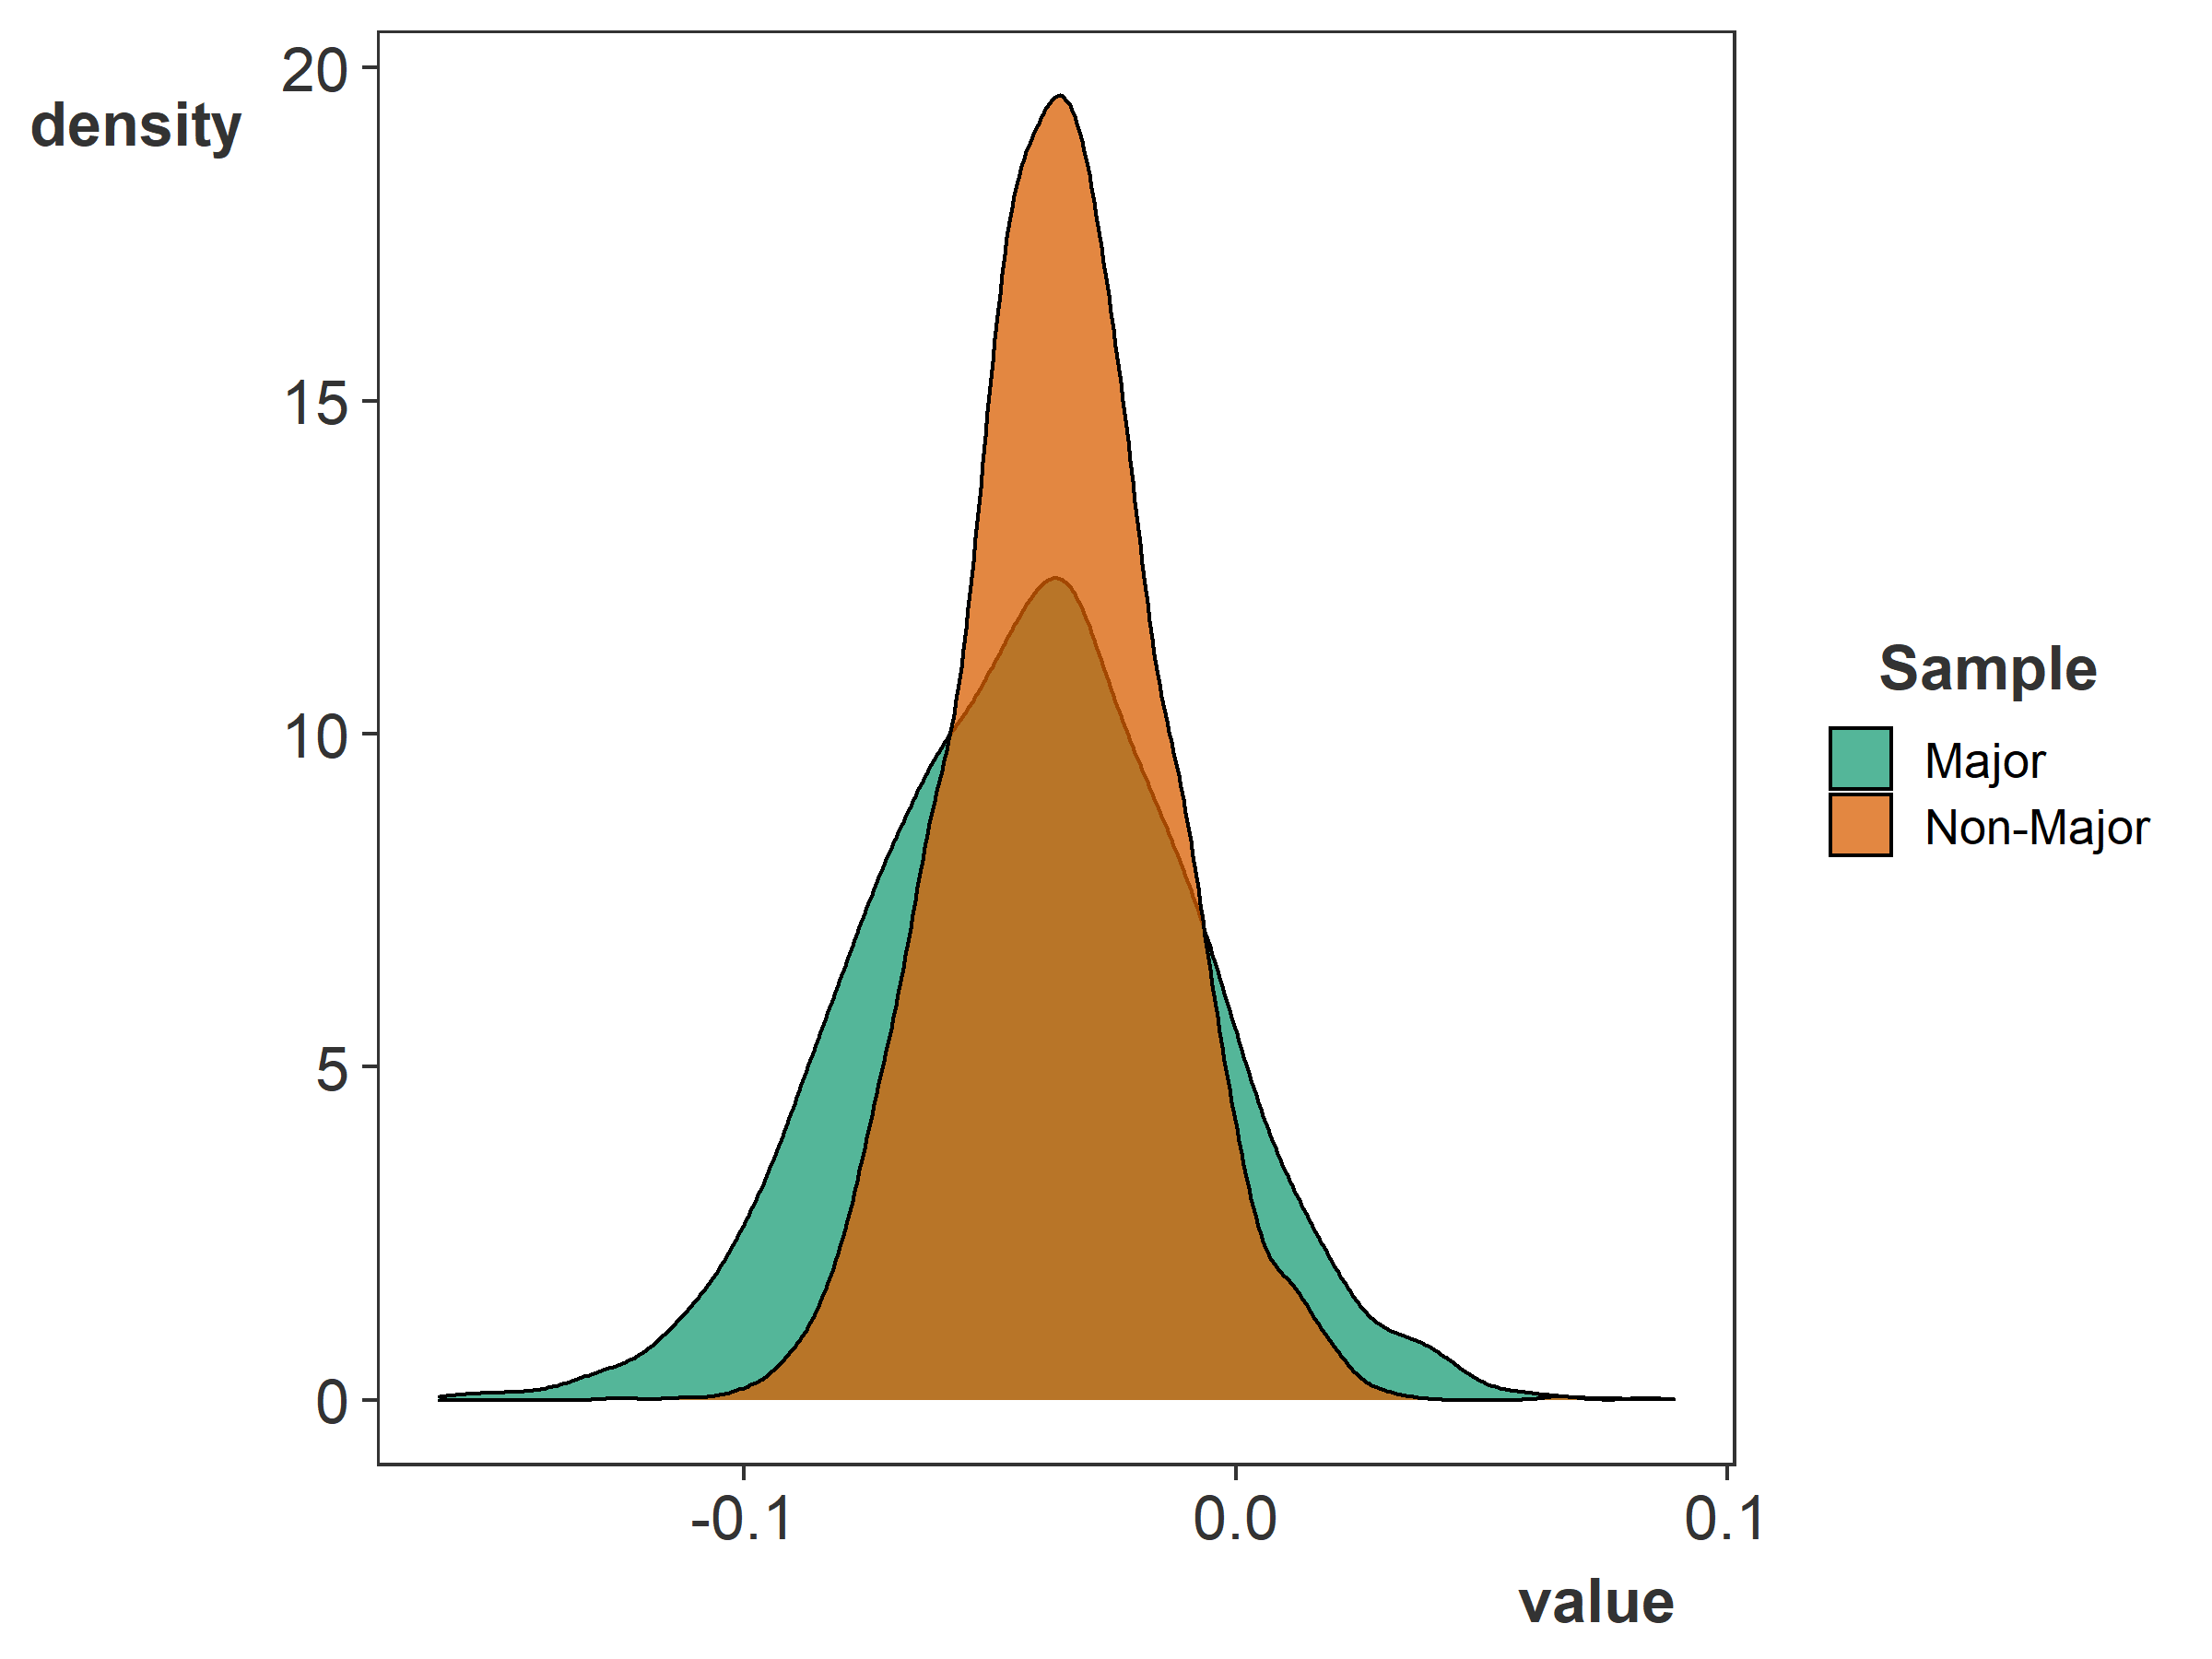
\includegraphics[width=0.95\textwidth]{var-slopes-depth.png}
\end{figure}

\end{frame}

%------------------------------------------------

\begin{frame}{Full Varying Slopes Results}

\begin{figure}[htbp]
	\centering
		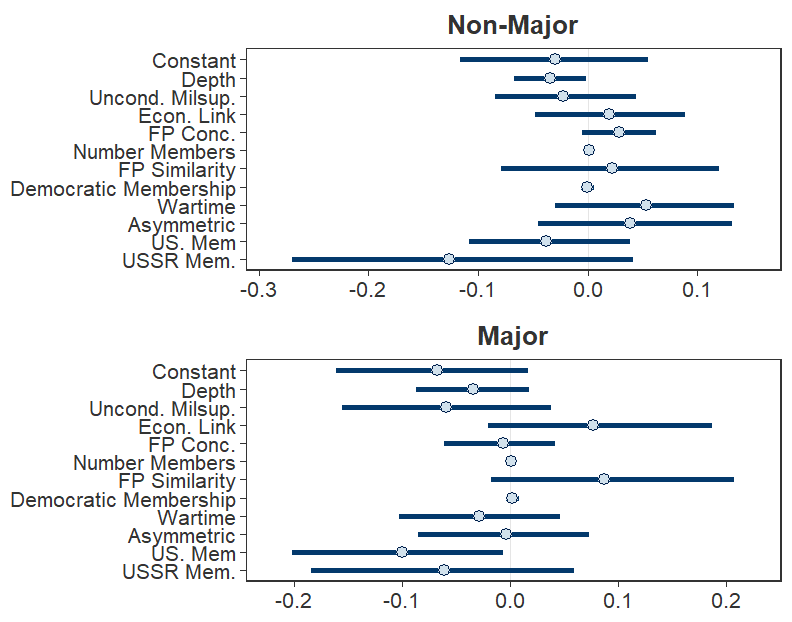
\includegraphics[width=0.95\textwidth]{vs-res-full.png}
\end{figure}

\end{frame}


%------------------------------------------------


\begin{frame}{Single-Level Robust Regression}

\begin{figure}[htbp]
	\centering
		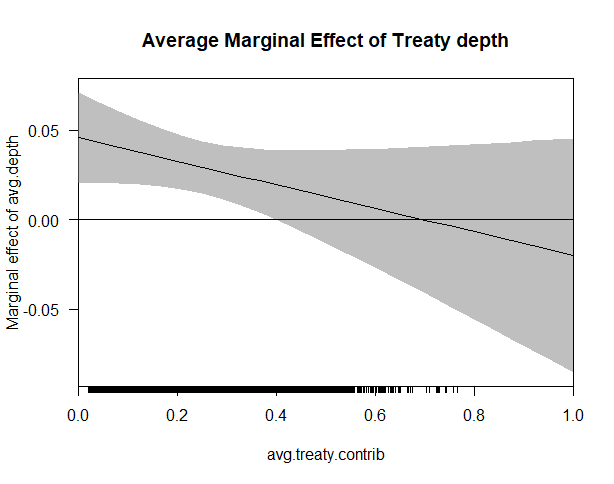
\includegraphics[width=0.95\textwidth]{depth-contrib-margins.png}
\end{figure}



\end{frame}

%------------------------------------------------


\begin{frame}{Binning Estimator Check of Interaction}

\begin{figure}[htbp]
	\centering
		\includegraphics[width=0.95\textwidth]{depth-inter-bin.png}
\end{figure}


\end{frame}


%------------------------------------------------


\begin{frame}{Kernel Estimator Check of Interaction}

\begin{figure}[htbp]
	\centering
		\includegraphics[width=0.95\textwidth]{depth-inter-kernel.png}
\end{figure}


\end{frame}




%----------------------------------------------------------------------------------------

\end{document}